\subsection{Annual variability and daily cycle of clouds}\label{sec:daily_cycle}

Since the cloud classification by hydrometers grouping showed a more comprehensive classification, this algorithm is employed in the following analysis. This section aims to analyze the inter-annual and daily cycle variability of cloud frequency of occurrence at the Granada station. In this framework, a first overview on cloud occurrence is given by the left panel of Figure \ref{fig:cloud_available}, which shows the monthly frequency of occurrence of different sky conditions, categorized into single-layer clouds, multi-layer clouds, clear sky, and noise (as explained in section \ref{sec:new_method}). The data reveal a distinct seasonal pattern in cloud cover and clear sky occurrences. Clear sky conditions (green line) are predominant all year long, being most frequent in the summer months, peaking in July and August (> 80\%), with a significant decline in spring, reaching the lowest point in March and April (40\%). This pattern indicates a higher prevalence of clear skies during the warmer months and increased cloudiness during the colder months. 
Single-layer clouds (blue line) exhibit a relatively weak seasonal pattern throughout the year, with a slight peak in spring (35\%) and a decrease in the summer months (10\%), suggesting a moderate variation in single-layer cloud occurrences. Multi-layer clouds (orange line) show a similar pattern, with a peak in March and April and a reduction during the summer, indicating a seasonal preference for multi-layer clouds in the spring, when there is more multi-layer than single-layer. The noise category (red line) maintains a weak seasonal pattern throughout the year, comparable with multilayer in later spring and summer. 
Overall, the data highlight clear seasonal variations in sky conditions, with clear skies dominating in summer and increased cloudiness, both single and multi-layer, in the cooler months. Since this station exhibits a quite low cloud occurrence, a need to handle multilayer clouds is revealed to fill gaps of cloud properties at regions such as the western Mediterranean. Particularly, these multi-layer are problematic due to inaccurate LWP partitioning, leading to a misclassification of liquid pixels inside clouds, as observed by \cite{tatiananomokonovaStatisticsCloudsTheir2019}. Therefore, the following analyses are focused only on single-layer clouds, seeing their physical properties can be retrieved more accurately.

\begin{figure}[H]
	\centering
	\begin{subfigure}{0.48\textwidth}
		\centering
		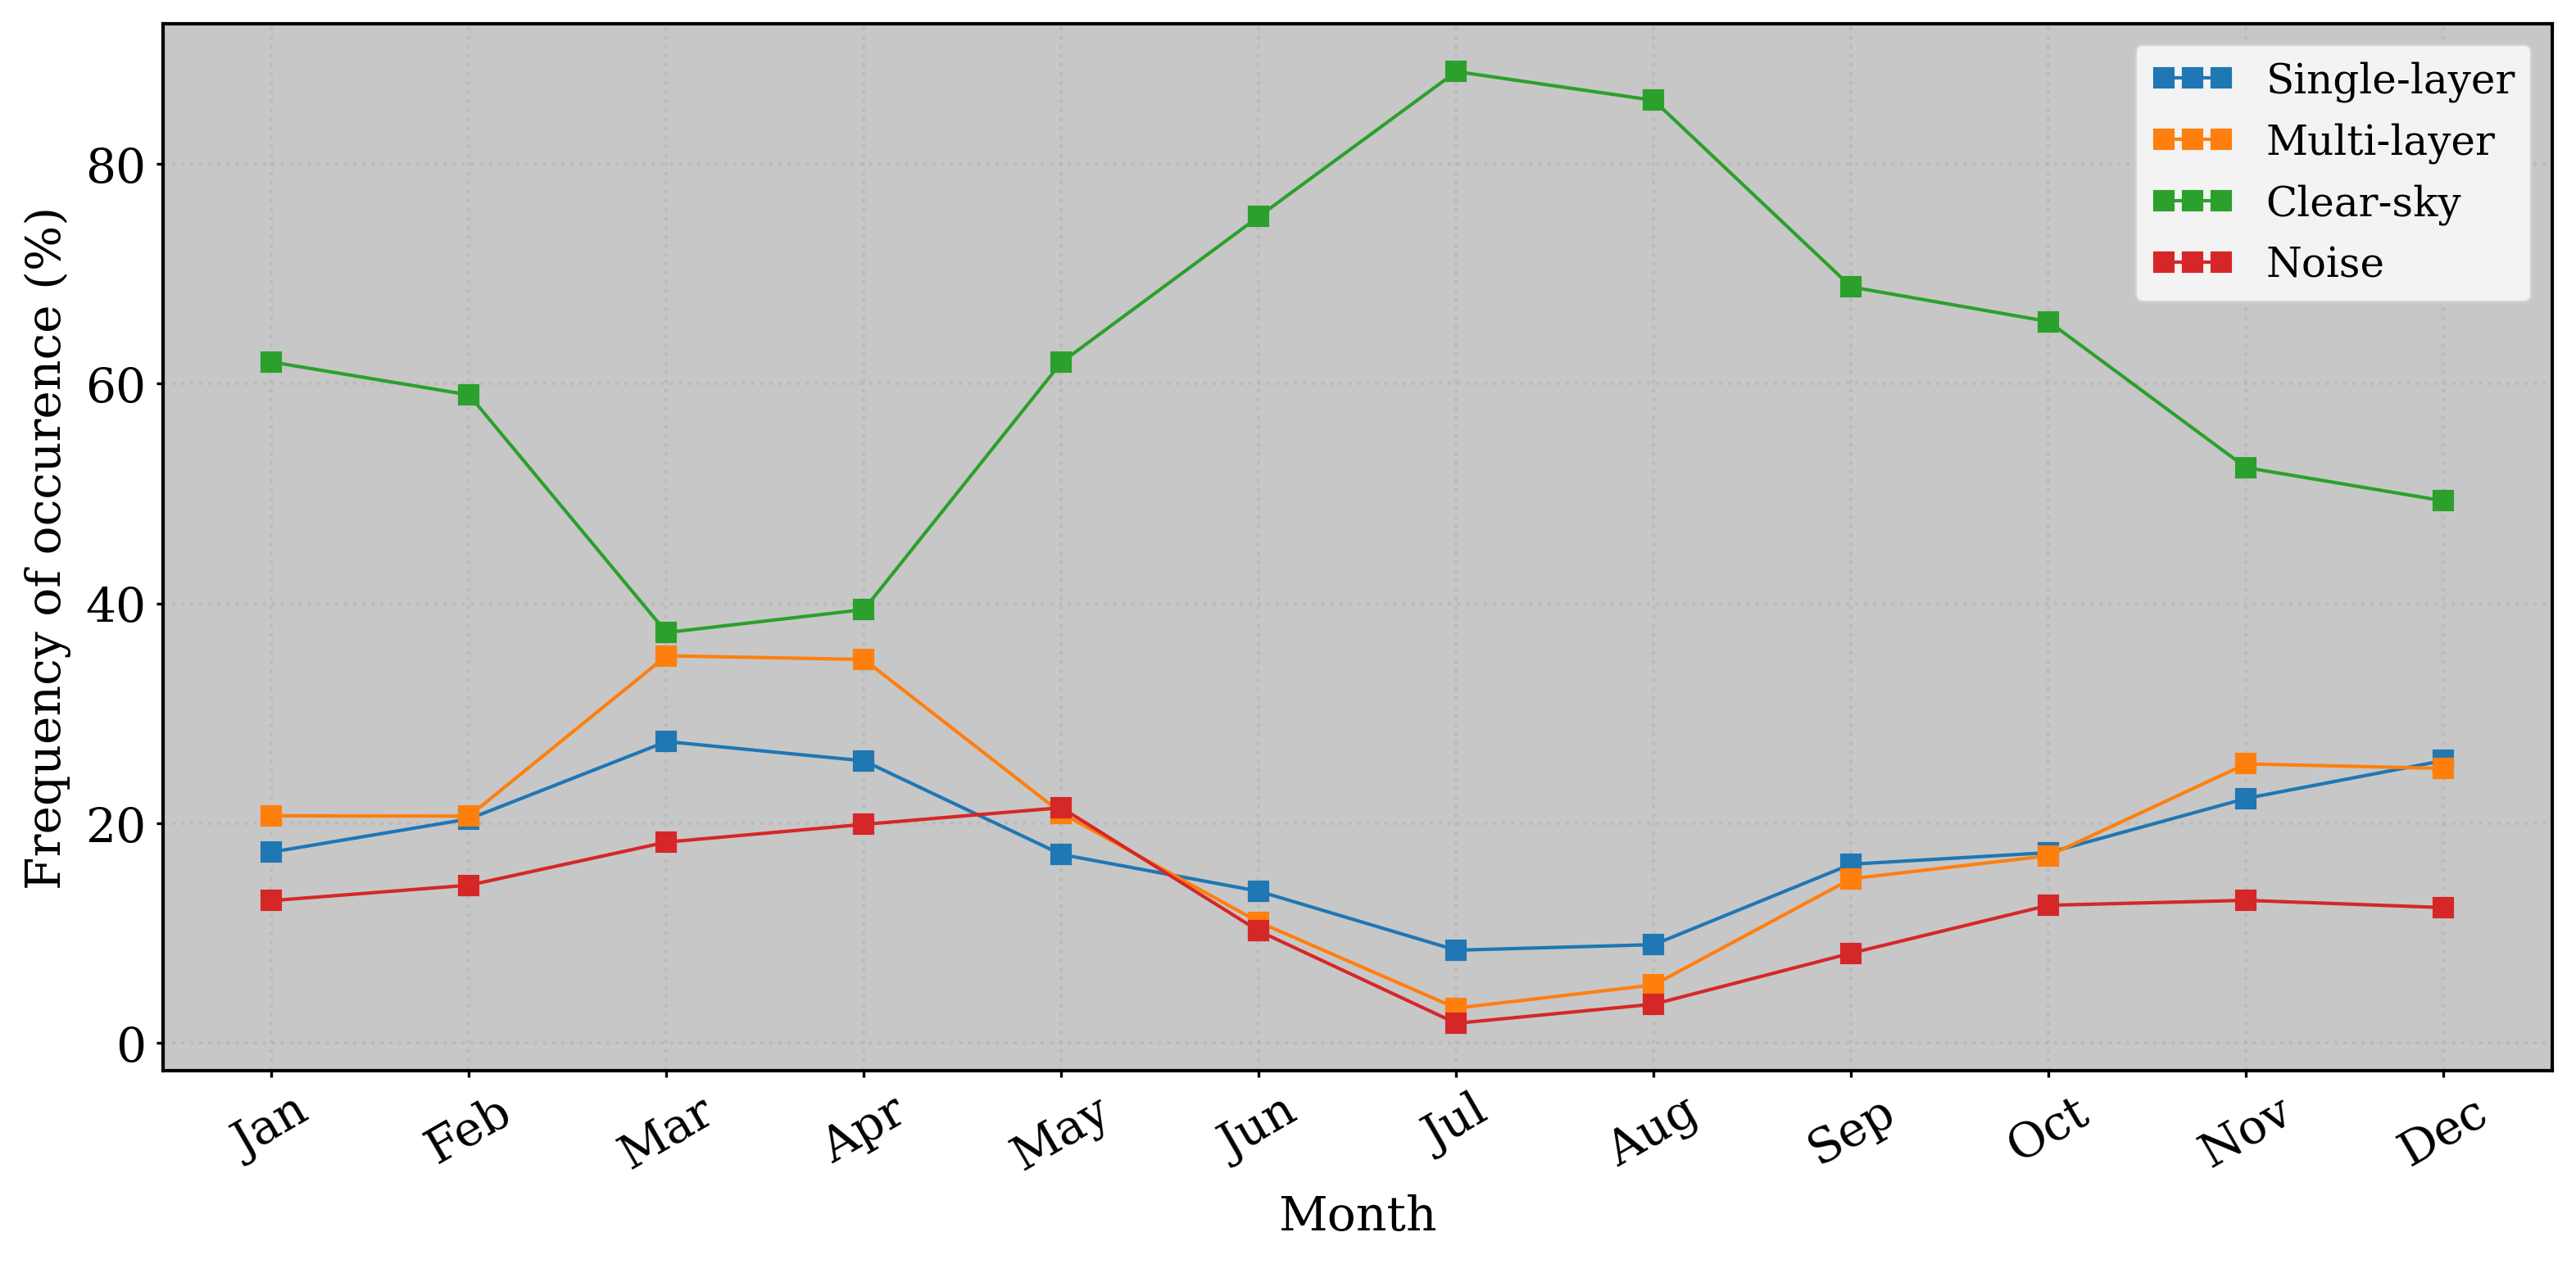
\includegraphics[width=\textwidth]{../../phd_clouds/figures/new_method_monthly_cloud_occurence.png}
		\caption{}
	\end{subfigure}
	\hfill
	\begin{subfigure}{0.48\textwidth}
		\centering
		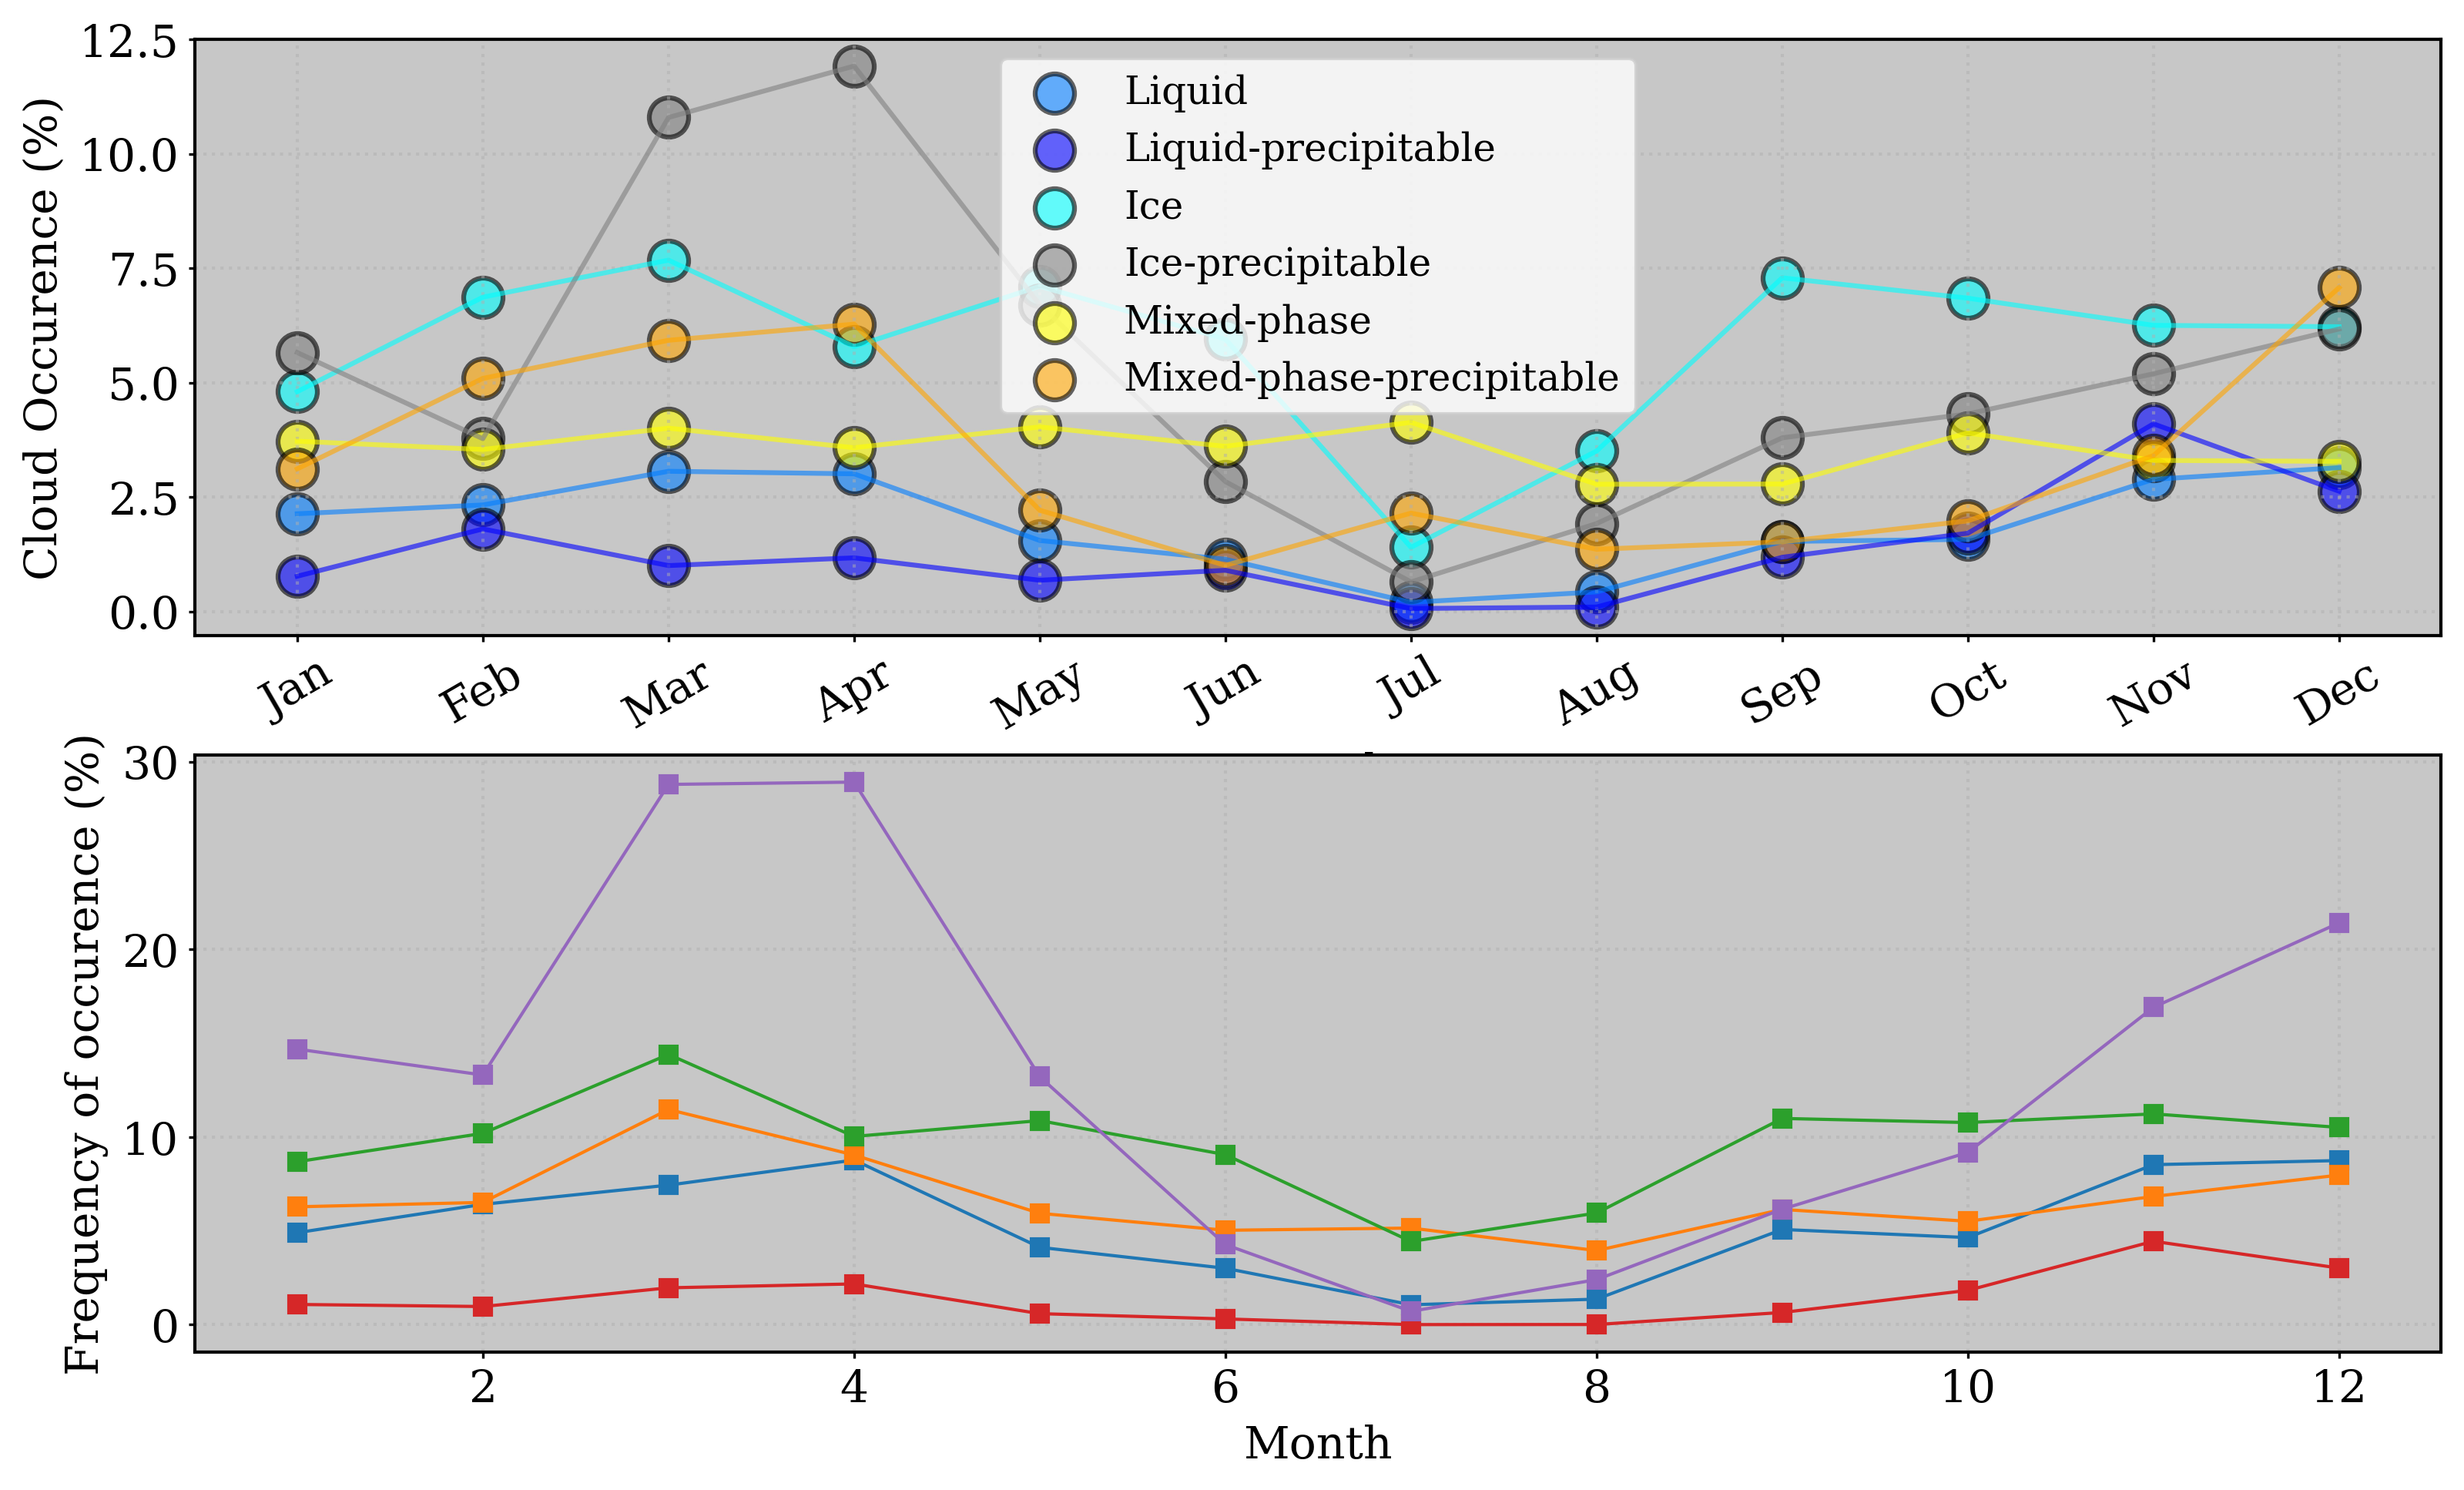
\includegraphics[width=\textwidth]{../../phd_clouds/figures/new_method_monthly_single_layer_frequency}
		\caption{}
	\end{subfigure}
	\caption{On the left, inter-annual frequency of occurrence for single layer clouds (blue), multi-layer clouds (orange), clear sky (green) and noise (red). Right panel, inter-annual single layer cloud occurrence for different cloud categories (see section \ref{sec:new_method}). Each cloud types is indicated in the legend}
	\label{fig:cloud_available}
\end{figure}

Monthly frequency of occurrence is depicted in the right panel of Figure \ref{fig:cloud_available}. Mixed-phase clouds (yellow) exhibit relatively consistent occurrences with slight fluctuations around 3\% and 4\%. Liquid-precipitable (dark blue) has a modest variation with zero occurrence in summer, followed by an increase during the transition to winter, reaching a maximum of 4\% in November, suggesting increased precipitation during fall. Liquid clouds (blue) are more variable, showing a percentage of 3\% in March and December, against zero in summer. Ice clouds (cyan) drop sharply in July and maintain almost constant levels around 5\% and 7\% throughout the rest of the year, indicating hotter temperatures that inhibit ice cloud formation during summer. Ice-precipitable clouds (gray) have a notable peak of 8\% in spring, followed by a decrease in summer (1\%) and an increase in fall, until they reach a local maximum of 5\% during winter. It suggests seasonal variations in ice-related precipitation with maximum in spring, unlike the case of water-related precipitation, which showed a maximum in November. Mixed-phase-precipitable clouds (orange) peak in April (6\%) and December (7\%), indicating higher chances of mixed-phase precipitation towards spring and the end of the year. Overall, ice, precipitating ice, and precipitating mixed-phase clouds have the strongest seasonal pattern, indicating a higher sensibility of ice due to thermodynamic conditions than liquid droplets. Moreover, the precipitation in this region is intrinsically related to ice and mixed phase clouds.

%An important mechanism associated with temperature decreases and responsible for extreme rainfall in Eastern Spain is the occurrence of cut-off lows (COLs). COLs account for nearly all rain events in Valencia, Spain \citep{ferreiraCutOffLowsExtreme2021}, and are likely to affect the Granada station as well. This influence is attributed to the easterly wind component of COLs formed in the warm Mediterranean \citep{porcuStudyCutoffLow2007}, which can reach the station, bringing humidity and cold air masses that favor cloud formation. In Valencia, \cite{ferreiraCutOffLowsExtreme2021} reported the rainiest days occurring in winter, with extreme rainfall events in spring and fall, aligning with our observations. 

During the summer temperatures are higher and just a few non-precipitating clouds were observed at our station. These clouds can be related to convection since we will observe that they have larger thickness and ice water content (IWC) at higher altitudes. Besides elevated temperatures, the Iberian Peninsula experiences a large low-pressure area over northern Africa, with high-pressure systems over the Atlantic Ocean and eastern and central Europe. This results in easterly winds over Andalusia, transporting moisture from the Mediterranean Sea in summer \citep{f.j.bello-millanSimulationsTornadicSupercell2024}. This combination of high temperatures and humidity can create an environment conducive to storm formation in Granada during the summer. In this context, the few clouds observed in summer are likely related to convectively formed cumulus or cumulonimbus clouds. This will be more evident when studying their physical properties in further sections.

Next, the daily cycle of cloud occurrence should uncover the influence of temperature around mid-day, when the solar radiance is more intense. Although we already discuss the influence of synoptic and local phenomena in cloud formation, convection clouds should appear in the diurnal cycle. Figure \ref{fig:cloud_occurence_daily_cycle} displays the diurnal cycle per season, showing no convection for any type of cloud during summer, fall and winter. Despite that fall shows an increase of ice clouds around mid-day, they are probably cirrus clouds, since their median base height and thickness are 8.5\,km and 1.5\,km, respectively (see Figure \ref{fig:cloud_macrophys}).

\begin{figure}[H]
	\centering
	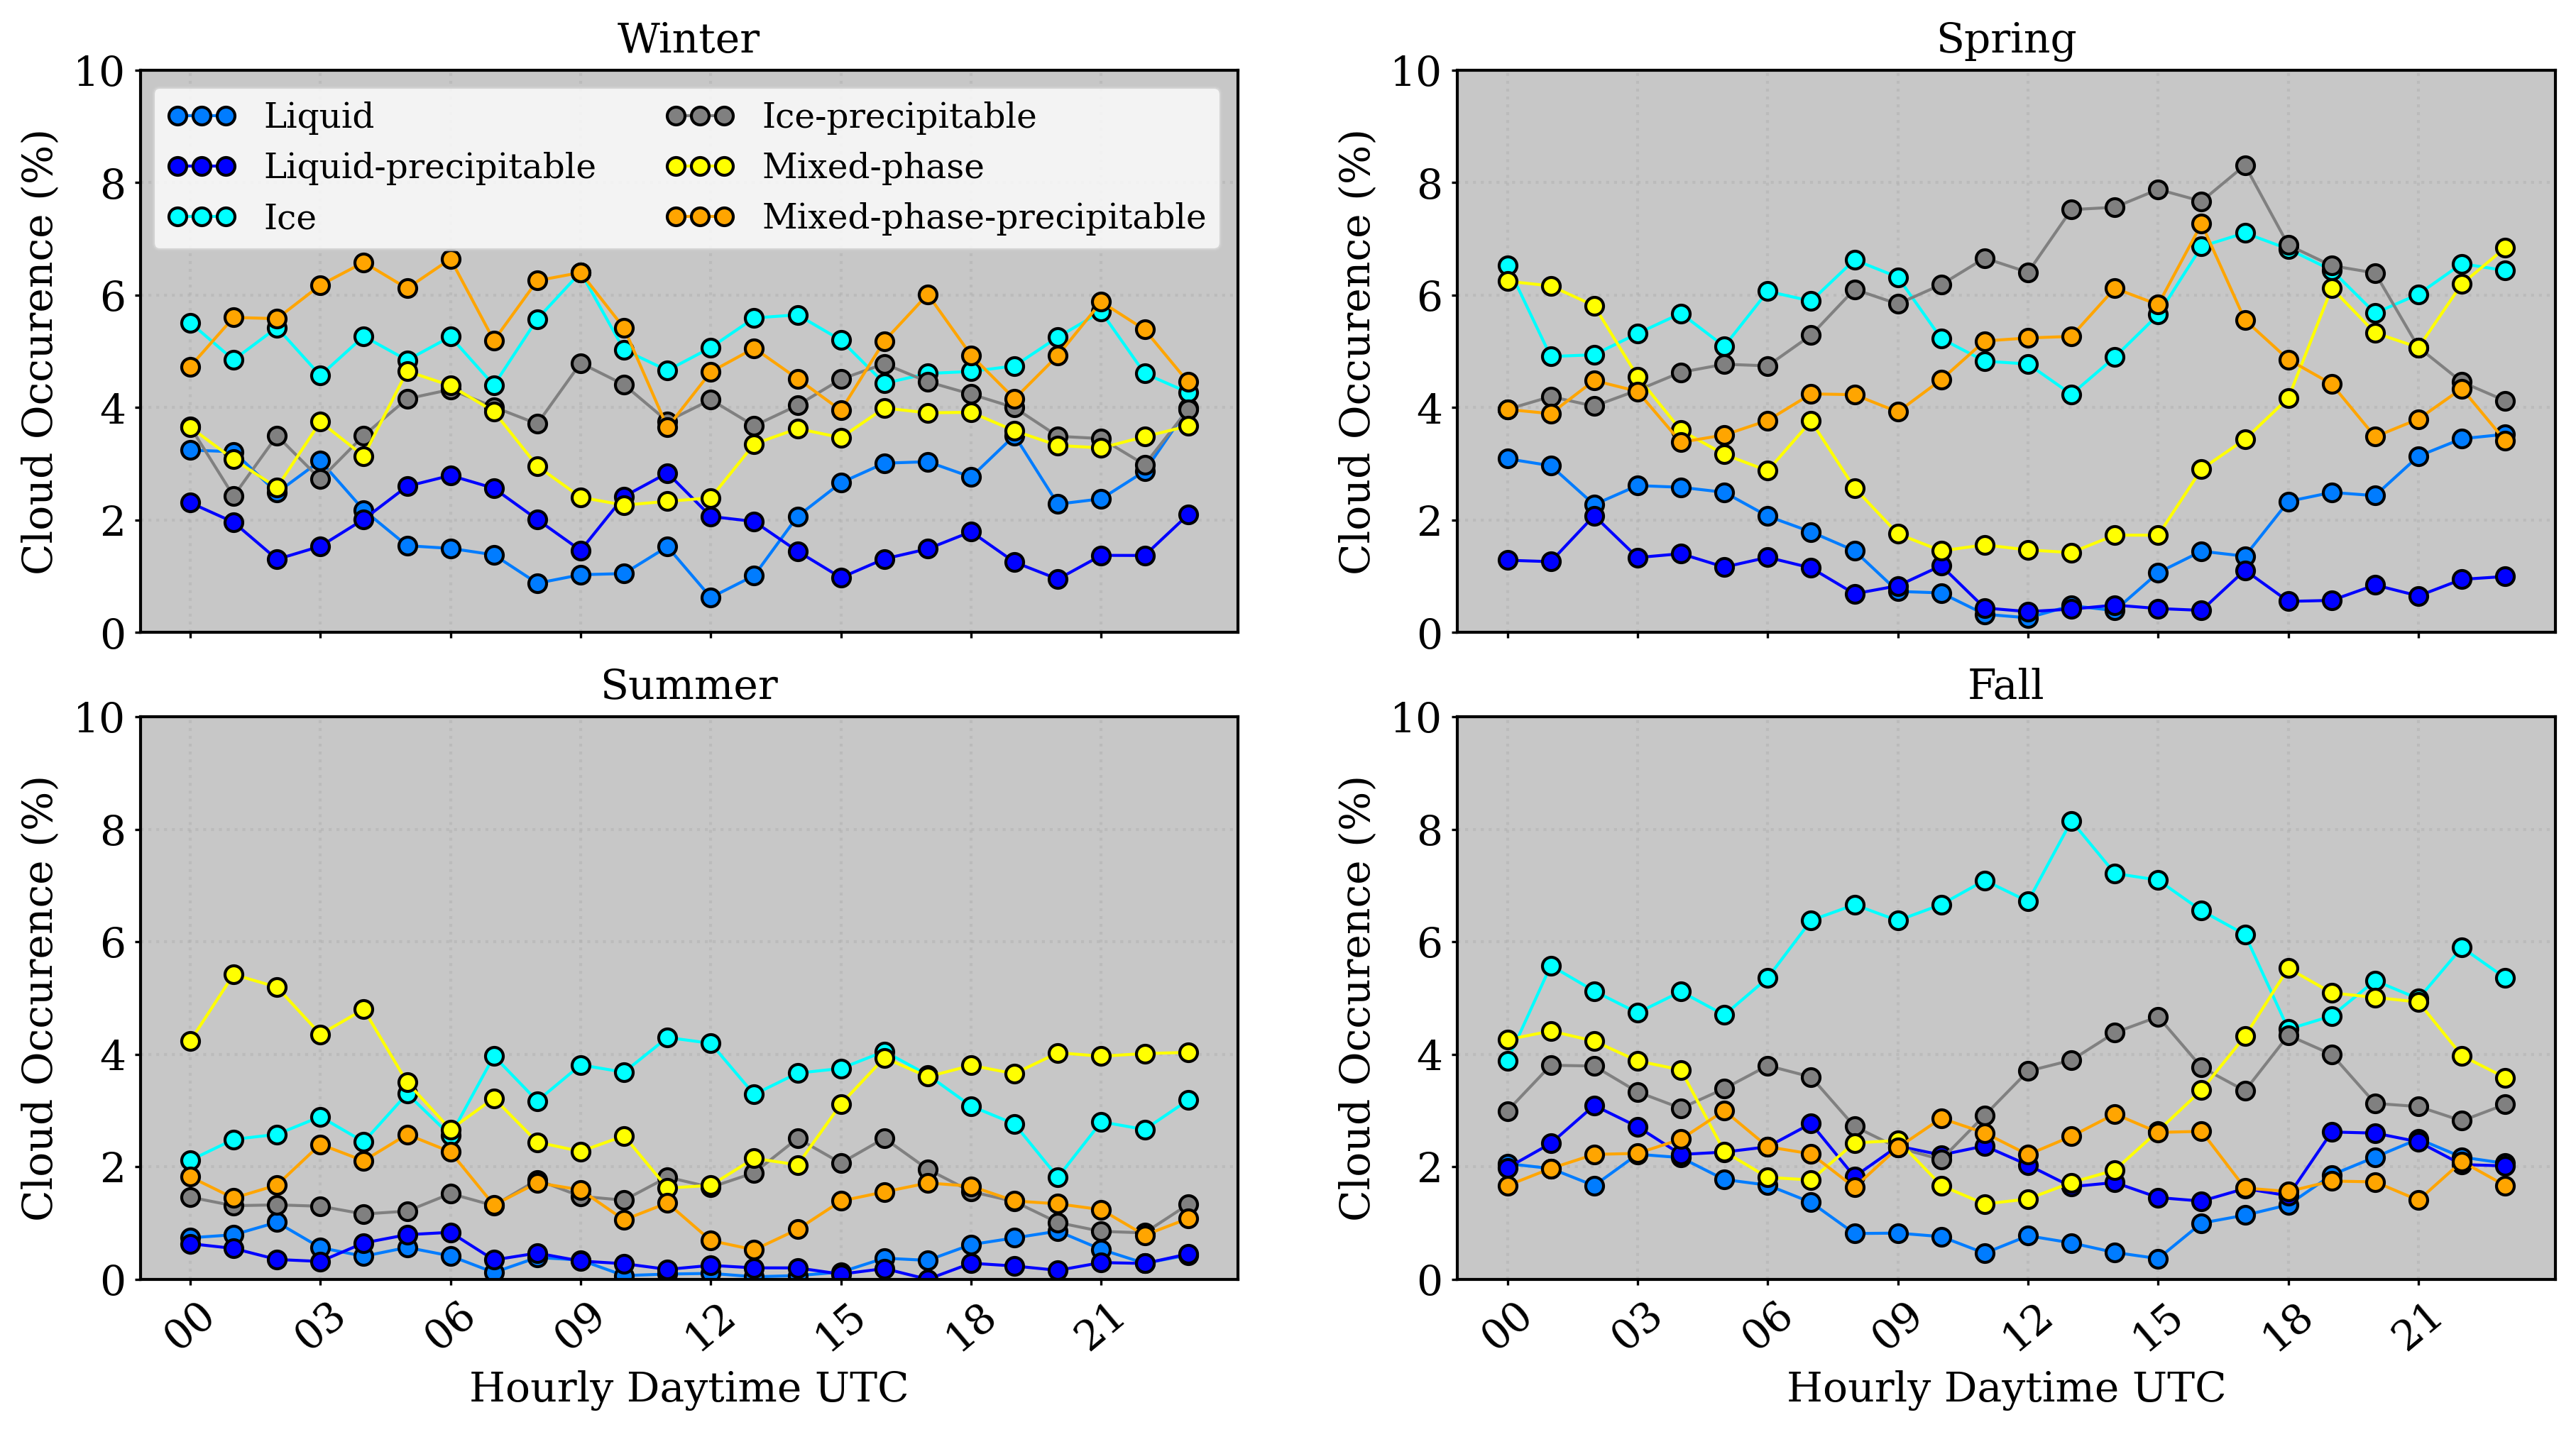
\includegraphics[width=.9\textwidth]{../../phd_clouds/figures/hourly_seasonly_single_layer_frequency}
	\caption{Daily cycle of cloud occurrence per season. The season is indicated in the title of each figure, where winter and spring are in the first row, and summer and fall in the second row. The color of each cloud category is indicated in the legend}
	\label{fig:cloud_occurence_daily_cycle}
\end{figure}

However, spring shows a possible presence of convective clouds, with a slight peak of occurrence for Ice-precipitable and Mixed-phase-precipitable clouds between 09:00 and 21:00 UTC. Different from non-precipitating clouds which reached a minimum around mid-day, these clouds doubled the occurrence from 4\% at 00:00 to 8\% at 16:00-17:00 UTC. These observations are consistent with the findings of \cite{shahiAssessmentSpatiotemporalVariability2022}, where convection-permitting models of the Iberian Peninsula (IP) captured high values of mean precipitation during spring. Additionally, \cite{alexandrerios-entenzaMoistureRecyclingIberian2014} revealed that specific synoptic conditions, such as a reduction in the strength of the zonal circulation, can favor local and mesoscale convection during spring in the western region of the IP. This analysis confirms that the maximum cloud and rain occurrence observed during peak sunlight hours may be strongly associated with local convection. 

\subsection{Seasonal patterns in cloud base, top, and thickness}

Seasonal evolution of cloud base height, top height and thickness are displayed in Figure \ref{fig:cloud_macrophys}. Each color represents a cloud type, where liquid clouds are in blue, ice clouds are in gray and mixed-phase clouds are in orange. Also, the lightest colors represent non precipitating clouds, and the darkest colors represent precipitation clouds. Thus, through cloud base analysis, precipitating clouds exhibit a significantly lower cloud base height (top panel) compared to non-precipitating clouds, as well as a narrower distribution. Regarding non-precipitating ice clouds, they possess the highest cloud base heights, with median values around 8\,km. The ice clouds with base height above the 50/75th percentile can be normally associated with cirrus clouds. Next, non-precipitating mixed-phase clouds have the second highest cloud base, showing considerable variability, except during summer, when values stabilize at 5.5 km. Also, these clouds present a higher base in fall, where the 50th percentile reaches 6.5 km. Differently, the precipitating mixed phase clouds have much less variability and higher cloud base at 4.5 km in summer, as expected. For non precipitating liquid clouds, cloud bases are highly variable during summer, achieving significantly different heights compared with other seasons. Overall, in summer, precipitating mixed-phase clouds, and ice precipitating clouds demonstrate elevated cloud base heights, attributed to the relatively high temperatures and low humidity at this season. Liquid clouds also have elevated base height in summer, however only a few cases were registered, with 50th and 75th percentiles around 4 km and 6 km, respectively. These clouds can be related to stratocumulus and stratus clouds, which were dis-coupled from cumulonimbus at the final stage in summer. 

Following, precipitating clouds also have significantly lower median cloud top height (panels at the center of Figure \ref{fig:cloud_macrophys}) compared to non-precipitating clouds and exhibit a narrower cloud top distribution, except in the case of ice clouds. Non-precipitating ice clouds have median cloud tops around 9-10 km, while ice-precipitable clouds demonstrate highly variable cloud tops. Given their well-defined cloud bases, these clouds exhibit greater cloud thickness, indicative of storm activity at our station.
The cloud tops for liquid clouds mirror the variability of their cloud bases, especially during summer. These clouds exhibit a well-defined cloud thickness, with non precipitating liquid clouds having a thickness around 300 m and precipitating liquid clouds reaching up to 500 m.
Non precipitating mixed-phase cloud tops also present high variability. Nevertheless, they displayed a well-defined cloud thickness, with similar distribution along seasons. Their median cloud thickness is around 400 m, increasing to 500 m for the precipitating case (dark orange), with slightly higher values in summer. In general, non-precipitating mixed-phase clouds have median cloud tops around 7 km during spring, summer, and winter, but reach 8.5 km in fall. Then, precipitating mixed-phase clouds have cloud tops around 3 km in spring, fall, and winter, peaking at 7 km in summer.

\begin{figure}[H]
	\centering
	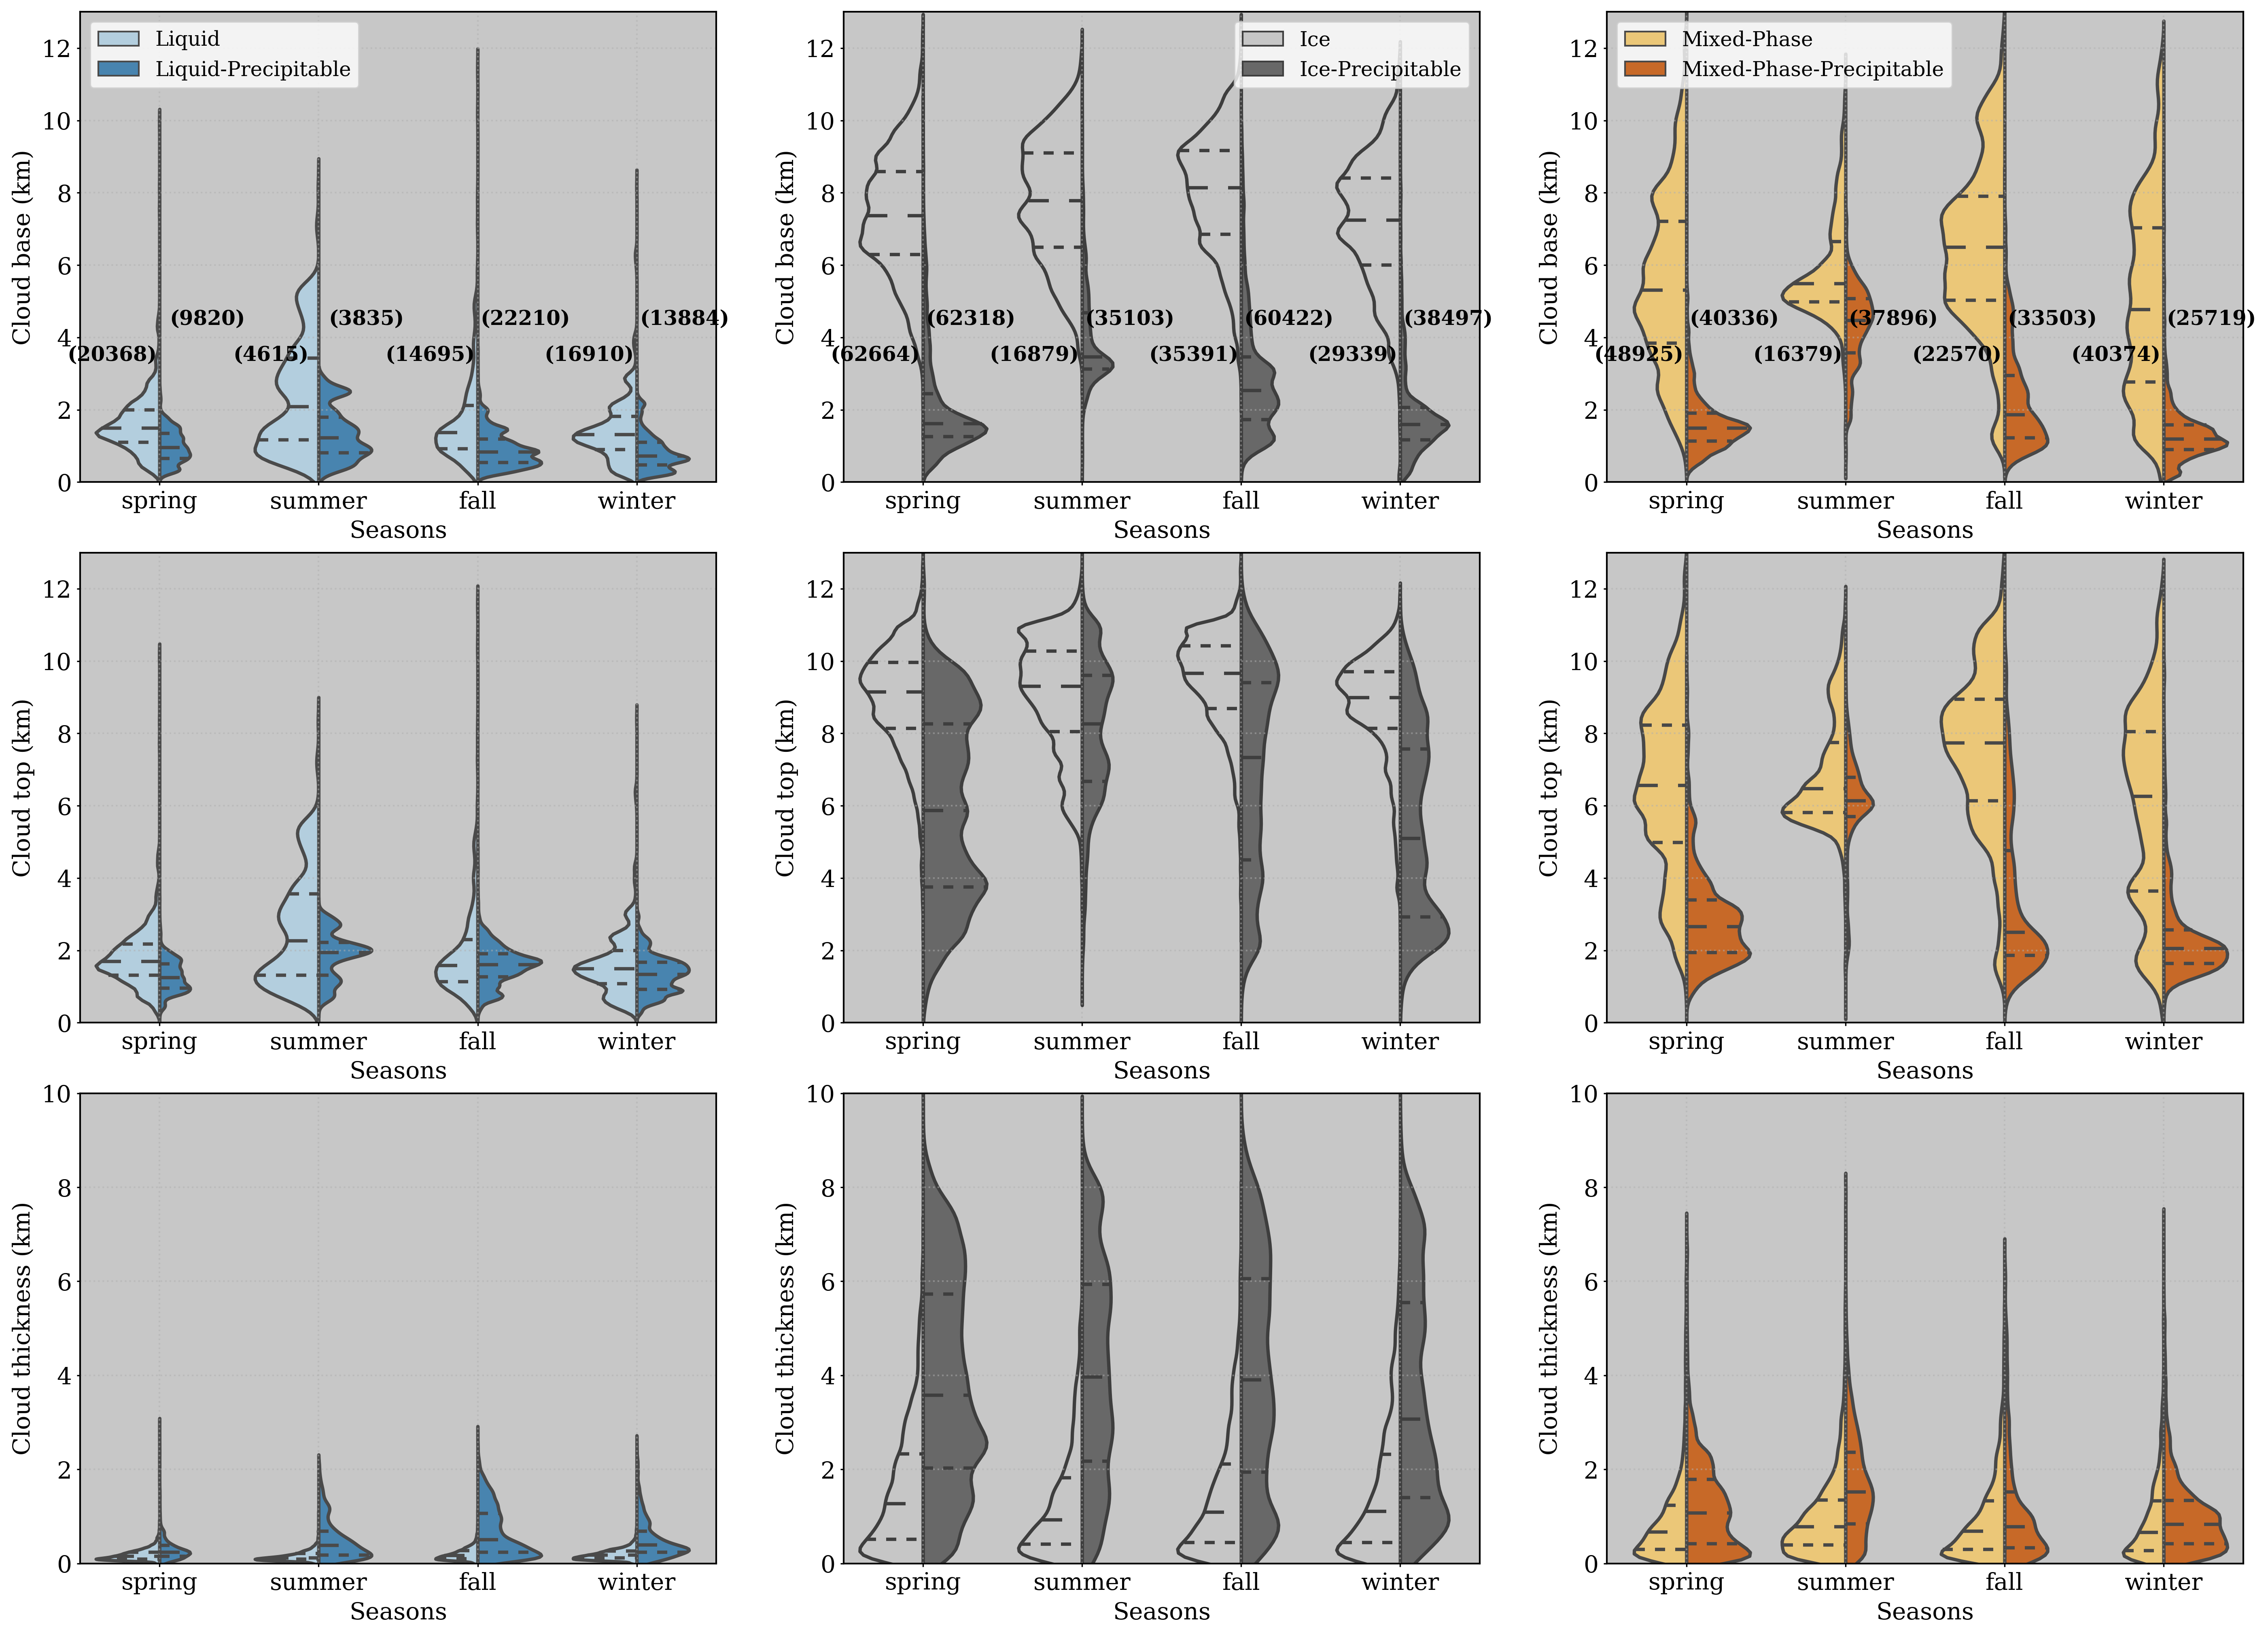
\includegraphics[width=1.\textwidth]{../../phd_clouds/figures/new_method_cloud_prop_violin_season}
	\caption{Seasonal evaluation of cloud base height, top height and thickness. The cloud bases are in the first row, cloud tops in the second row and cloud thickness in the third row. Also, each cloud type is indicated in the legend, where liquid clouds are in the first column, ice clouds in the second column and mixed-phase clouds in the third column. Finally, the dashed lines are indicating the 25/50/75th percentiles}
	\label{fig:cloud_macrophys}
\end{figure}

Overall, ice-precipitable clouds exhibit the greatest cloud thickness, followed by ice, mixed-phase-precipitable, mixed-phase, liquid-precipitable, and liquid clouds. It is important to note that, despite Cloudnet post-processed data being corrected for liquid attenuation, cloud tops for precipitating clouds with higher thickness can be underestimated due to high liquid attenuation.

\subsection{Cloud microphysics properties}\label{sec:cloud_microphys}

\subsubsection{Liquid clouds}

The monthly median profiles of LWC shows high variability of LWC in function of height for liquid clouds (Figure \ref{fig:LWC_liq}, right panel, marked by hot colors and constant lines of 1000 mg m$^{-3}$). For particular months such as February, March and April, a notably variability below 1 km and within 2.5 and 4 km (right panel of Figure \ref{fig:LWC_liq}) is observed. Nevertheless, above 500 m, really high values observed in the monthly profiles are not representative of the entire season as can be seen in the left panel of Figure \ref{fig:LWC_liq}. This figure shows no clear pattern with altitude at any season, LWC is generally presenting a random fluctuation around to 50 mg m$^{-3}$. Differently, below 500\,m, a sharp peak of about 500 mg m$^{-3}$ can be clearly identified in spring. This peak is related to liquid clouds during the springs of 2020, 2021 and 2022 (not shown), at this period. Except for the near surface largest LWC observed in spring, no clear differences were observed between seasonal profiles. Following, summer exhibited a lack of liquid phase clouds, with some elevated LWC at higher levels as shown in the left panel of Figure \ref{fig:LWC_liq}.

Next, the average liquid water path (LWP) (bottom panel of Figure \ref{fig:LWC_liq}, black star) shows a considerable variability of LWP from January to June (also early fall). It highlights a very wide variety of liquid clouds in these months. Also, a notable increase in the median LWP occurs in April, aligning with their maximum cloud occurrence. From August to October, there is a gradual increase in average LWP (marked by the black star), while the median stays stable. This trend corresponds with the increased occurrence of liquid clouds from summer to fall, impacted by different mechanisms of cloud formation. Since these months reported just a few occurrences of liquid clouds, as can be checked by the blue line, which shows the number of cloud profiles per month, their statistics will be much more sensible to these mechanisms. As a result LWP in summer is the smallest, and there is no significant difference between the average and the median.

\begin{figure}[H]
	\centering
	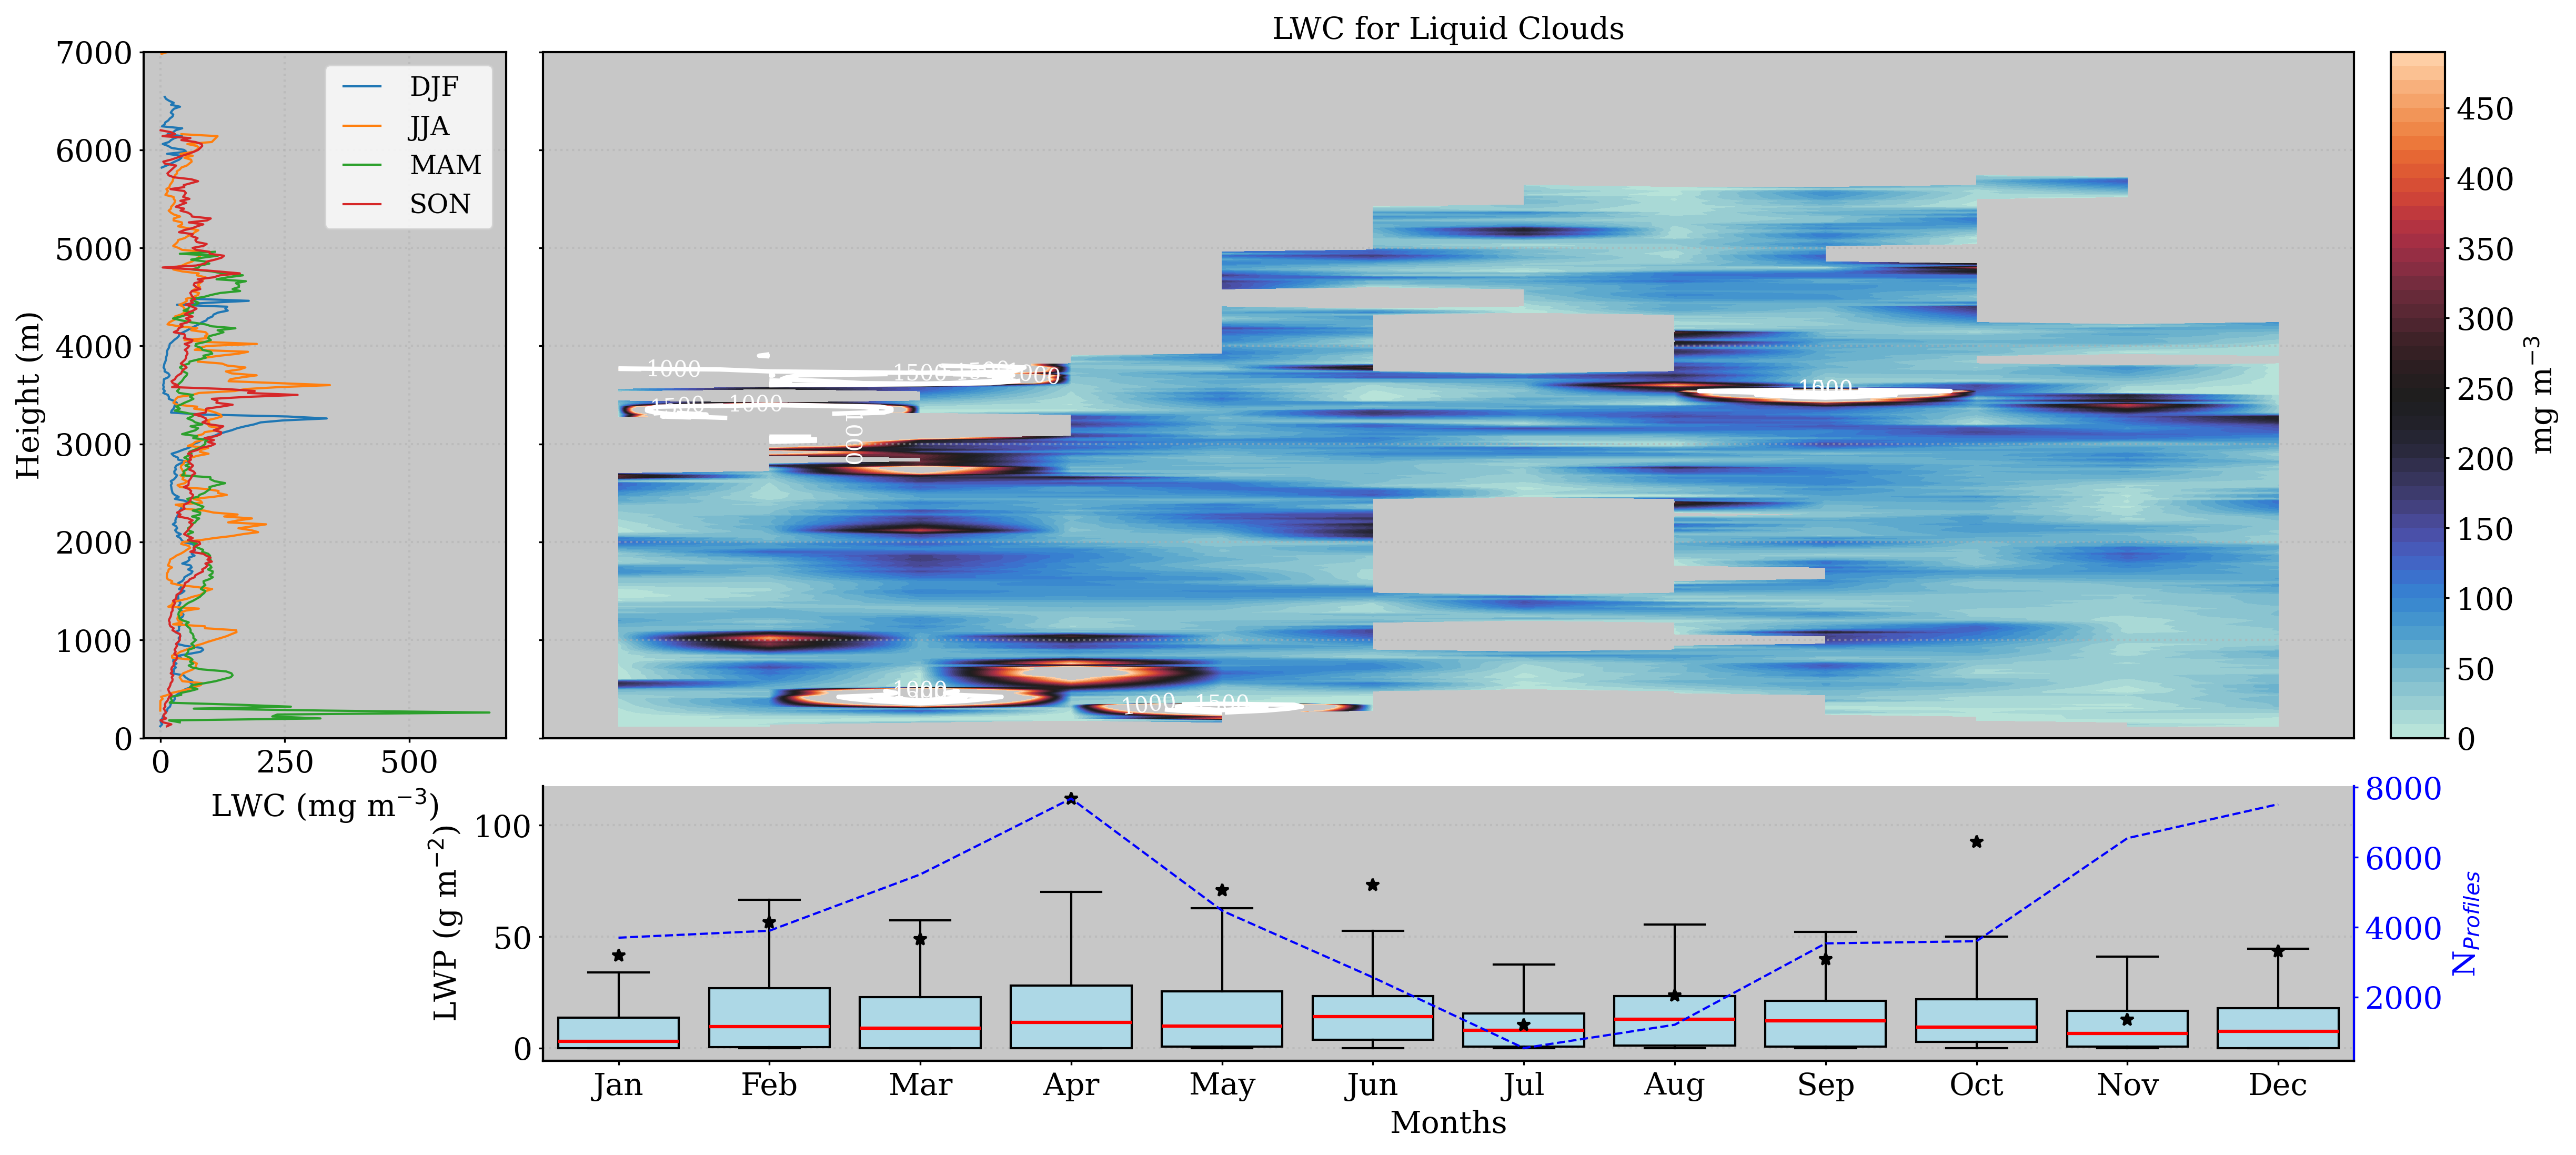
\includegraphics[width=.9\textwidth]{../../phd_clouds/figures/grouped_by_month_evolution_for_lwc_Liquid_mesh}
	\caption{Seasonal and monthly average of liquid water content (LWC) and liquid water path (LWP) for liquid clouds. Left panel shows the seasonal median profiles of LWC. 
		%      where the shaded area indicates the standard deviation divided by 10. 
		Right panel shows the monthly median profiles of LWC and monthly box-plot of LWP in the bottom. For the boxplots, medians are denoted by red lines and the average by black stars.} 
	\label{fig:LWC_liq}
\end{figure}

In terms of droplet effective radius, liquid clouds are well consistent throughout the year, showing small differences in terms of median values (top panel of Figure \ref{fig:DER_liq}), mostly ranging between 5 and 9 $\mu$m. There is no discernible pattern in $r_{liq}$ across seasons, with higher altitudes weakly correlating to larger droplet sizes. In addition, there are almost no liquid droplets above 4 km, just a few occurrences in summer and early fall were registered.

However, the $r_{liq}$ is generally stable around 5 $\mu$m, with a small decrease in July, when almost no clouds were registered. The seasonal profiles confirm the uniformity in $r_{liq}$ distribution with height, showing minimal variation with altitude. It suggests a consistent cloud composition and droplet size throughout different atmospheric conditions. These findings underscore the stable nature of liquid clouds in terms of droplet size and LWC. Normally, these clouds have a small thickness, do not presenting a wide range of $r_{liq}$

\begin{figure}[H]
	\centering
	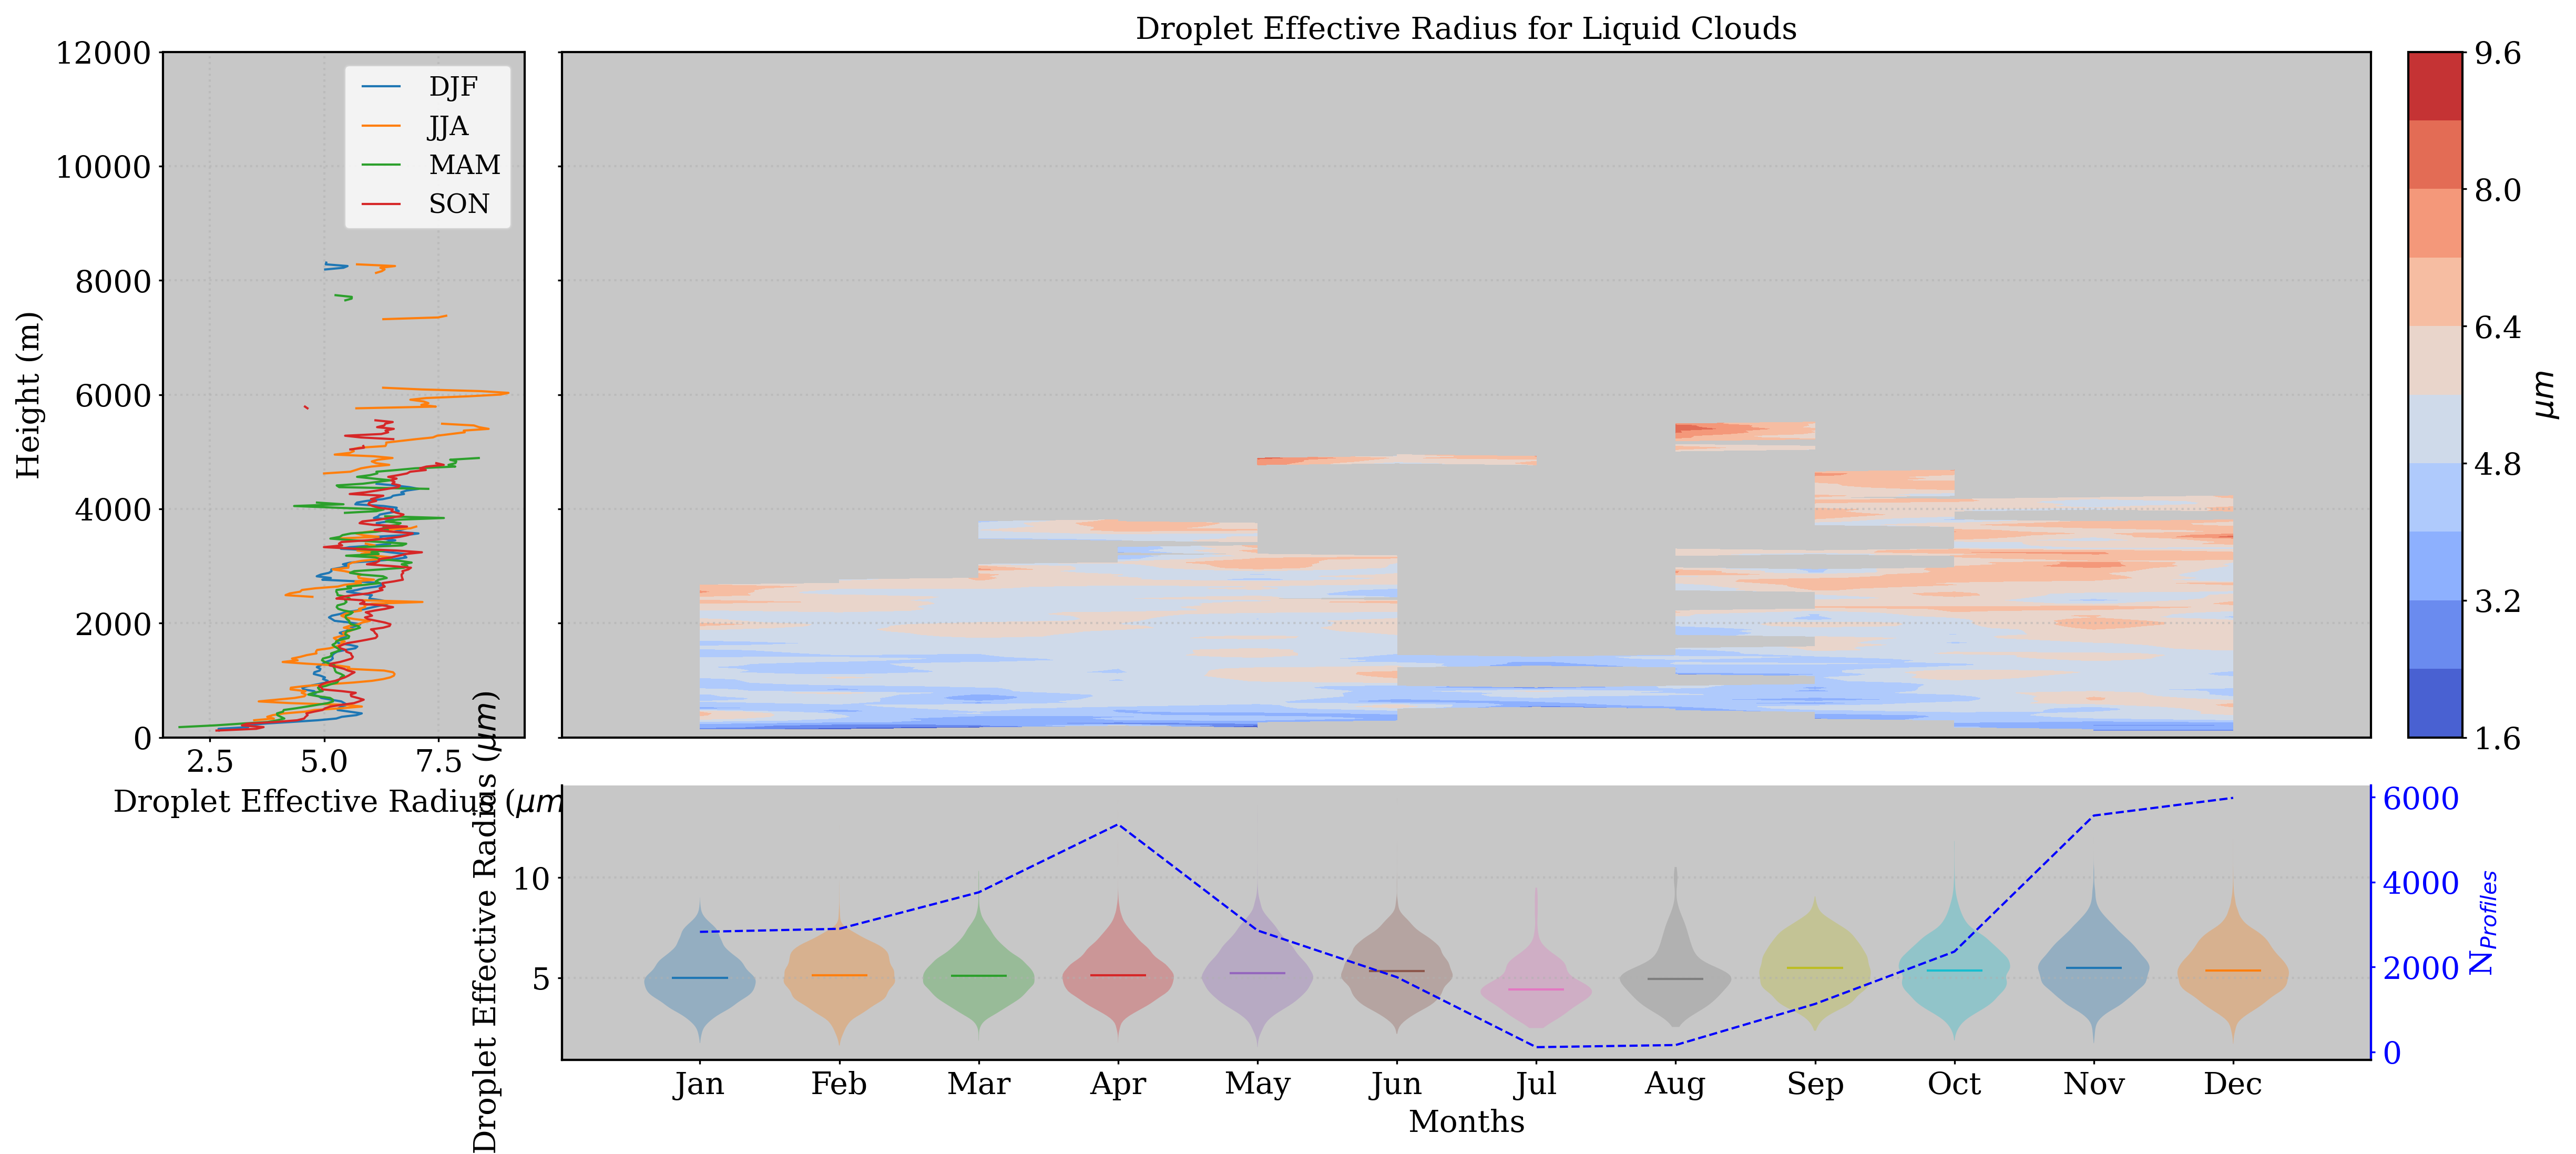
\includegraphics[width=.9\textwidth]{../../phd_clouds/figures/grouped_by_month_evolution_for_der_Liquid}
	\caption{Seasonal and monthly statistics on droplet effective radius ($r_{liq}$) distribution for liquid clouds. Left panel shows the seasonal median profiles of droplet effective radius. Top-right panel shows the monthly profiles of the median $r_{liq}$, while the bottom-panel displays the size distribution of $r_{liq}$ by months.}
	\label{fig:DER_liq}
\end{figure}

For precipitating liquid clouds, significant liquid water content (LWC) is primarily found below 3 km (top-right panel of Figure \ref{fig:LWC_pre_liq}), consistent with their median top heights. Next, regions with significant values of liquid water content show broader areas, which is expected as these clouds are thicker than purely liquid clouds. Monthly median profiles indicate that higher amounts of liquid water content occurs in later fall, winter and spring. However, the highest amount of LWC is identified in June (early summer), very close to the ground (300 m), which is related to only a few cases of these clouds registered in summer (see the blue line in the bottom panel). Then, in the rest of summer and early fall, atmospheric water content is almost zero. In spring, significant values are found even closer to the surface, explained by relatively humidity months in 2020, 2021, and 2022 as already observed for non precipitating liquid clouds. At the last, winter shows a peak of LWC of about 
250 mg m$^{-2}$ at 2 km. 

Overall, the seasonal profiles of LWC emphasizes a clear increase of LWC in function of height during fall, winter and summer. For the last, two peaks of 250 mg m$^{-3}$ are clearly identified at 2 and 3 km, respectively. This season presented more variability with height, showing more peaks of LWC in function of height. Next, fall and winter also presented a peak of about 250 mg m$^{-3}$ at 2 and  2.5 km, respectively. In terms of LWP, Figure \ref{fig:LWC_pre_liq} below indicates substantial variability of LWP in January, suggesting a diverse variety of liquid clouds during this month. In contrast, spring exhibits relatively consistent LWP across its months, reflecting a stable period for precipitating liquid clouds. In these months, their median stays below 50 g m$^{-2}$, and summer has even less LWP, except for June, as previously observed.

\begin{figure}[H]
	\centering
	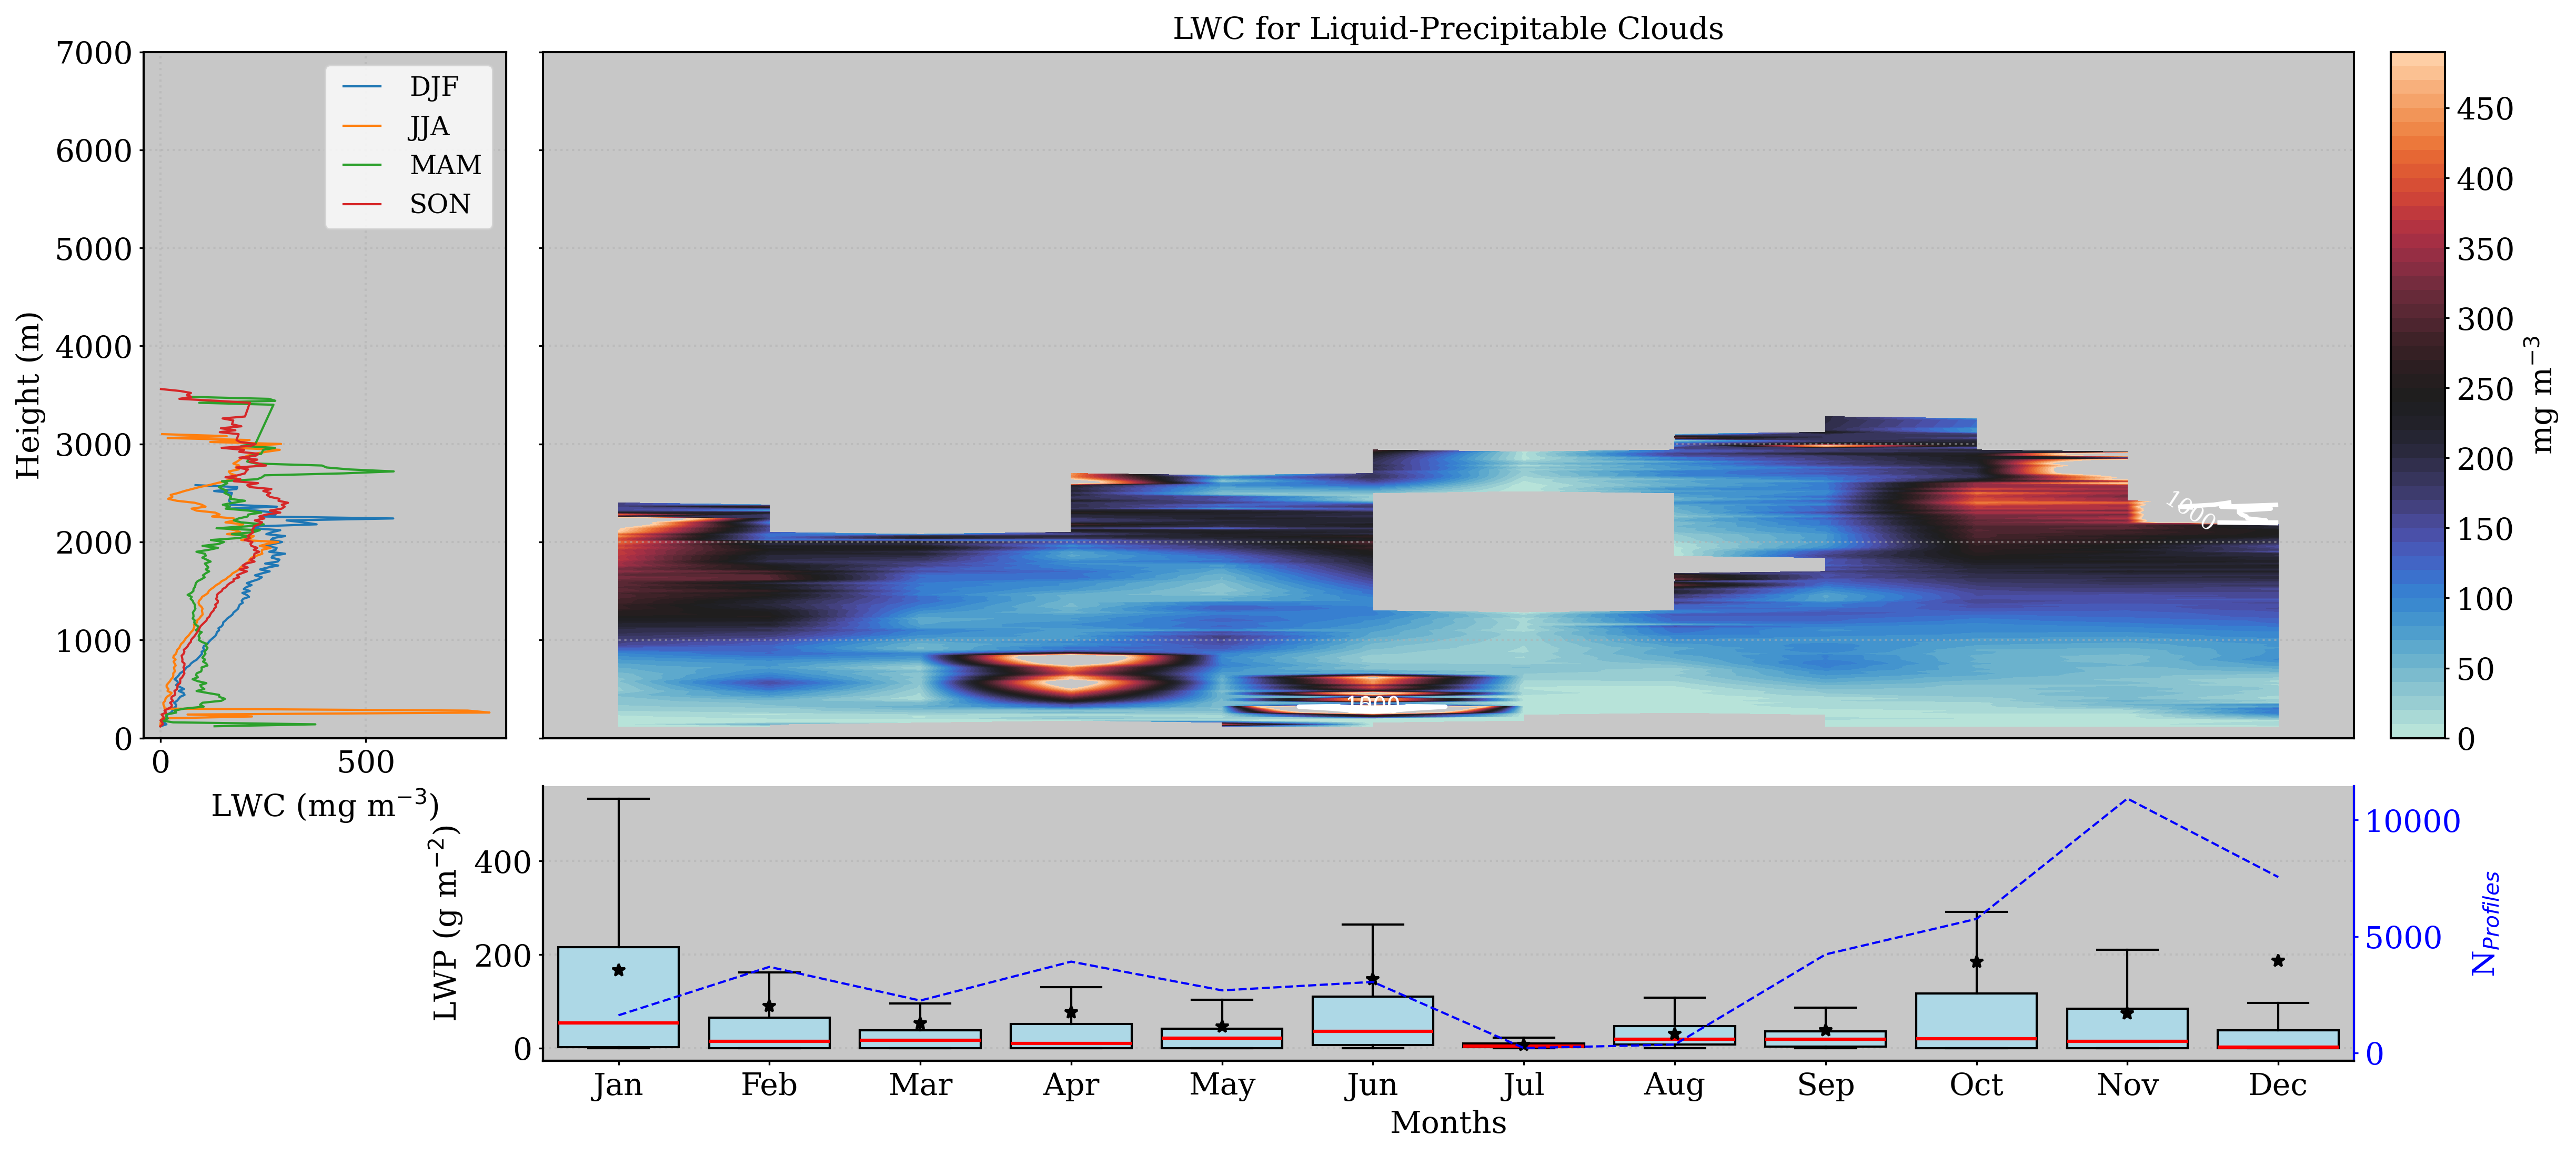
\includegraphics[width=.9\textwidth]{../../phd_clouds/figures/grouped_by_month_evolution_for_lwc_Liquid-Precipitable_mesh}
	\caption{Same as Figure \ref{fig:LWC_liq}, but for precipitating liquid clouds.}
	\label{fig:LWC_pre_liq}
\end{figure}


Different for the purely liquid clouds, precipitating liquid clouds demonstrated radically different seasonal profiles of median $ r_{liq} $ (see Figure \ref{fig:DER_pre_liq}). In spring and summer, the $ r_{liq} $ is smaller than fall and winter the closer to the ground, as can be seen by light blue and warm colors. In addition, $ r_{liq} $ in fall are the largest, often around 15 $\mu$m below 2 km. These sizes are normally related to drizzle droplets, which are more present in this season. The highest median $ r_{liq} $ on the ground in the left panel of Figure \ref{fig:DER_pre_liq} is also related to drizzle particles. This panel also shows that summer and winter exhibit similar $ r_{liq} $ values up to 2 km of altitude, around 10 $\mu$m, decreasing to approximately 5 $\mu$m at 4 km. On the other hand, spring shows an increase of $ r_{liq} $ from 5 $\mu$m to a peak of 15 $\mu$m around 3 km altitude. 

Their monthly size distribution in the bottom panel displays different size distributions over the year, where higher median values are found in fall as already observed, specially in November. During spring and early summer, the median is maintained around 10 $\mu$m, then decreases in summer, and increases again in fall as expected.

\begin{figure}[H]
	\centering
	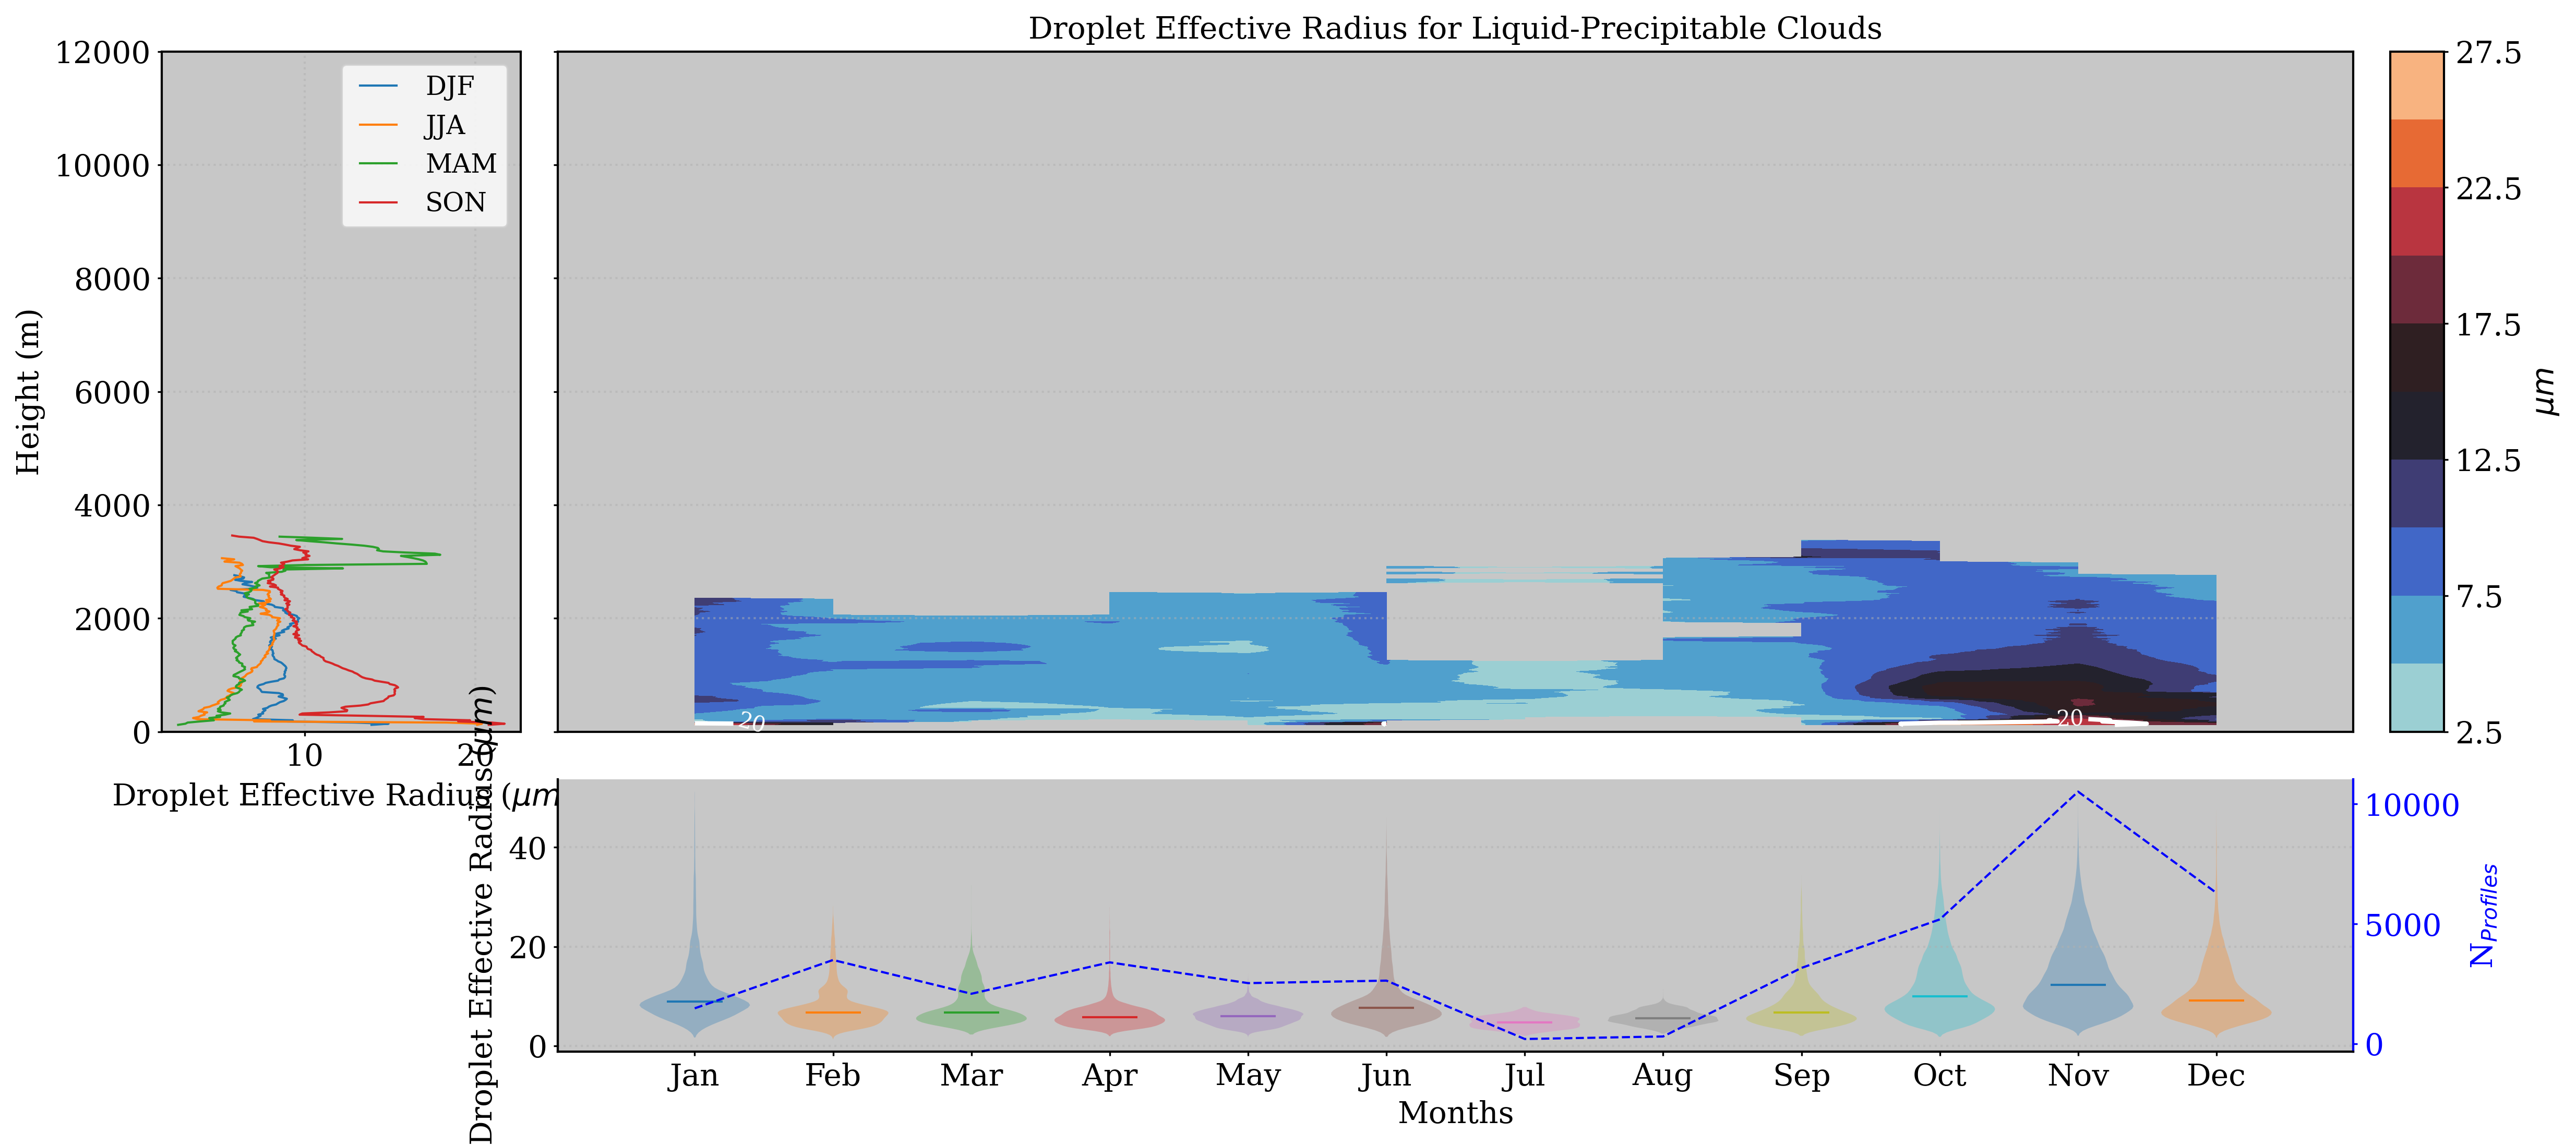
\includegraphics[width=.9\textwidth]{../../phd_clouds/figures/grouped_by_month_evolution_for_der_Liquid-Precipitable_mesh}
	\caption{Same as figure \ref{fig:DER_liq}, but for precipitating liquid clouds.}
	\label{fig:DER_pre_liq}
\end{figure}

Liquid clouds are challenging to analyze due to their low frequency of occurrence. They exhibit significant variability with height, making it difficult to discern seasonal differences in liquid water content (LWC) profiles, except at low levels. Near the surface, LWC is much higher in spring, though their droplet size ($r_{liq}$) remains relatively constant around 5 $\mu$m. In contrast, precipitating liquid clouds display a more pronounced seasonal pattern, with higher LWC and larger $r_{liq}$. Notably, the presence of drizzle particles near the surface is associated with larger $r_{liq}$. During summer, these clouds exhibit two distinct peaks in LWC in function of height, one at 2 km and another at 3 km

\subsubsection{Mixed Phase clouds}

Next, mixed-phase clouds indicate generally lower liquid water content (LWC) values compared to liquid-phase clouds (top-right panel of Figure \ref{fig:LWC_mixed}). These clouds have a consistent occurrence throughout the year (around 3-4\%), but exhibit very high variability of LWC in function of height, as expected since their cloud base also has such variability. Especially in summer and winter, high LWC are encountered above 8 km, surpassing 1000 mg m$^{-3}$. As for the liquid cloud case, these values occur just a few times at this level, and do not affect the seasonal median (left panel of Figure \ref{fig:LWC_mixed}), since other summer-months have much smaller LWC at this height.

Although LWC varies greatly during winter, spring and fall, with most pronounced occurrences below 4 km, their integral remains really close to zero over the year. This can be observed by the bottom panel of Figure \ref{fig:LWC_mixed}, which shows an absence of LWP throughout the entire year in terms of the median. On the other hand, just a few cases with elevated values are generating high mean LWP, highlighting the presence of outliers. Next, vertical profiles of median LWC by season denoted high variability below 4 km and above 10 km, for all stations. Between this level, LWC is relatively small at all seasons, fluctuating around zero. Otherwise, median LWC have local maximums around 100 mg m$^{-3}$, with two notable peaks surpassing 500 mg m$^{-3}$ at 500 m during spring and summer (same case as for liquid clouds). These seasonal variations underscore the complex and dynamic nature of mixed-phase cloud formation and their differing behaviors across various atmospheric conditions.

\begin{figure}[H]
	\centering
	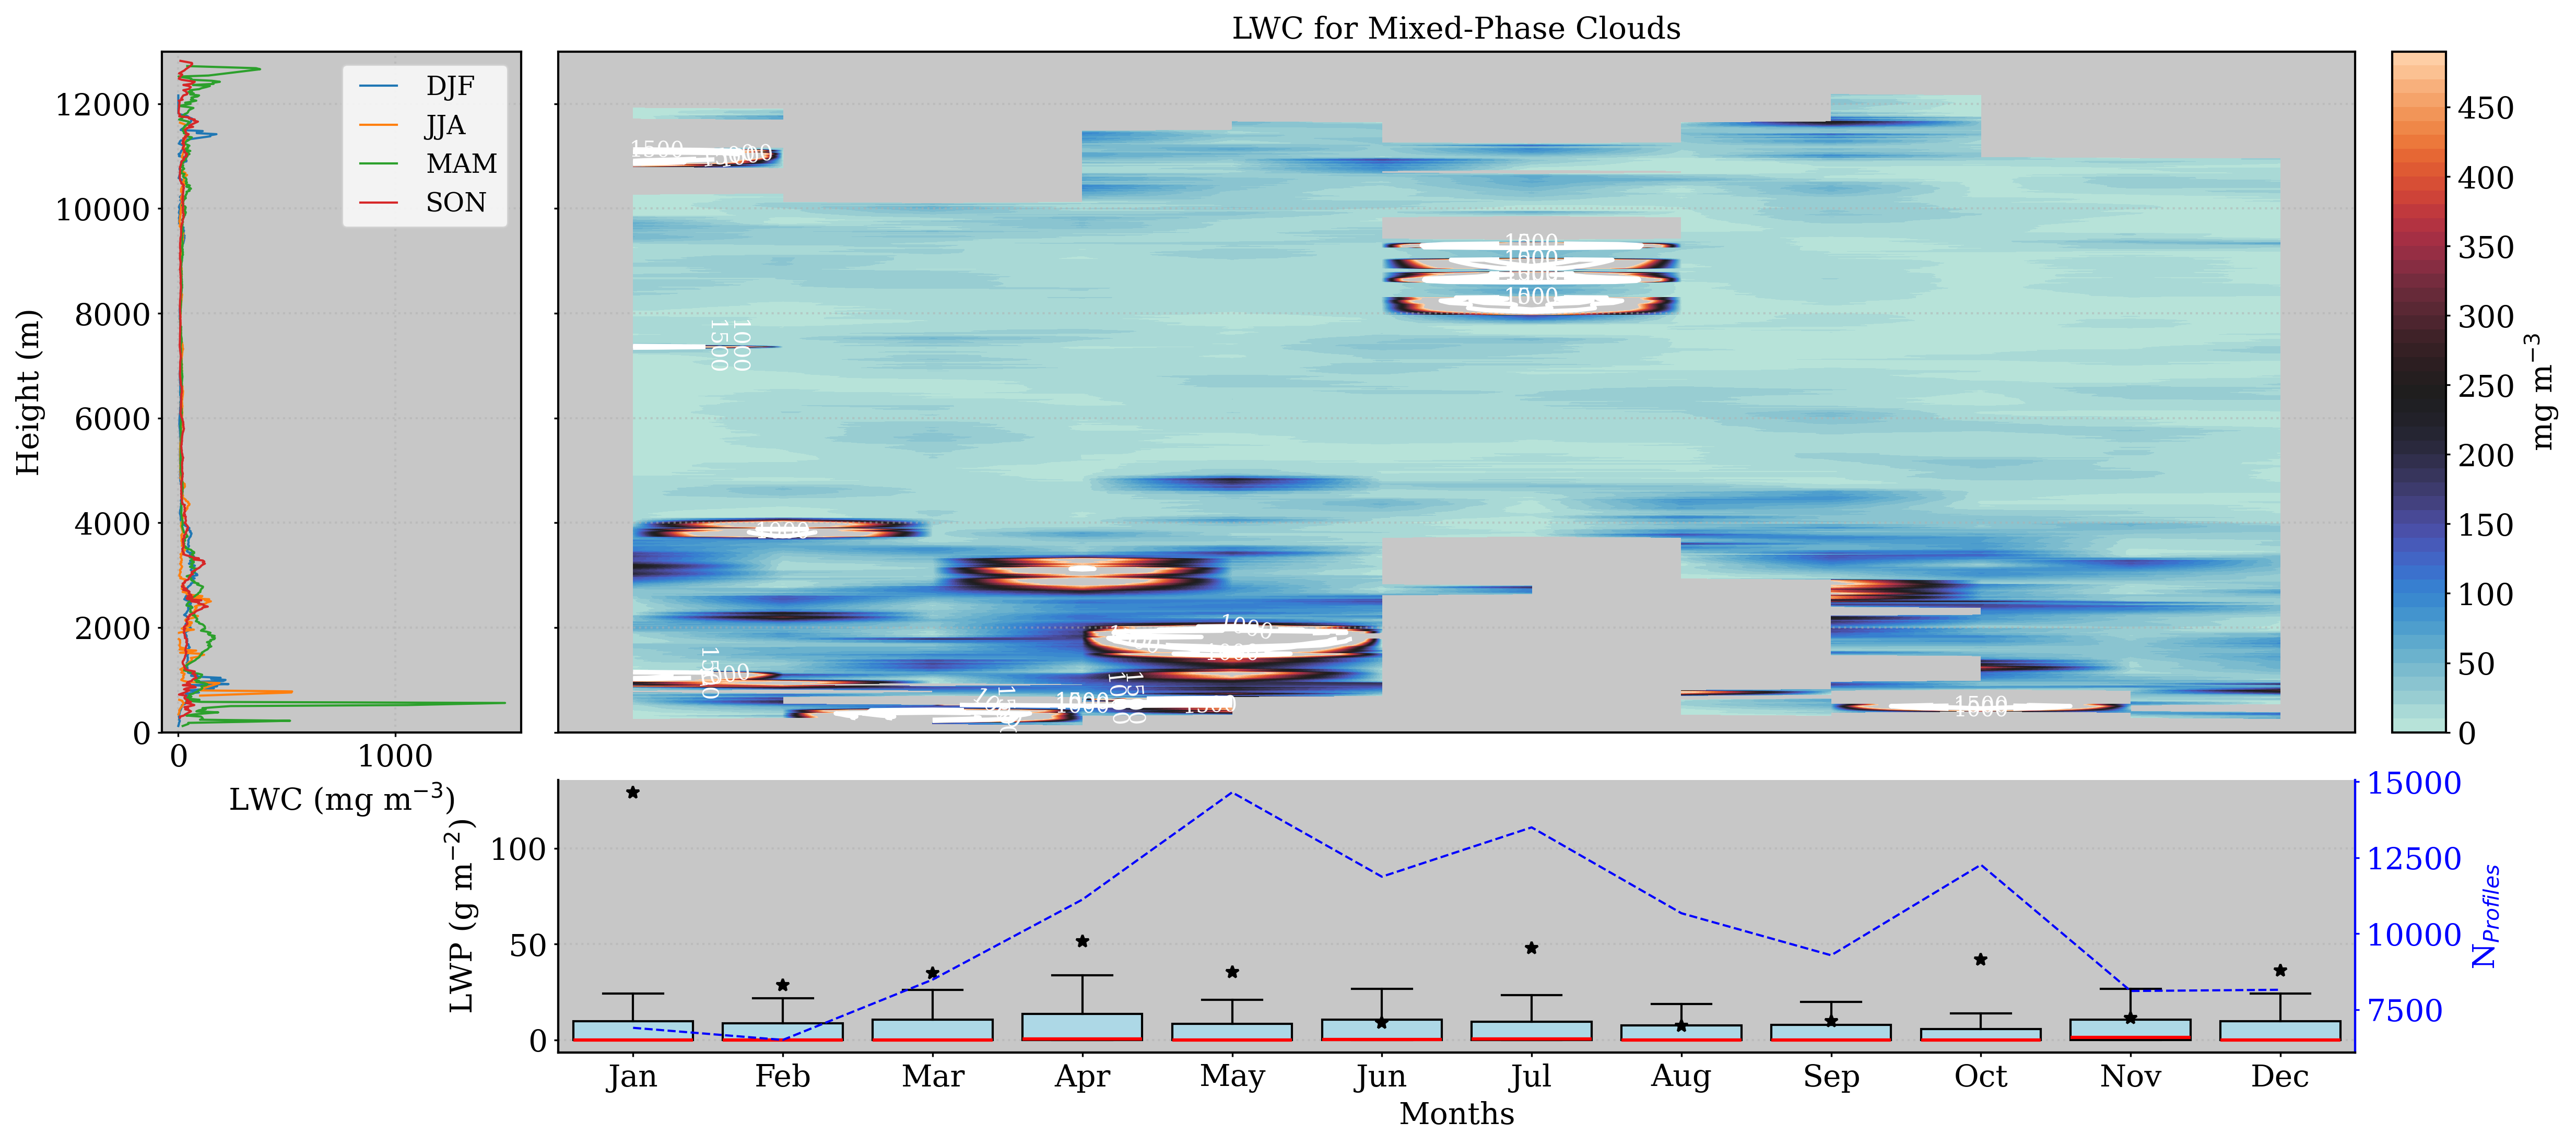
\includegraphics[width=.9\textwidth]{../../phd_clouds/figures/grouped_by_month_evolution_for_lwc_Mixed-Phase_mesh}
	\caption{Same as Figure \ref{fig:LWC_liq}, but for mixed-phase clouds.}
	\label{fig:LWC_mixed}
\end{figure}

In terms of droplet effective radius ($ r_{liq} $), a totally different nature is observed in relation to LWC. The last has expressive amounts of liquid water at low and high layers (< 4 km and > 10 km), while the first is exhibiting high droplet sizes at middle levels. Large values of droplet sizes can be observed on the right-top panel of Figure \ref{fig:DER_mixed} in dark blues and hot tones. They are normally located between 4 and 8 km throughout the entire year, except for July, which also shows larger droplets at 10 km. As already discussed, liquid water is not common at those levels, but when detected, are followed by high mass concentration, suggesting the detection of cumulus clouds. These clouds can have supercooled liquid water at high levels. 

Overall, summer presents higher droplets compared to colder months, with an effective radius between 14-22 $\mu$m at medium heights (> 4 km and < 6 km), and between 12-18$\mu$m around 10 km. On the other hand, droplet sizes are generally close to 10 $\mu$m inside these clouds. This is shown by the monthly distribution of $ r_{liq} $, where the modes are located at even smaller values than the median. In fact, cloud droplets are slightly larger in summer and have a good probability to reach 15 $\mu$m, but in general they present smaller droplets. 

In addition, there is a clear dependency of droplet size with the height. Seasonal profiles on the left panel of Figure \ref{fig:DER_mixed} show droplet size increasing up to 5 km, then starting to decrease. Thus, it is followed by all seasons, indicating that particular seasonal differences of droplet size is only grasped by monthly profile analysis. However, the seasonal profile highlights a general behavior, which can be explained by the ice particle formation. Since temperature decreases with height, ice particles will be formed, increasing the water vapor competition, stopping the process of growing of liquid droplets to form ice particles as temperature continues to decrease. These factors will decrease the size of water droplets and increase the mass concentration of ice particles. The last can be confirmed by the left panel of Figure \ref{fig:IWC_mixed}.

\begin{figure}[H]
	\centering
	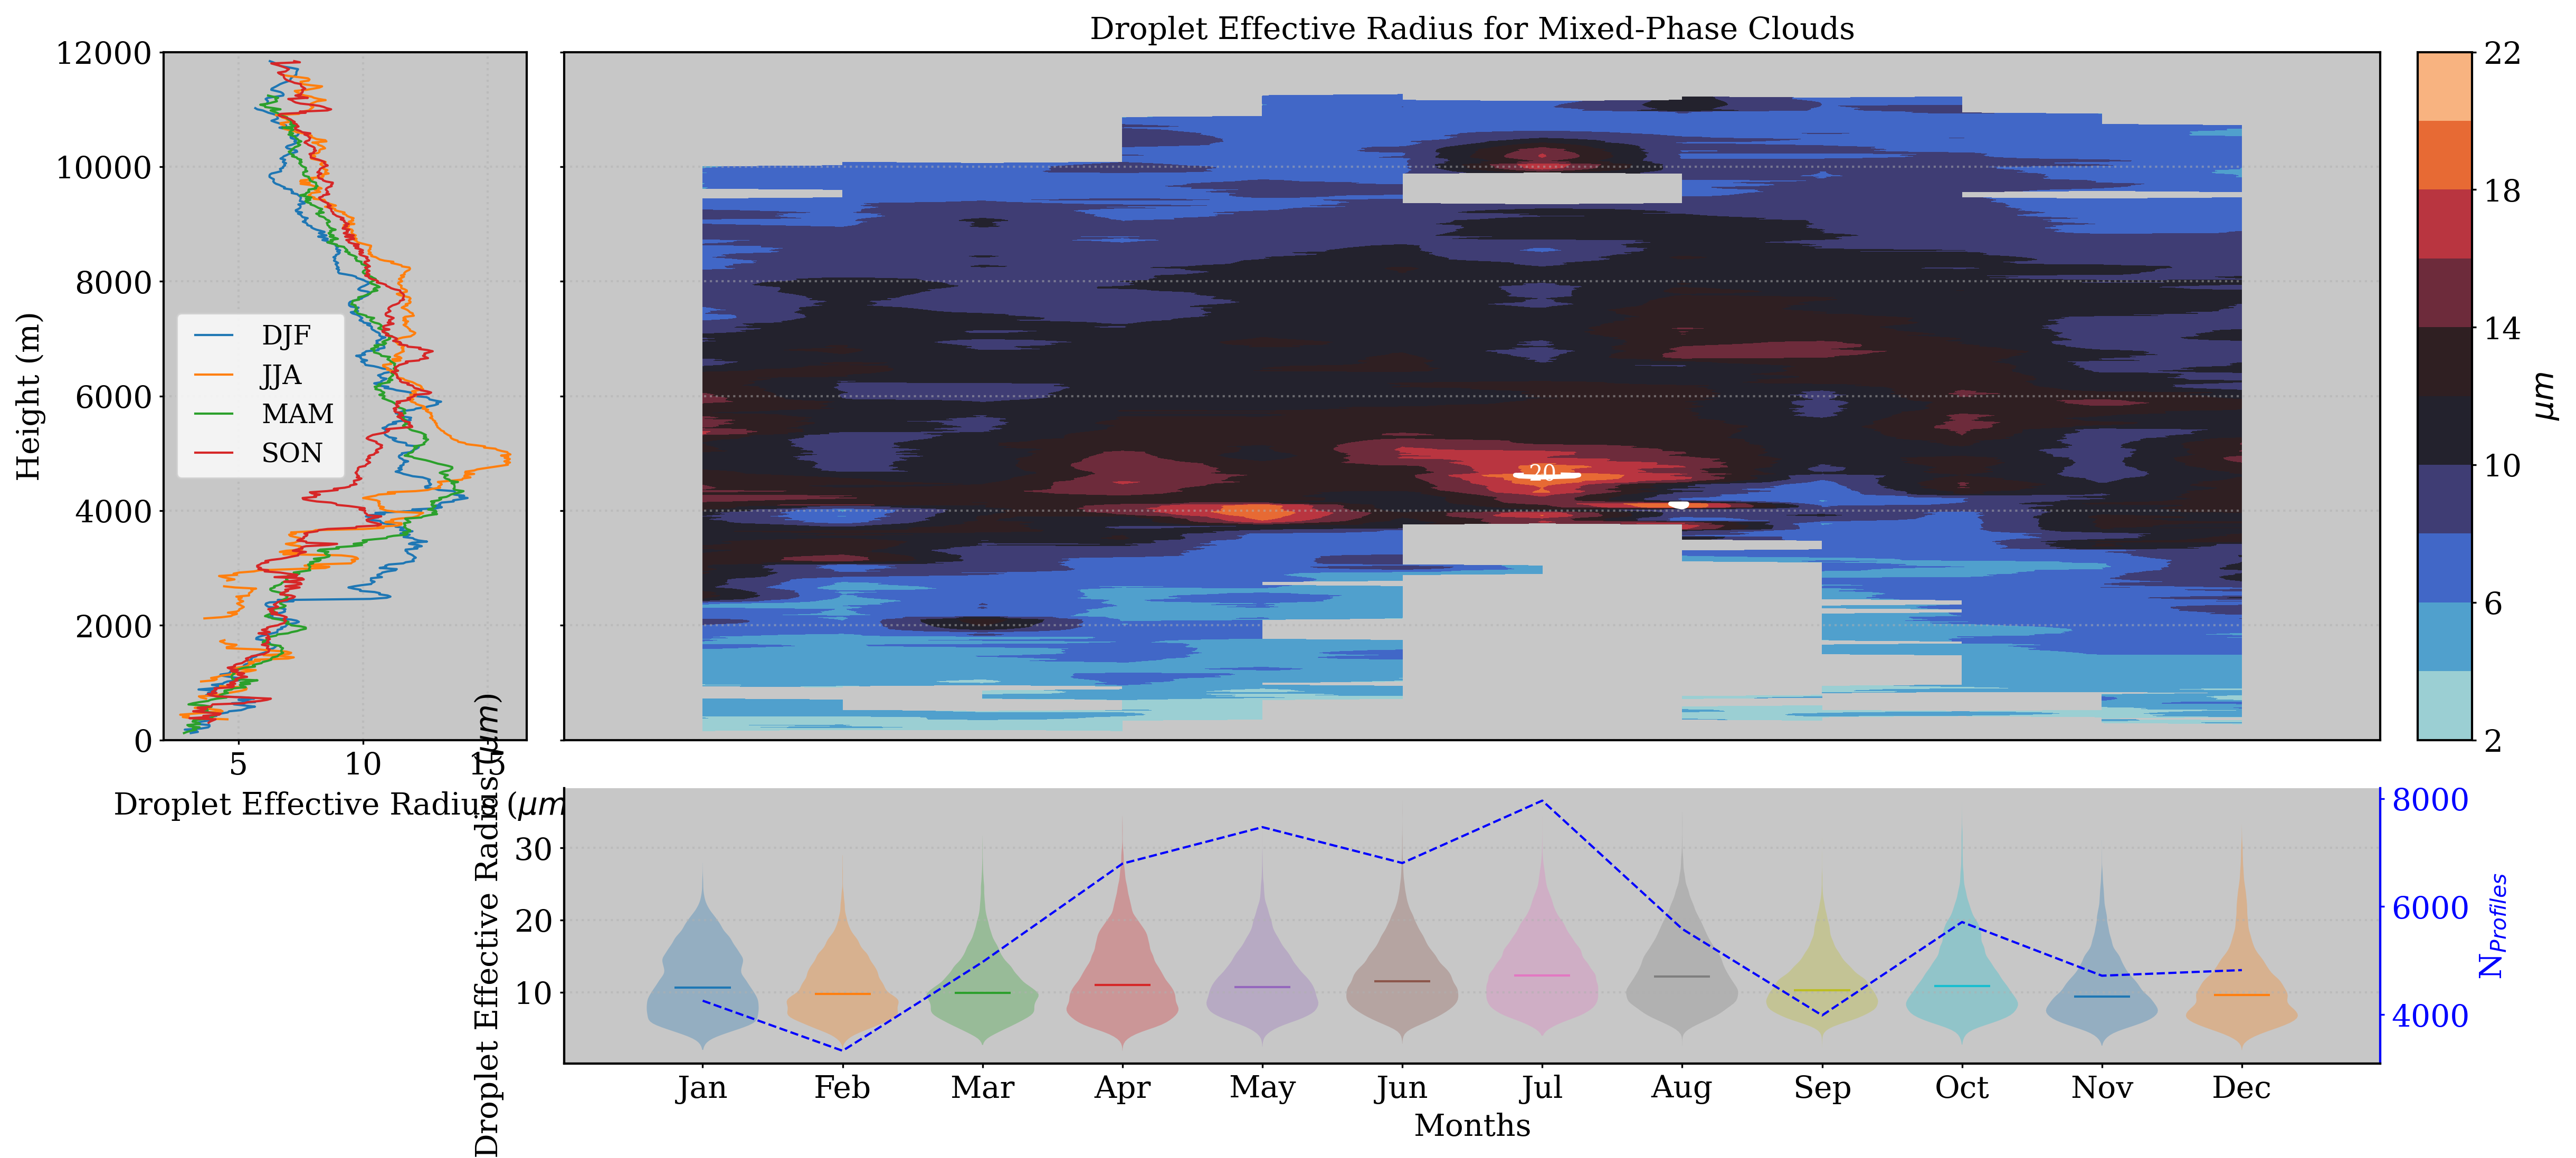
\includegraphics[width=.9\textwidth]{../../phd_clouds/figures/grouped_by_month_evolution_for_der_Mixed-Phase_mesh}
	\caption{Same as figure \ref{fig:DER_liq}, but for mixed-phase clouds.}
	\label{fig:DER_mixed}
\end{figure}

Regarding the ice water content, it exhibits significant variation with height, especially during summer. The monthly median profiles in Figure \ref{fig:IER_mixed} shows that ice mass is greater at middle/high altitudes, as expected. Normally, significant values of IWC of about 20-40 mg m$^{-3}$ are found between 4 and 10 km, except for July. As for the LWC, July also presented elevated IWC above 10 km (more than 60 mg m$^{-3}$), complementing our hypotheses that these clouds can be classified as cumulus clouds. Cumulus clouds are the first stage of cumulonimbus clouds and can have considerable amounts of ice, especially at their top.  In addition, these clouds have a considerable thickness as those observed for mixed phase clouds (some of them can reach 2 km of thickness). 

In terms of IWP, these clouds have low ice amounts as can be seen by the median in the bottom panel, normally below 10 g m$^{-2}$ throughout the entire year. However, the presence of just a few cases with high amounts of ice (outliers) can pull the average up. It happens specially in April and summer, where the physical properties of these clouds are more variable. Also, as already observed, IWC is increasing with altitude, generally formed slightly above 2 km, increasing until 7 km for colder months (winter and spring) and 8 km for warmer months (fall and summer). Winter and fall follow practically the same function of height, as well summer follows the same behavior of fall up to almost 8 km. Above this level, summer has the largest amount of IWC, with maximum, varying between 20 and 10 mg m$^{-3}$.

\begin{figure}[H]
	\centering
	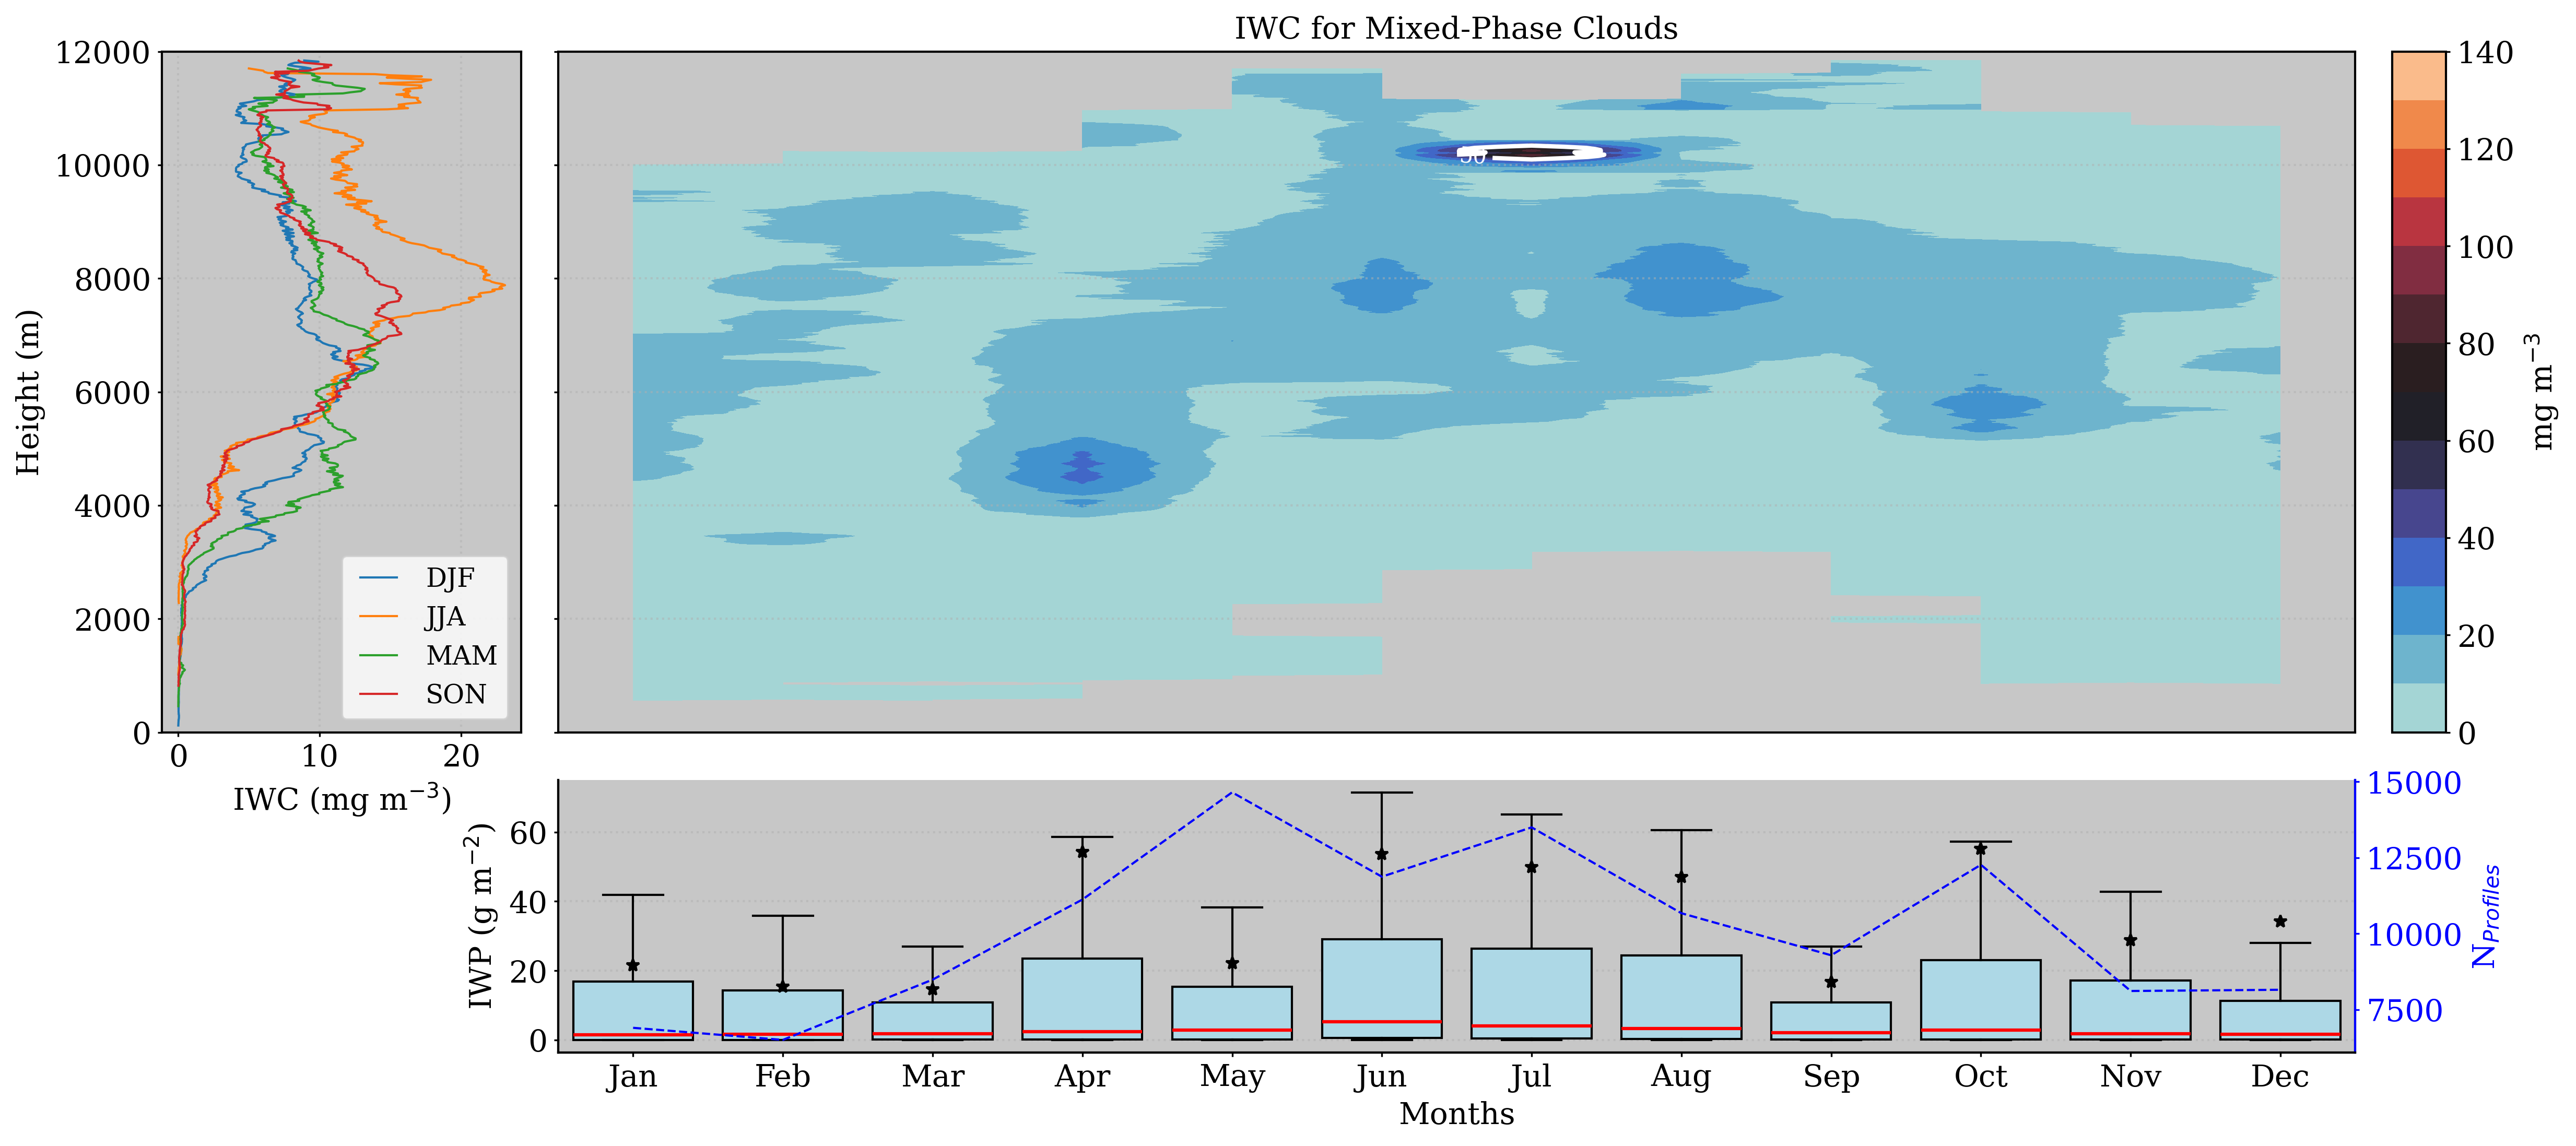
\includegraphics[width=.9\textwidth]{../../phd_clouds/figures/grouped_by_month_evolution_for_iwc_Mixed-Phase_mesh}
	\caption{Seasonal and monthly average of ice water content (IWC) and ice water path (IWP) for mixed-phase clouds. Left panel shows the seasonal median profiles of IWC. 
		%      where the shaded area indicates the standard deviation divided by 10. 
		Right panel shows the monthly median profiles of IWC and monthly box-plot of IWP in the bottom. For the boxplots, medians are denoted by red lines and the average by black stars.}
	\label{fig:IWC_mixed}
\end{figure}

In terms of effective radius, their size follows almost the inverse of the IWC in function of the height. Figure \ref{fig:IER_mixed} undoubtedly shows that higher radii are at low levels, except in July where it's possible to find $ r_{ice} $ larger than 50 $\mu$m above 10 km. Hence, the general properties of these clouds can be described as having larger ice particles with low ice water content (IWC), particularly at lower altitudes. This characteristic is not limited to summer, during which these clouds are distinctly different from those observed throughout the rest of the year. In addition, the monthly distribution (bottom panel of Figure \ref{fig:IER_mixed}) shows that larger ice effective radii are more frequent than small particles. The median is normally fluctuating around 45 $\mu$m, with the mode above this value, indicating high probability of more elevated radius. 
The seasonal profiles (on the left panel of Figure \ref{fig:IER_mixed}) also strengthened our finding that effective radius decreases with height. Actually, it is still almost constant with height up to 6 km, where it starts to decrease. Its values in summer are slightly higher but there are no significant differences over the seasons. Normally, the $ r_{ice} $ is around 30  $\mu$m above 10 km, except for July.

\begin{figure}[H]
	\centering
	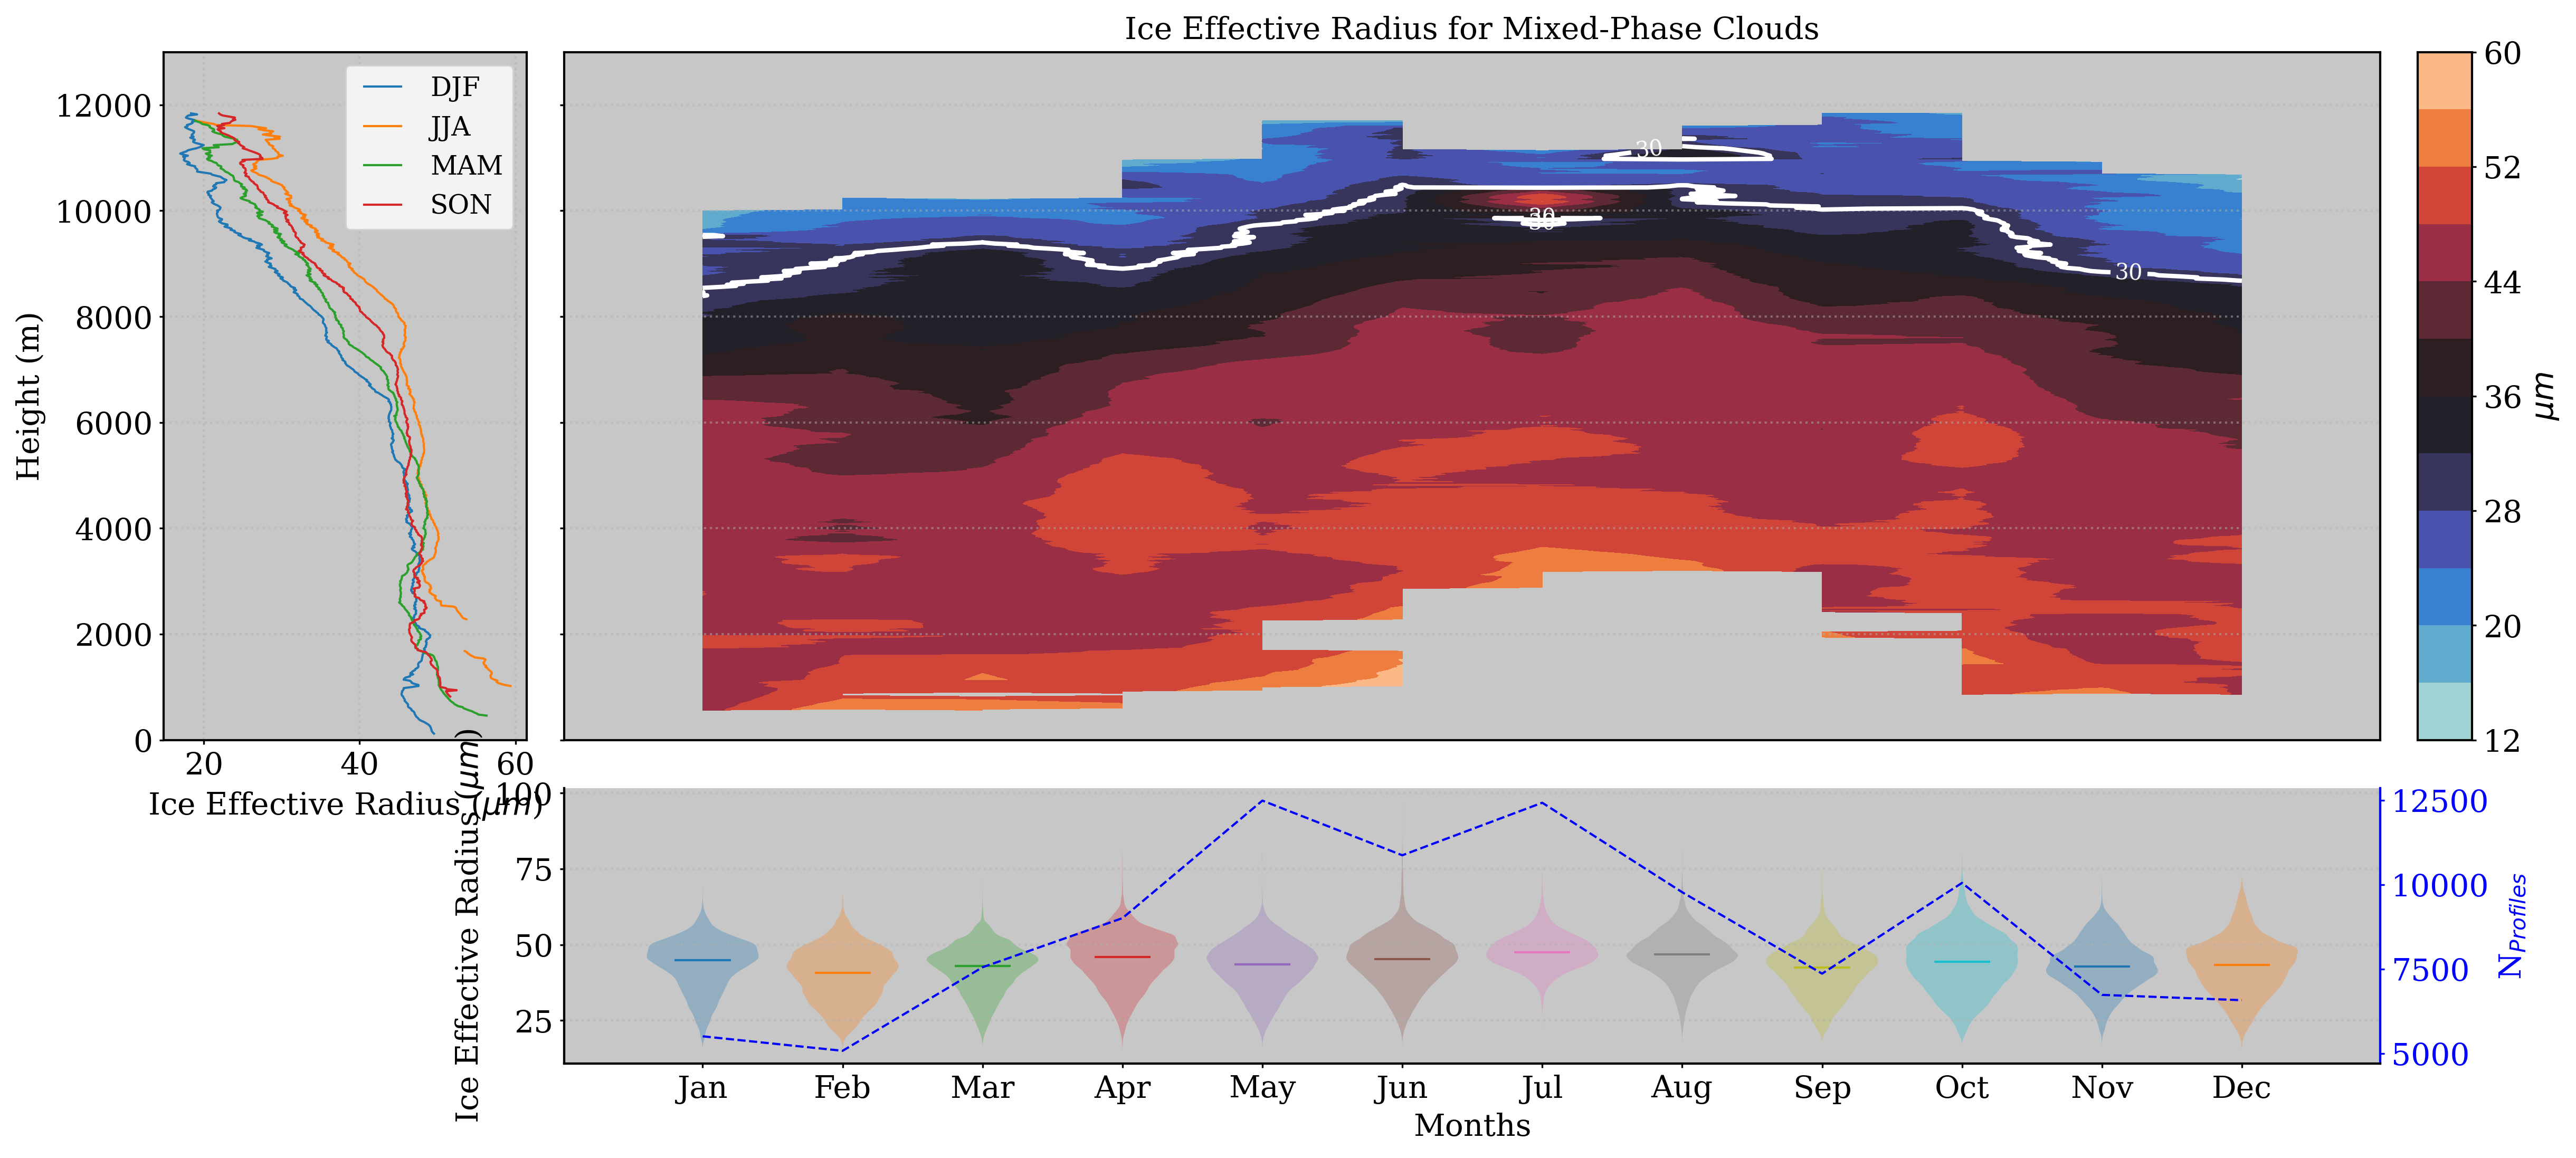
\includegraphics[width=.9\textwidth]{../../phd_clouds/figures/grouped_by_month_evolution_for_ier_Mixed-Phase_mesh}
	\caption{Seasonal and monthly statistics on ice effective radius ($r_{ice}$) distribution for mixed-phase clouds. Left panel shows the seasonal median profiles of ice effective radius. Top-right panel shows the monthly profiles of the median $r_{ice}$, while the bottom-panel displays the size distribution of $r_{ice}$ by months.}
	\label{fig:IER_mixed}
\end{figure}

Regarding the LWC, precipitating mixed-phase clouds follow a similar pattern as non precipitating clouds. However, for the precipitating case, significant amounts of liquid water are located at lower altitudes (< 4km), and they present a stronger seasonal pattern (Top-right panel of Figure \ref{fig:LWC_pre_mixed}). It is natural, considering that we already observed a strong seasonal variability in their frequency of occurrence. In addition, their liquid water content is normally higher than precipitating clouds, as expected. It is worth mentioning that the color scale in Figure \ref{fig:LWC_pre_mixed} is the same as the non precipitating case in Figure \ref{fig:LWC_mixed}, which shows much lighter areas (low values of LWC). Moreover, It is evident that these precipitating clouds do not present such high variability with height, in agreement with their cloud base distribution that showed much less variability than the non precipitating case. Following, winter and spring showed the highest values of LWC, surpassing 1000 mg m$^{-3}$ at some cases close to the surface. These periods show really sharp peaks of LWC, also observed during fall, below 1 km (see left panel). It shows that high concentrations of water in liquid phase are normally found at low levels, following the temperature pattern as expected. It is very known that the temperature at our region significantly increases in summer and fall, allowing liquid cloud droplets to be formed at higher levels. However, these months also have less humidity in the atmosphere, hindering the cloud formation as already observed by the less cloud occurrence.

For summer, a water shortage is clearly observed, especially at low levels. Both in summer and fall (hot months), considerable amounts of LWC are present at medium levels in the atmosphere (> 2 and < 4.5 km). This can be easily seen in the left panel of Figure \ref{fig:LWC_mixed}, where fall (in red) and summer (orange) have almost the same vertical profile, varying around 200 mg m$^{-3}$ between 2 and 4.5 km. At the same layer, the median profile of winter and spring goes through zero at 3 km. Furthermore, the integrated liquid water path has high variability in colder months, with medians below 50 mg m$^{-2}$ and averages above 100 mg m$^{-3}$. In summer, there are just a few occurrences of these clouds, resulting in less variability, with both medians and averages close to zero.

\begin{figure}[H]
	\centering
	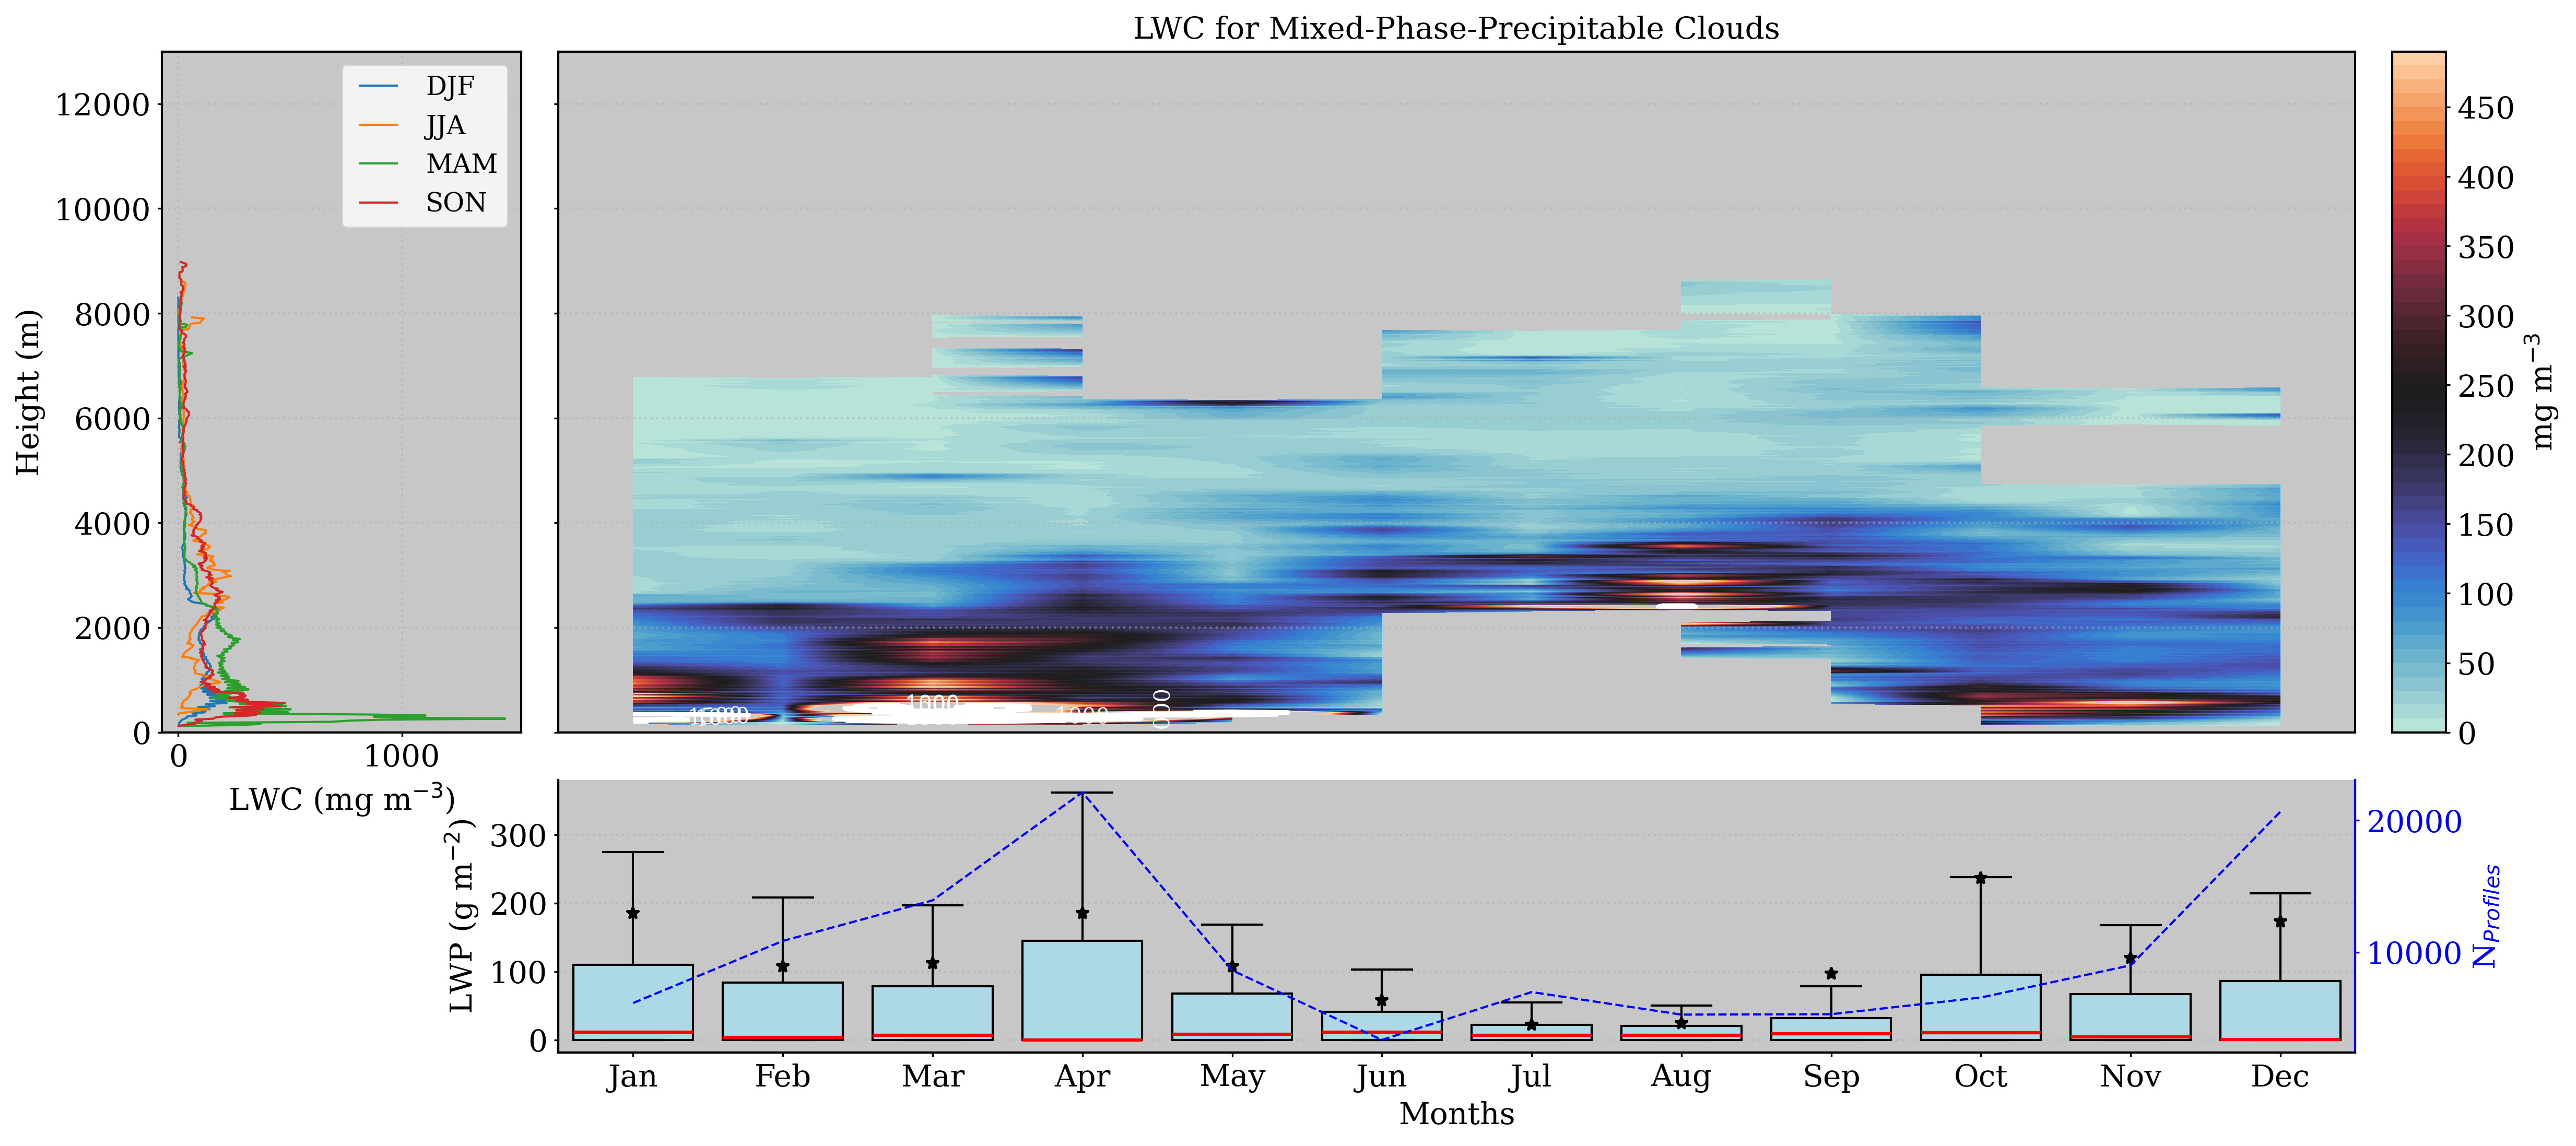
\includegraphics[width=.9\textwidth]{../../phd_clouds/figures/grouped_by_month_evolution_for_lwc_Mixed-Phase-Precipitable_mesh}
	\caption{Same as Figure \ref{fig:LWC_mixed}, but for precipitating mixed-phase clouds.}
	\label{fig:LWC_pre_mixed}
\end{figure}

In relation to the ice effective radius ($r_{ice}$), values below 8 km range from 48 to 64 $\mu$m, with slightly larger particles observed at specific heights during winter and summer—around 5 km in winter and 7 km in summer. Notably, in summer, larger ice particles of 70 $\mu$m can be identified at 10 km, coinciding with higher ice water content (IWC). Such high values can be attributed to strong convective motions, supporting the hypothesis that these summer clouds are cumulonimbus. At the same altitude, $r_{ice}$ values in other months are generally smaller than 30 $\mu$m, except in fall, which also presents higher values at 12 km. Above 1 km, particle size begins to increase (since large particles below are associated with drizzle below the cloud base). For winter and spring, $r_{ice}$ increases up to 5 km (reaching 50 $\mu$m) and then decreases to 20 and 30 $\mu$m, respectively. In contrast, for summer and fall, $r_{ice}$ increases up to 7 km (reaching 50 $\mu$m), then decreases before increasing again to reach second maxima of 50 and 63 $\mu$m, respectively. However, despite the larger variability with height, the monthly distribution of $r_{ice}$ shows a highly variable pattern with a sharp mode at the median position of 50 $\mu$m.

\begin{figure}[H]
	\centering
	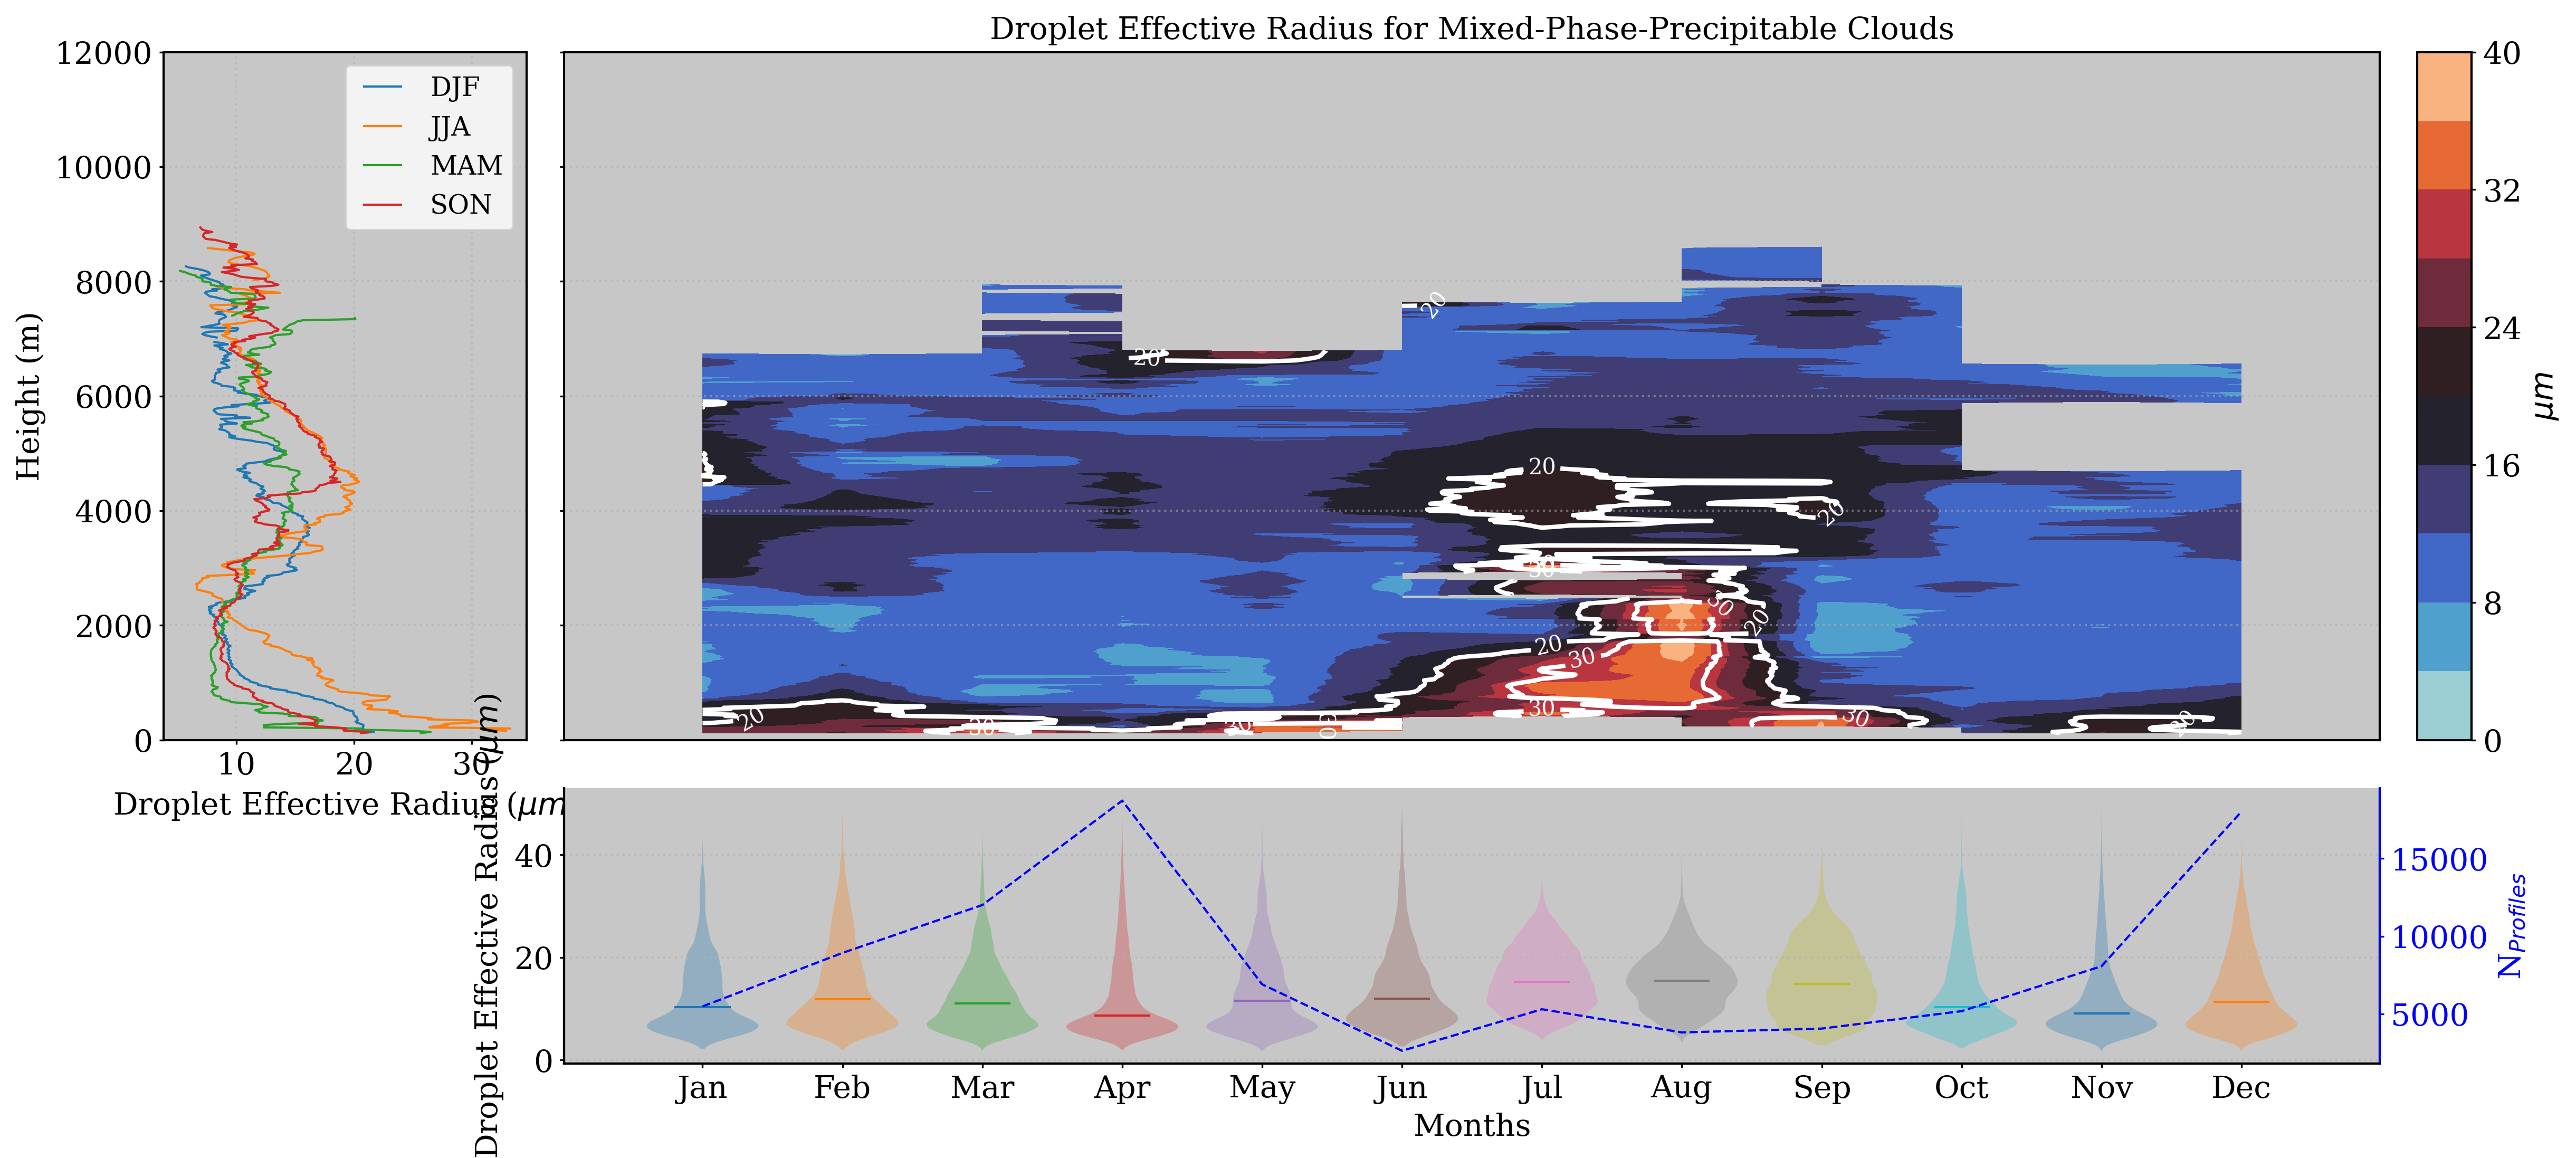
\includegraphics[width=.9\textwidth]{../../phd_clouds/figures/grouped_by_month_evolution_for_der_Mixed-Phase-Precipitable_mesh}
	\caption{Same as figure \ref{fig:DER_mixed}, but for precipitating mixed-phase clouds.}
	\label{fig:DER_pre_mixed}
\end{figure}

Following, Figure \ref{fig:IWC_pre_mixed} reveals that the ice amount inside these clouds is consistently above 3 km, exhibiting high variability with height. The largest amounts of ice water content (IWC) are found during January and November around 5 km, and in June at approximately 8-10 km. However, the median vertical profile by season (left panel of Figure \ref{fig:IWC_pre_mixed}) shows no peaks at these levels for winter, indicating that the high IWC observed in January represents particular cases rather than typical winter conditions. Typically, winter and summer IWC ranges around 20 mg m$^{-3}$ at 3.5 km and fluctuates around 5 mg m$^{-3}$ from 4 km to 9 km.
The low frequency of occurrence of these clouds in summer and fall results in comparable amounts of ice across the months, with fewer outliers. This leads to local maxima in the seasonal profiles of IWC (left panel) that align with the monthly maxima (right panel). Summer shows an almost constant IWC around 20 mg m$^{-3}$ from 5.5 to 7.5 km, with a sharp peak of 200 mg m$^{-3}$ at 9 km. Fall also exhibits IWC around 20 mg m$^{-3}$, but consistently from 5 to 9 km.
Particularly, July, August, and September have the most comparable largest amounts of IWC in the atmosphere. Consequently, the 25th, 50th, and 75th percentiles during these months are relatively higher, with 25\% of the data showing IWC values exceeding 200 mg m$^{-2}$.

\begin{figure}[H]
	\centering
	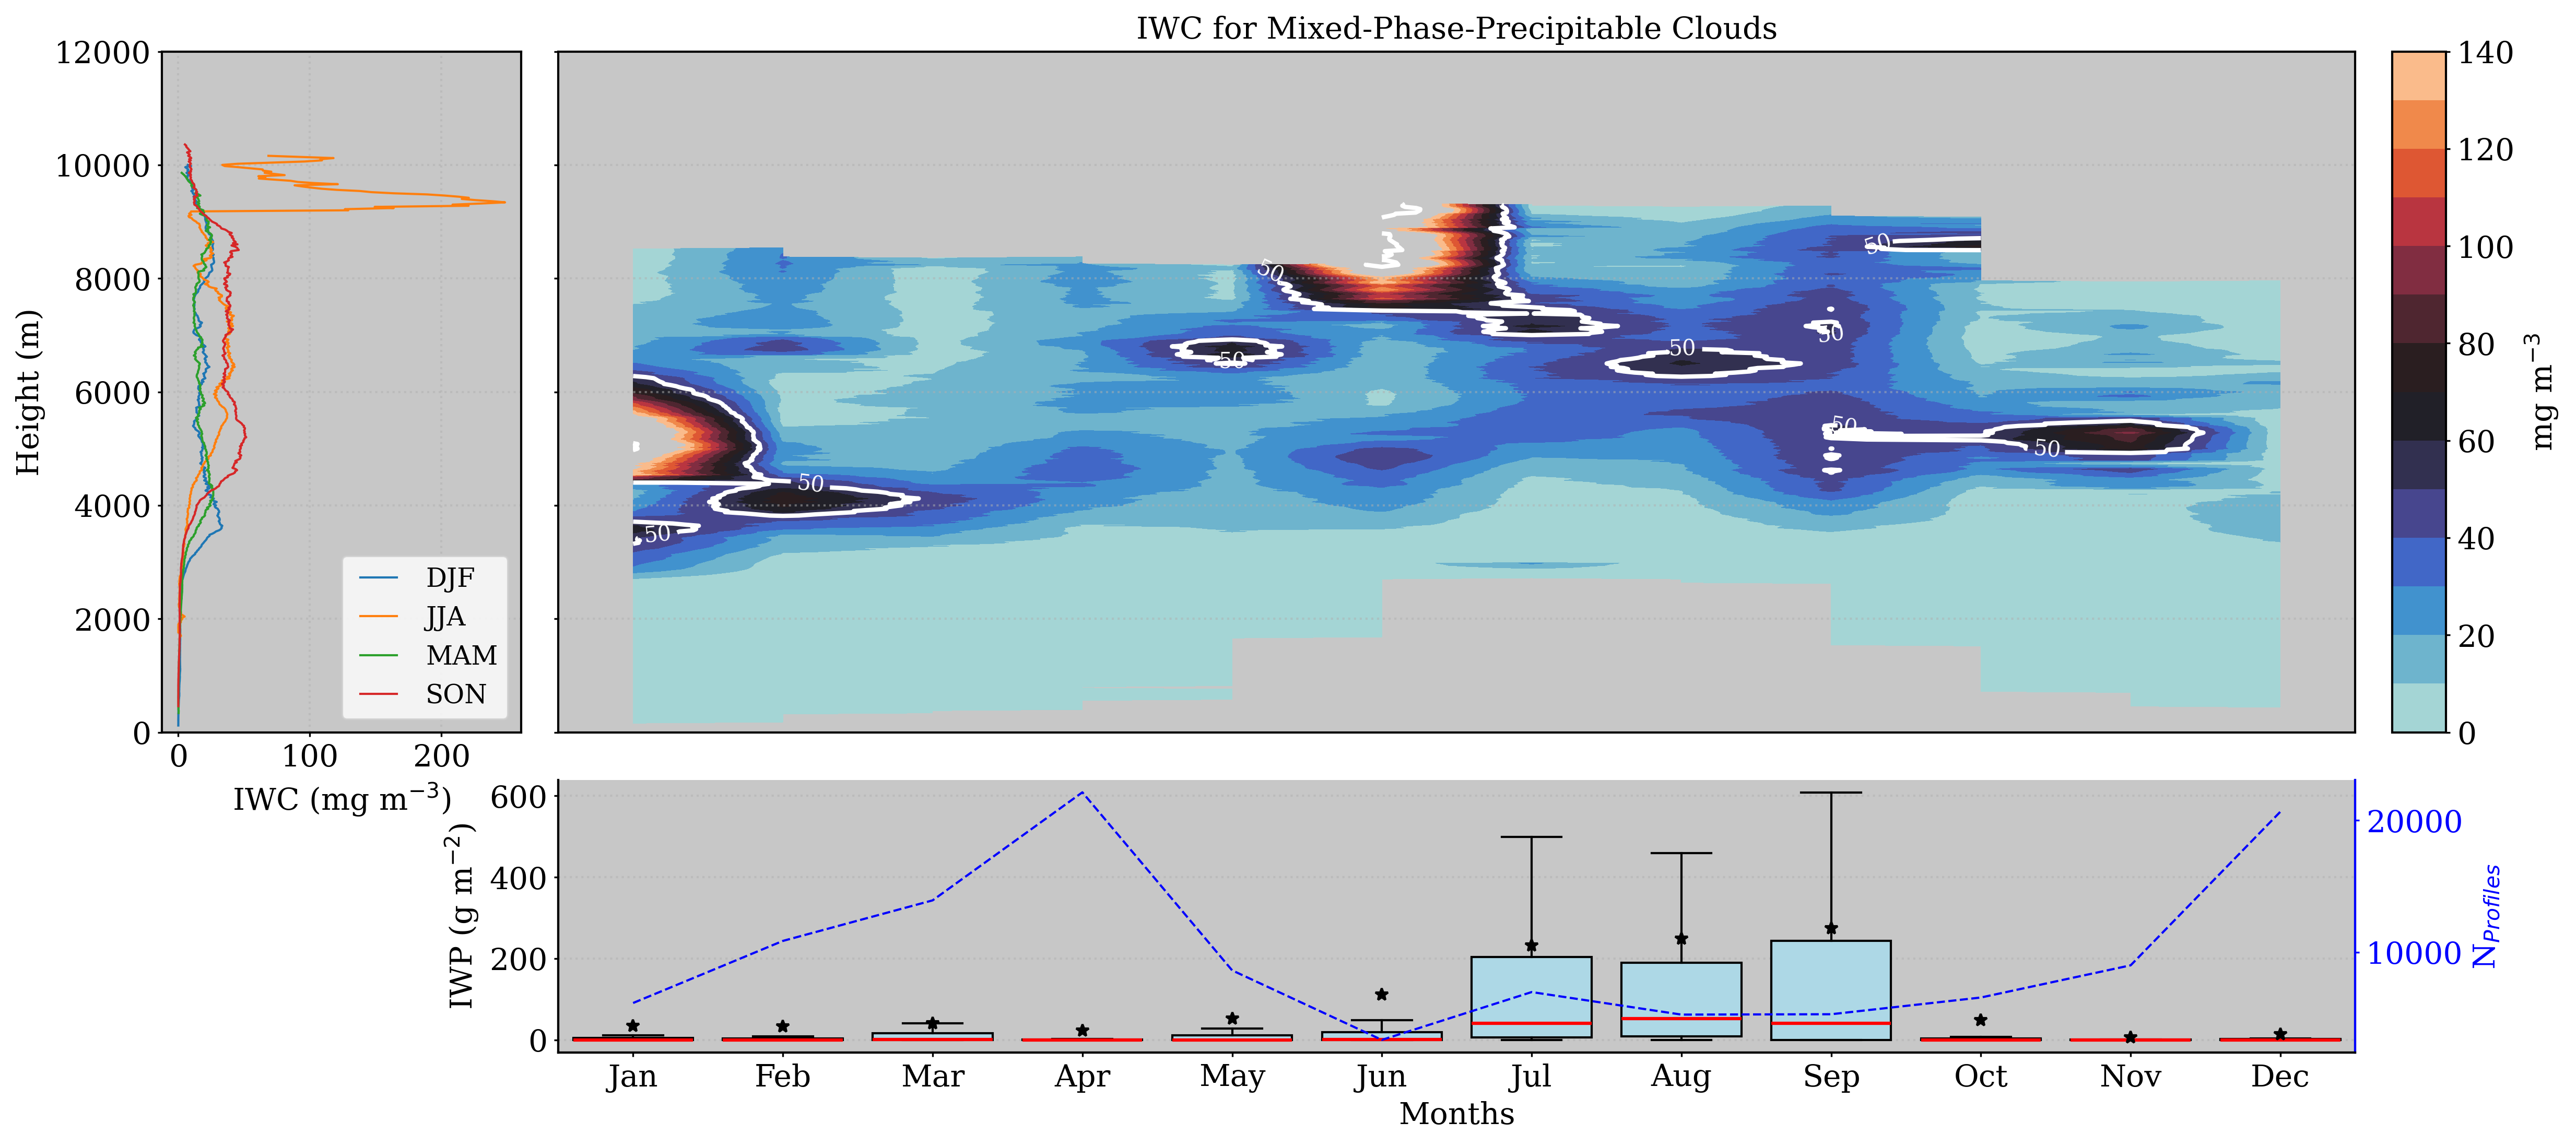
\includegraphics[width=.9\textwidth]{../../phd_clouds/figures/grouped_by_month_evolution_for_iwc_Mixed-Phase-Precipitable_mesh}
	\caption{Same as Figure \ref{fig:IWC_mixed}, but for precipitating mixed-phase clouds.}
	\label{fig:IWC_pre_mixed}
\end{figure}

In terms of effective radius, the largest values are found below 8 km, with the highest values occurring in summer and fall (dark red), as shown in Figure \ref{fig:IER_pre_mixed}. During these months, ice particle sizes exhibit less variability with height, ranging around 50-55 $\mu$m. Conversely, winter and spring show variability between 45 and 55 $\mu$m. The left panel of Figure \ref{fig:IER_pre_mixed} clearly separates warm months (summer-fall) from colder months (winter-spring).
In warm months, the ice effective radius remains almost constant around 50 $\mu$m up to 8 km. Above this altitude, particle sizes decrease in fall, while summer exhibits a sharp maximum at 9 km, coinciding with the maximum IWC region. Winter and spring also have similar $r_{ice}$ values to those in summer and fall up to 4 km, after which the sizes decrease with height, reaching 20 $\mu$m at 10 km.
Despite this variability of $r_{ice}$ with height, the monthly distribution shows that within these clouds, $r_{ice}$ is generally around 55 $\mu$m.

\begin{figure}[H]
	\centering
	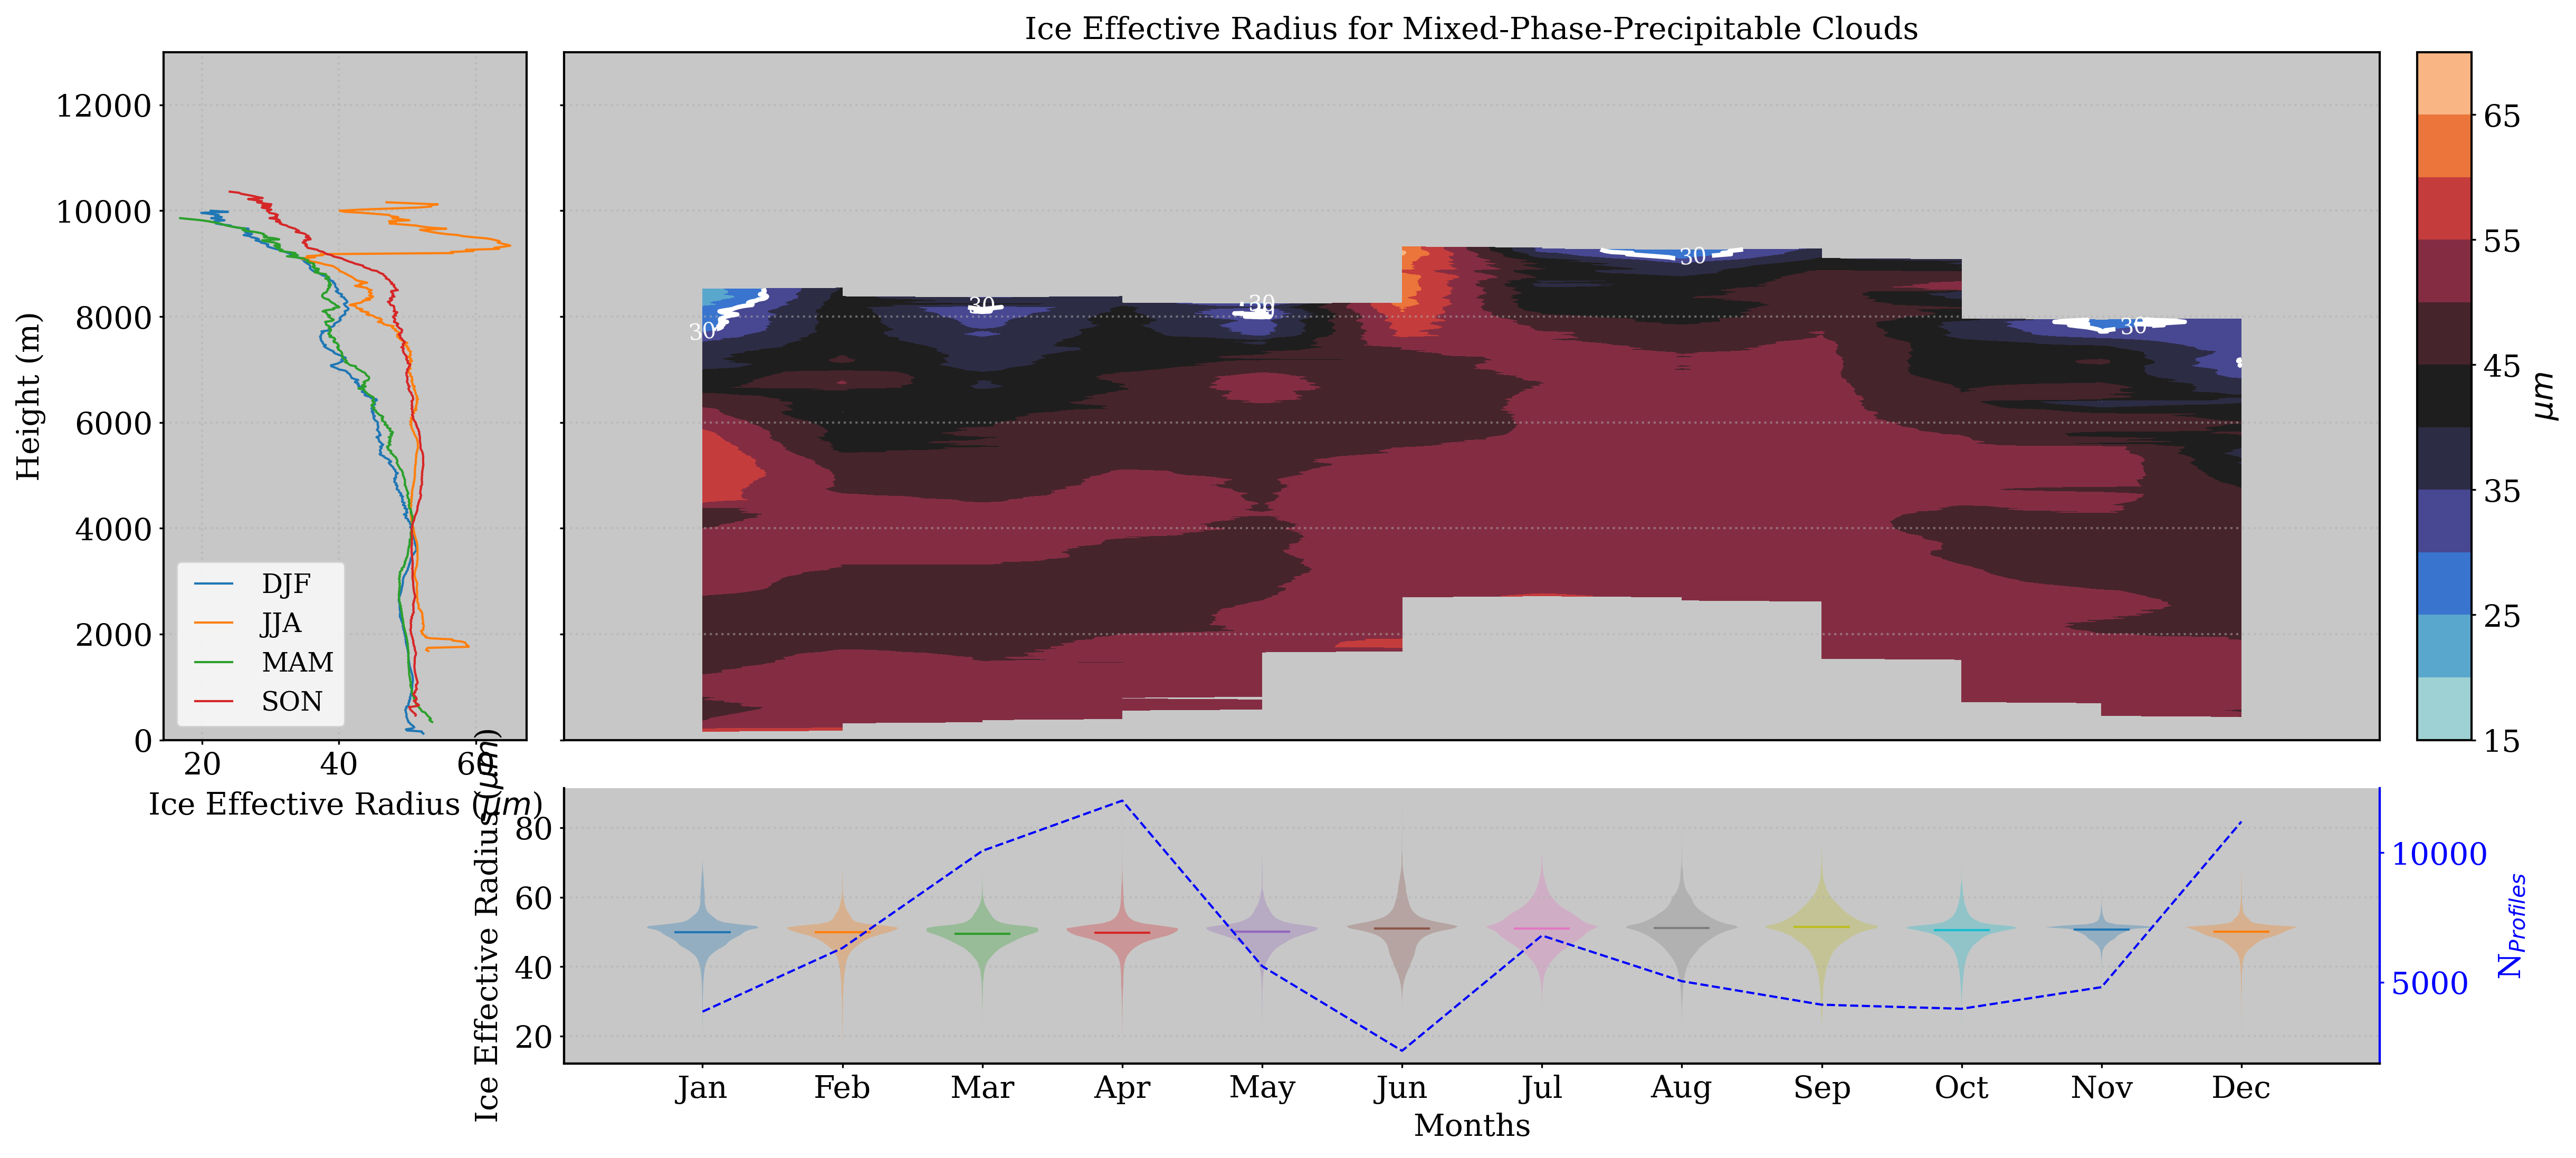
\includegraphics[width=.9\textwidth]{../../phd_clouds/figures/grouped_by_month_evolution_for_ier_Mixed-Phase-Precipitable_mesh}
	\caption{Same as figure \ref{fig:IER_mixed}, but for precipitating mixed-phase clouds.}
	\label{fig:IER_pre_mixed}
\end{figure}

Overall, Mixed-phase clouds exhibit less liquid water content (LWC) than liquid clouds. Typically, the LWC in liquid clouds is concentrated at low levels, with some exceptions in June and July, where high LWC values are observed above 8 km. Mixed-phase clouds also contain less ice water content (IWC) compared to ice clouds, with the IWC found at higher altitudes due to dependency on low temperatures, leading to elevated IWC levels higher in the atmosphere during summer. The droplet effective radius in mixed-phase clouds is larger at mid-levels, while the ice effective radius is larger at mid-levels during winter and spring and around 8 km during fall and summer. Unlike this pattern, the ice effective radius in these clouds slightly decreases with height up to 6 km, where the rate of decrease intensifies. Precipitating mixed-phase clouds exhibit a stronger seasonal profile, with higher LWC, particularly in spring and fall at lower levels. They also show significantly more IWC in summer and early fall. The droplet effective radius ($r_{liq}$) in precipitating mixed-phase clouds is typically higher than in mixed-phase clouds, especially near the surface and at mid-levels, due to the presence of drizzle particles at low levels. In terms of the ice effective radius ($r_{ice}$), these clouds display a clear seasonal variation, with higher $r_{ice}$ values in summer and fall above 4 km. Additionally, precipitating clouds show larger IWC and $r_{ice}$ values at 9 km in summer, suggesting a possible association with cumulus clouds.


\subsubsection{Ice Clouds}

The ice water content (IWC) of ice clouds exhibits clear seasonal patterns, as evident from Figure \ref{fig:IWC_ice}. The smallest ice amounts are observed in summer, particularly in July, coinciding with the minimum frequency of ice cloud occurrence. In contrast, the highest IWC values, exceeding 50 mg m$^{-3}$, are found at altitudes of 4-6 km in June and October, and near the ground in January. Typically, these clouds are situated higher in the atmosphere, with cloud bases around 7-8 km, with only 25\% of ice clouds having bases below 6 km. These lower clouds generally contain the largest ice amounts, ranging between 30 and 100 mg m$^{-3}$, except in January. Notably, January exhibits much higher IWC near the ground, an anomaly attributed to extreme weather events such as the Filomena storm in 2020 and the Gloria storm in 2021, which significantly impacted the western Mediterranean region \citep{samuelt.buisanAdjustmentSolidPrecipitation2022,mariaeugeniaperez-gonzalezEvaluationImpactCaused2022,martadealfonsoStormGloriaSea2021}. Conversely, clouds above 8 km, often associated with cirrus clouds, typically have much lower ice content, ranging from 0 to 20 mg m$^{-3}$, except in fall, where clouds with IWC around 50 mg m$^{-3}$ are observed at 12 km. These seasonal variations are also evident in the left panel of Figure \ref{fig:IWC_ice}, which shows substantial ice near the surface in winter. This was already identified as the influence of  two snowfall events, resulting in a median IWC of 400 mg m$^{-3}$ around 1 km. The variability compared to other years without such high IWC values is highlighted in the bottom panel of Figure \ref{fig:IWC_ice}, where the average liquid water path (LWP) is much higher than the median for January, indicating that typical IWP values for January are low, around 10 mg m$^{-2}$. Overall, the monthly IWP distributions for ice clouds are relatively consistent throughout the year, indicating a well-defined annual IWP pattern, except in January and July. January shows lower occurrence rates and is impacted by the snowfall events, while July is characterized by an extremely low occurrence of ice clouds, resulting in a minimum LWP.

\begin{figure}[H]
	\centering
	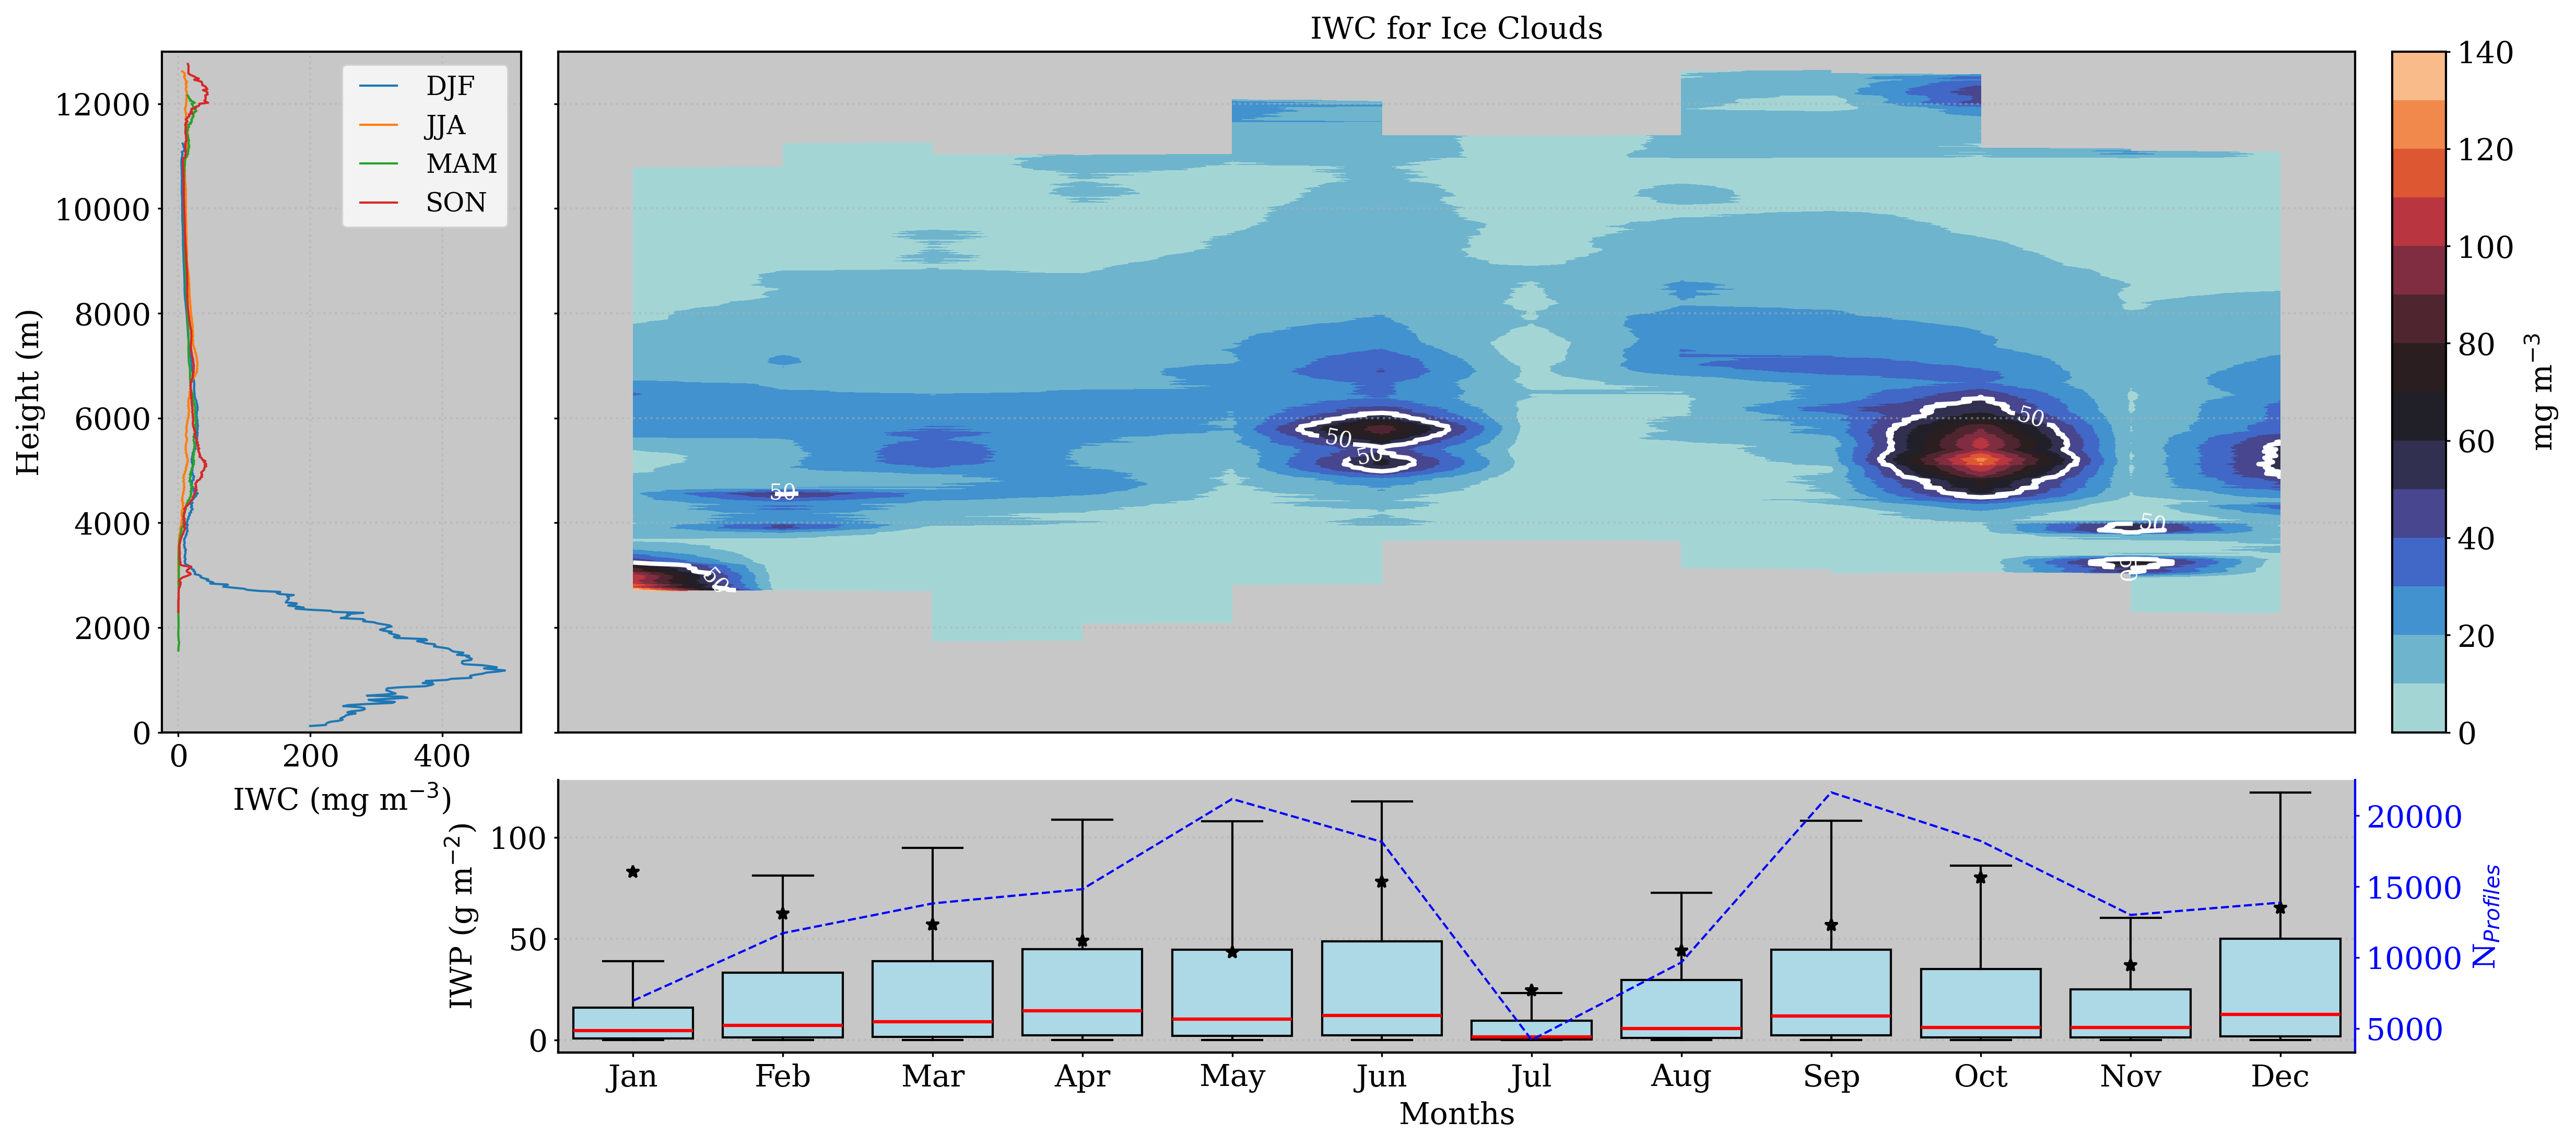
\includegraphics[width=.9\textwidth]{../../phd_clouds/figures/grouped_by_month_evolution_for_iwc_Ice_mesh}
	\caption{Seasonal and monthly average of ice water content (IWC) and ice water path (IWP) for ice clouds. Left panel shows the seasonal median profiles of IWC. 
		%      where the shaded area indicates the standard deviation divided by 10. 
		Right panel shows the monthly median profiles of IWC and monthly box-plot of IWP in the bottom. For the boxplots, medians are denoted by red lines and the average by black stars.}
	\label{fig:IWC_ice}
\end{figure}

In terms of ice effective radius, their size is also larger at middle levels, ranging around 50 and 60 $\mu$m. In addition, January also presented elevated $r_{ice}$ closer to the ground (clearly seen in the left panel of figure Figure \ref{fig:IER_ice}), as a result of the snowfalls. However, beyond this month, the maximum size of 60 $\mu$m is normally observed exclusively in June and October in mid levels. Left panel of Figure \ref{fig:IER_ice} shows that above 6 km, ice particle size diminishes, indicating a larger cloud radius at lower levels, a pattern also observed in mixed-phase clouds. Typically, ice particles are larger at low and mid-levels, except in clouds with significant convective activity, such as cumulus and cumulonimbus clouds. Cirrus clouds situated above 8 km have an ice effective radius between 40 and 45 $\mu$m, decreasing with altitude up to 11 km. At this level, during spring and summer, these clouds reach 25 $\mu$m, while in winter, the size reduces to 20 $\mu$m (see Left panel of Figure \ref{fig:IER_ice}). In fall, a slight increase in size is observed at 12 km, coinciding with high IWC levels, linked to cirrus clouds with higher ice crystal concentrations. The monthly distribution reveals a stable median ice particle size of approximately 38 $\mu$m throughout the year, indicating that this value is generally representative when considering all radii within the atmosphere for this cloud type. However, January presents a distribution with a new mode around 50 $\mu$m, as expected due to the snowfall events already discussed. 

\begin{figure}[H]
	\centering
	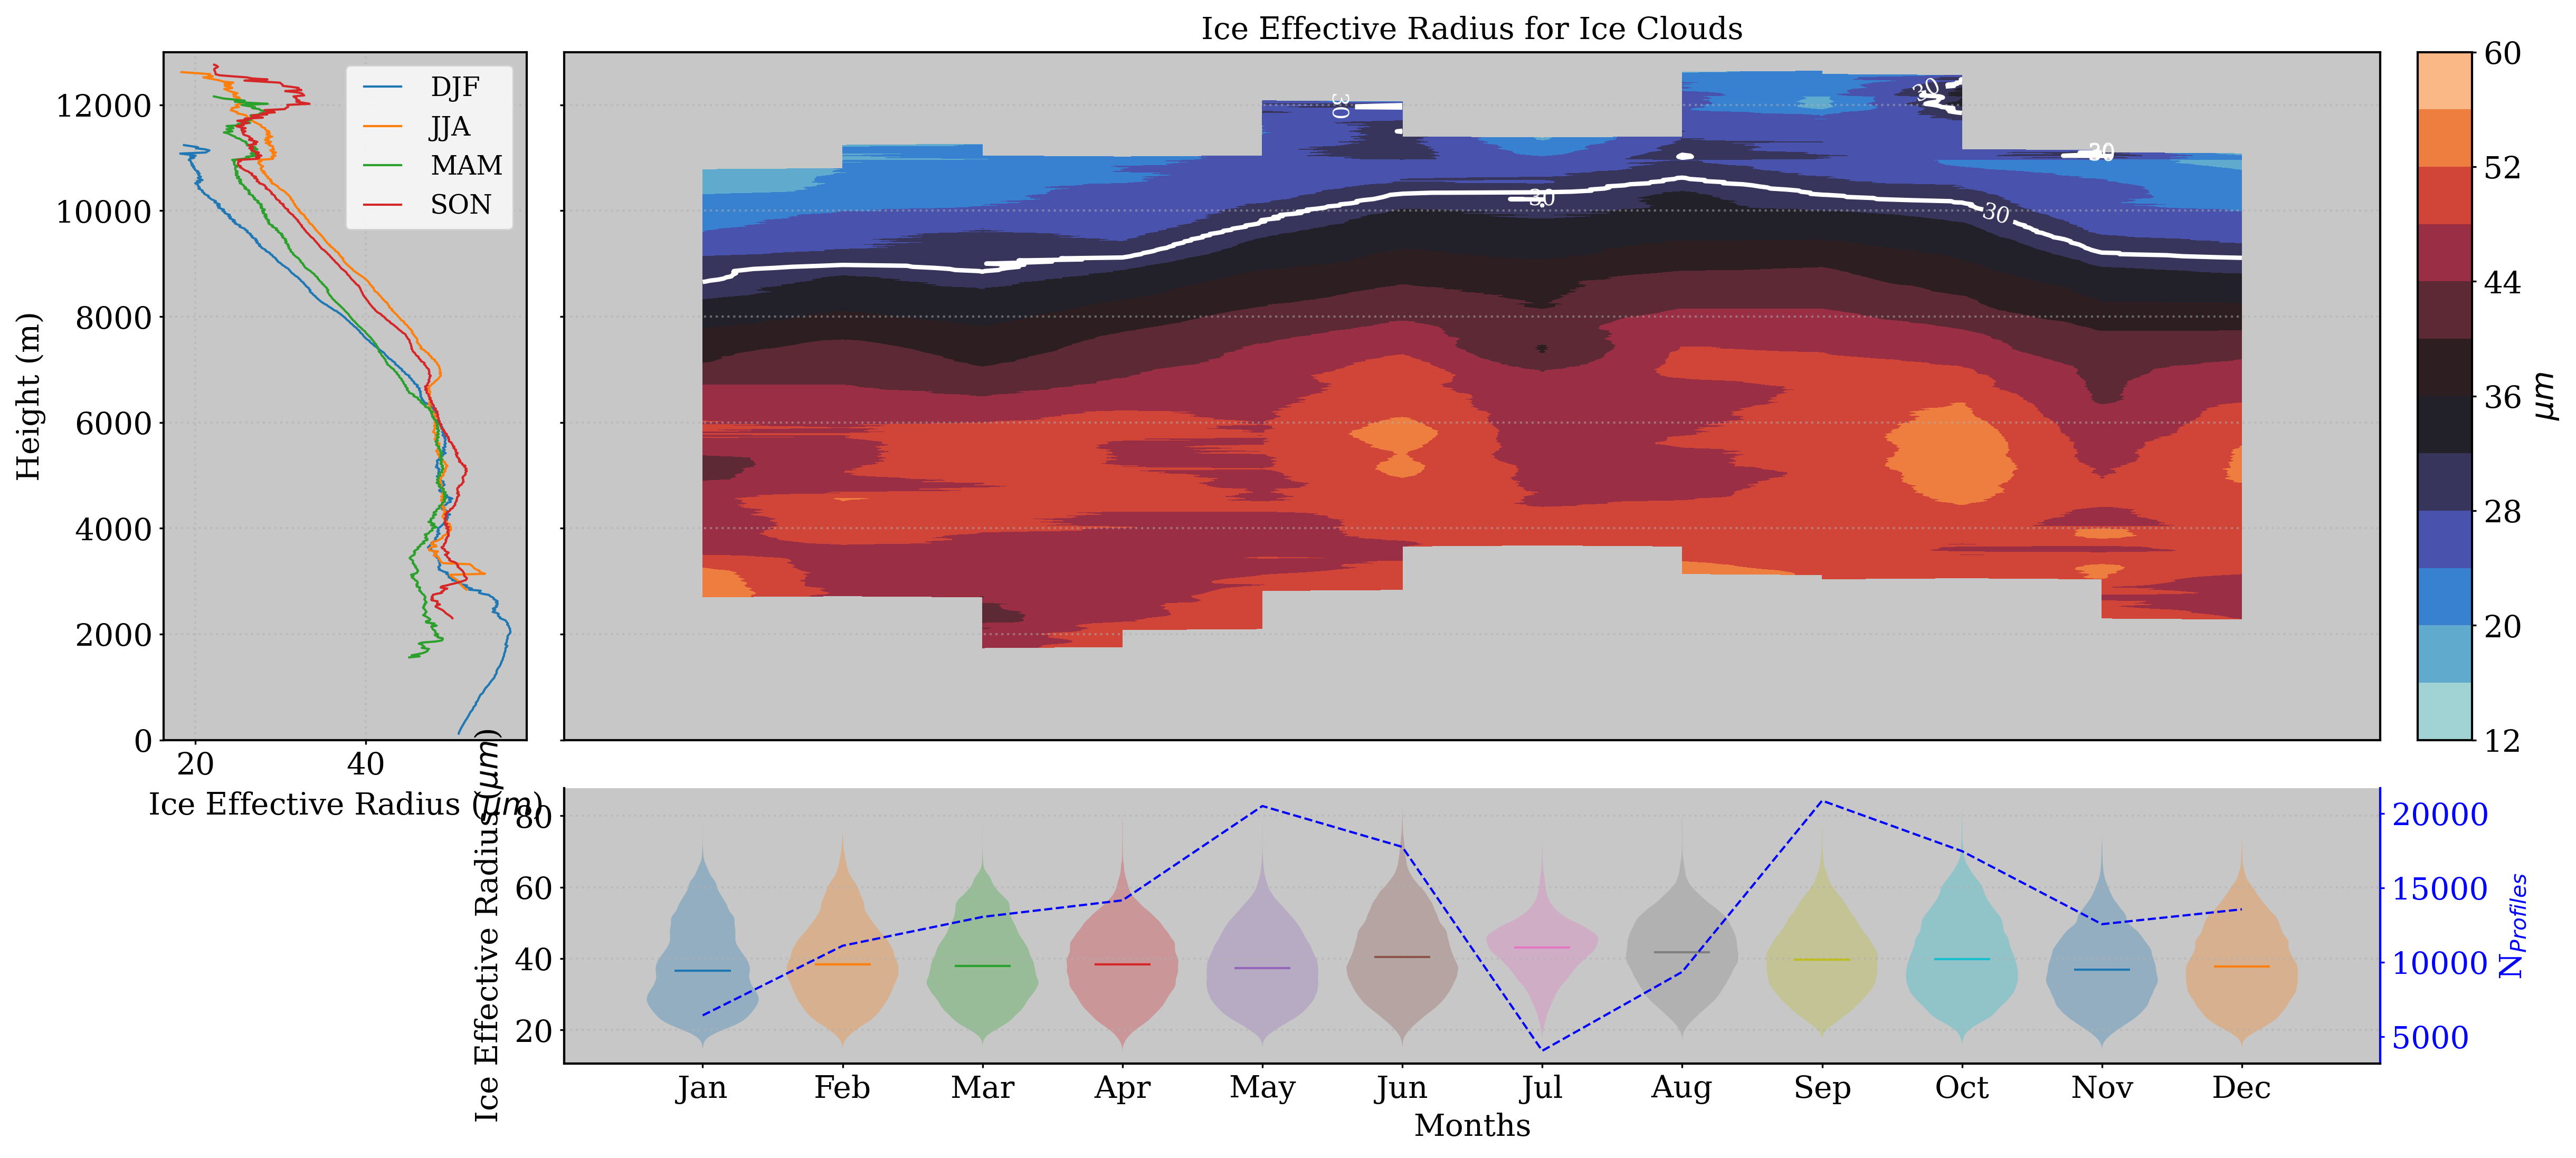
\includegraphics[width=.9\textwidth]{../../phd_clouds/figures/grouped_by_month_evolution_for_ier_Ice_mesh}
	\caption{Seasonal and monthly statistics on ice effective radius ($r_{ice}$) distribution for ice clouds. Left panel shows the seasonal median profiles of ice effective radius. Top-right panel shows the monthly profiles of the median $r_{ice}$, while the bottom-panel displays the size distribution of $r_{ice}$ by months.}
	\label{fig:IER_ice}
\end{figure}

Ice precipitating clouds are the most frequent at our station, characterized by their greater thickness and lower cloud base compared to non-precipitating ice clouds. Similar to precipitating mixed-phase clouds, these clouds possess a well-defined melting layer that separates the cloud base from rain droplets and drizzle. The highest concentrations of ice, exceeding 50 mg m$^{-3}$, are found between 2 and 5 km, with slightly elevated levels during summer and fall. Notably, regions with ice concentrations over 200 mg m$^{-3}$ were identified around 6 km in June and September, and between 9 and 12 km in July. This significant ice presence at high altitudes was not observed in ice clouds, though a relatively high ice content was detected in precipitating mixed-phase clouds in June, suggesting a correlation with the high ice amounts in summer and thicker clouds. The substantial ice amounts at high altitudes in summer are strongly linked to convective motions, providing evidence that precipitating ice clouds in summer may be associated with cumulonimbus clouds. Additionally, these clouds may represent a subsequent stage of precipitating mixed-phase clouds, exhibiting a similar pattern but with increased thickness and ice water content, particularly in summer. The left panel of Figure \ref{fig:IWC_ice_prep} illustrates similar median profiles of IWC in summer and fall, with summer displaying a secondary maximum around 11 km and fall showing a more pronounced second maximum at 13 km. In contrast, spring and winter exhibit similar maxima of 100 and 150 mg m$^{-3}$ around 4.5 km, respectively, slightly below the primary maxima of 200 mg m$^{-3}$ observed in summer and fall around 6 km. The bottom panel of Figure \ref{fig:IWC_ice_prep} highlights that these clouds contain significantly higher ice water content compared to other clouds, especially during summer and fall, with the 75th percentile increasing from 500 to 1000 mg m$^{-2}$. Furthermore, it is noteworthy that the IWP in other months is much lower, indicating that in months with a higher occurrence of these clouds, the IWP is more variable and generally smaller. The lower occurrence of warm clouds results in comparable IWC values and reduced variability.


\begin{figure}[H]
	\centering
	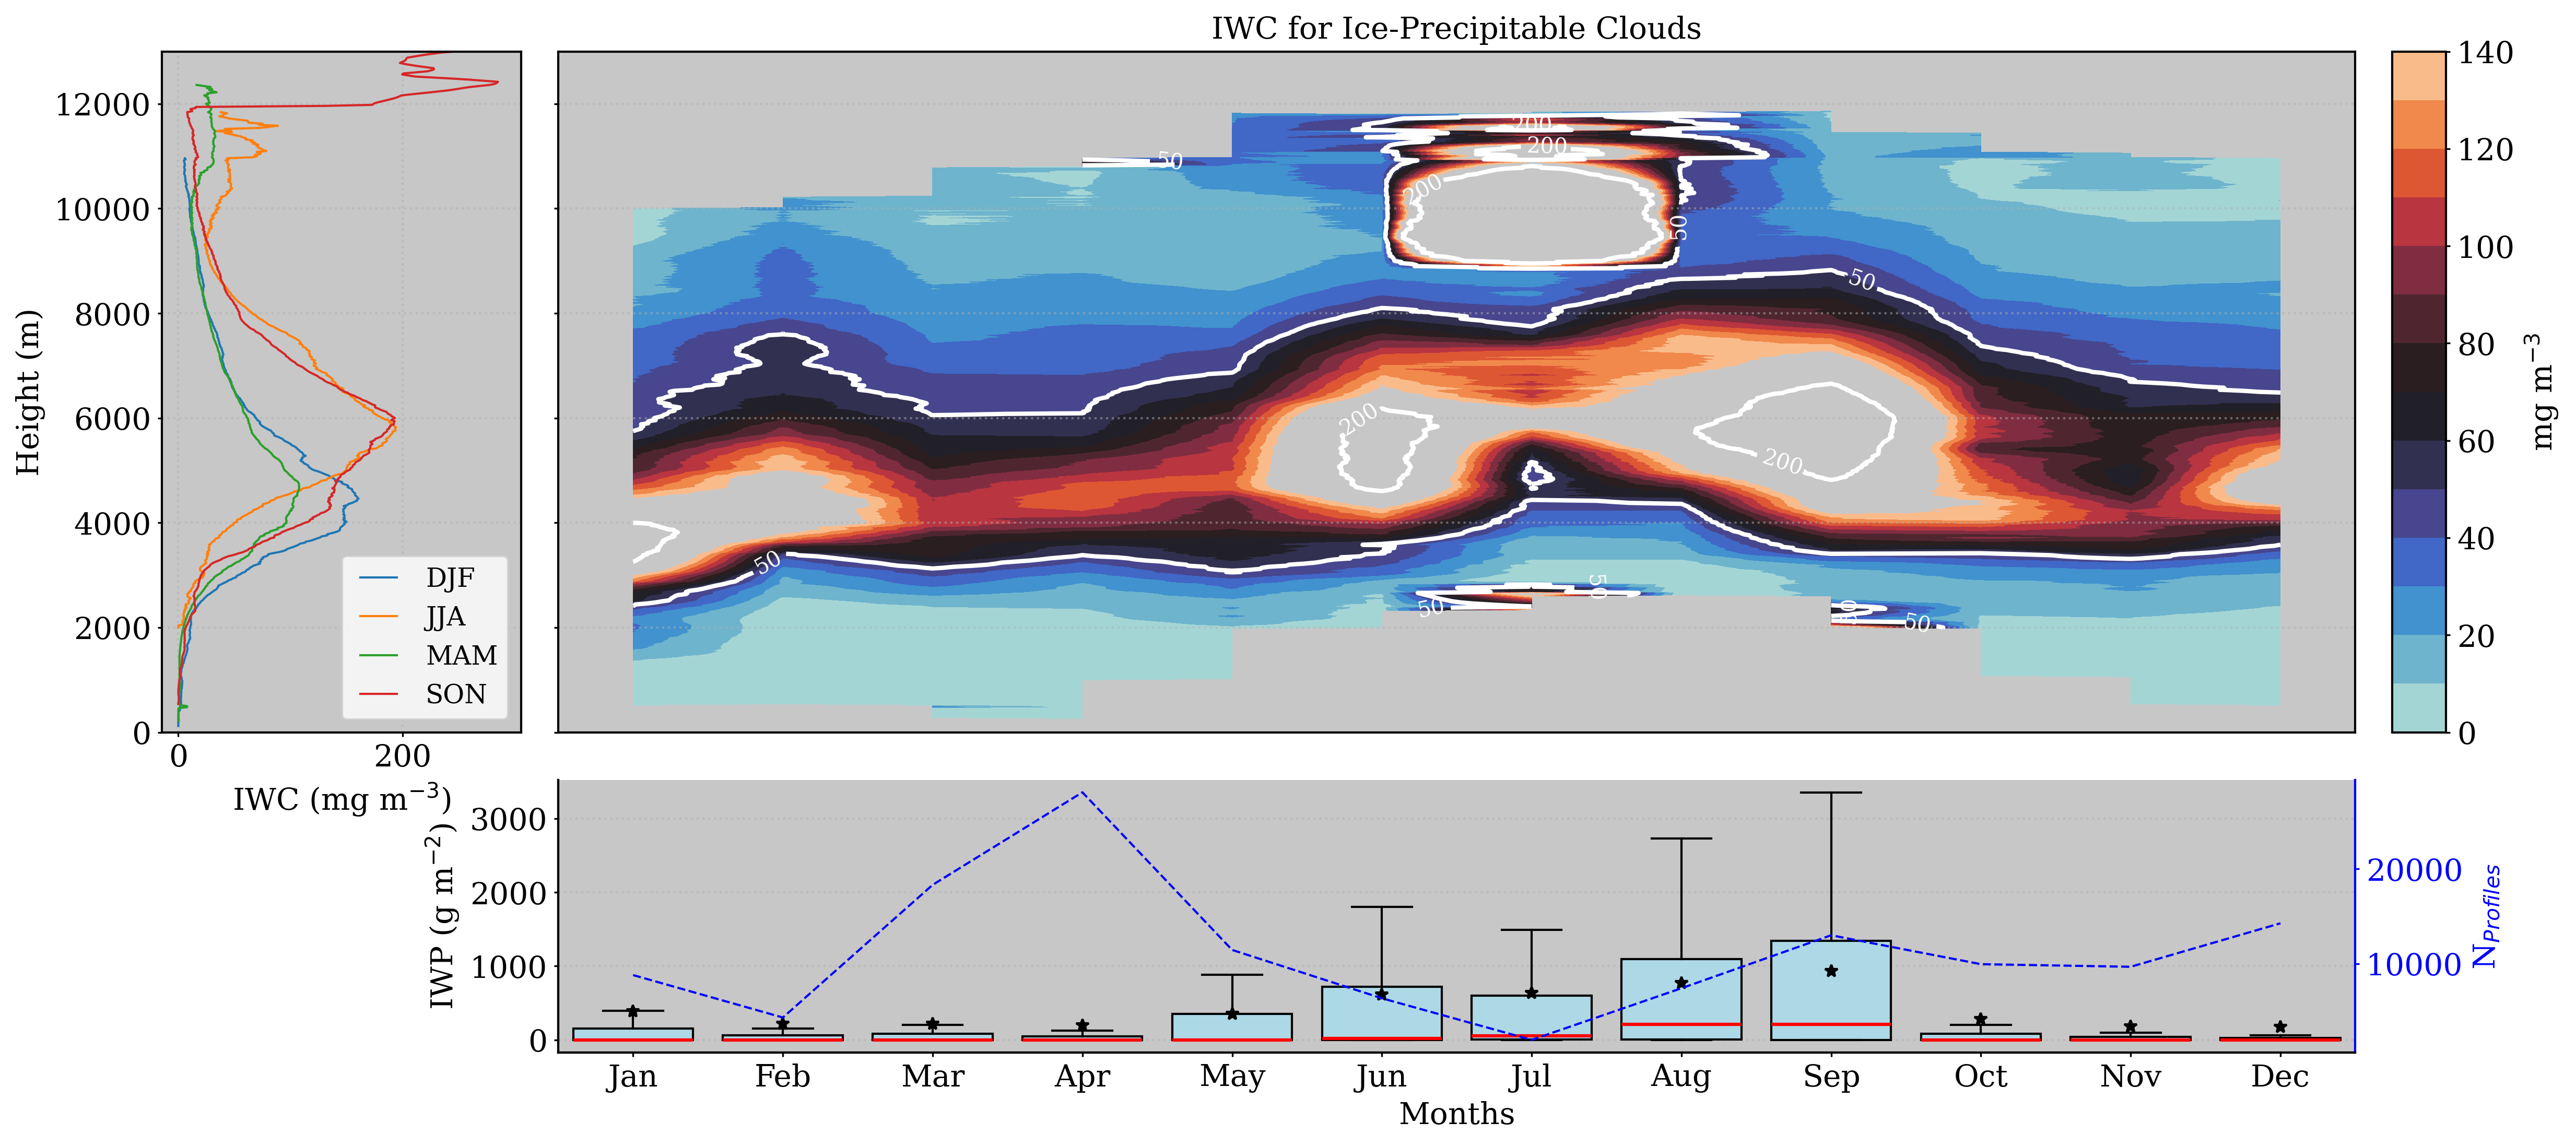
\includegraphics[width=.9\textwidth]{../../phd_clouds/figures/grouped_by_month_evolution_for_iwc_Ice-Precipitable_mesh}
	\caption{Same as Figure \ref{fig:IWC_ice}, but for ice clouds.}
	\label{fig:IWC_ice_prep}
\end{figure}

In relation to the ice effective radius ($r_{ice}$), values below 8 km range from 48 to 64 $\mu$m, with slightly larger particles observed at specific heights during winter and summer—around 5 km in winter and 7 km in summer. Notably, in summer, larger ice particles of 70 $\mu$m can be identified at 10 km, coinciding with higher ice water content (IWC). Such high values can be attributed to strong convective motions, supporting the hypothesis that these summer clouds are cumulonimbus. At the same altitude, $r_{ice}$ values in other months are generally smaller than 30 $\mu$m, except in fall, which also presents higher values at 12 km. The left panel of Figure \ref{fig:IER_ice_prep} depicts a distinct behavior of the median profiles compared to other clouds. Above 1 km, particle size begins to slowly increase (since large particles below are associated with drizzle below the cloud base). For winter and spring, $r_{ice}$ increases up to 5 km (reaching 50 $\mu$m) and then decreases to 20 and 30 $\mu$m, respectively. In contrast, for summer and fall, $r_{ice}$ increases up to 7 km (reaching 50 $\mu$m), then decreases before increasing again to reach second maxima of 50 and 63 $\mu$m, respectively. Despite the larger variability with height, the monthly distribution of $r_{ice}$ shows a highly variable pattern with a sharp mode at the median position of 50 $\mu$m.

\begin{figure}[H]
	\centering
	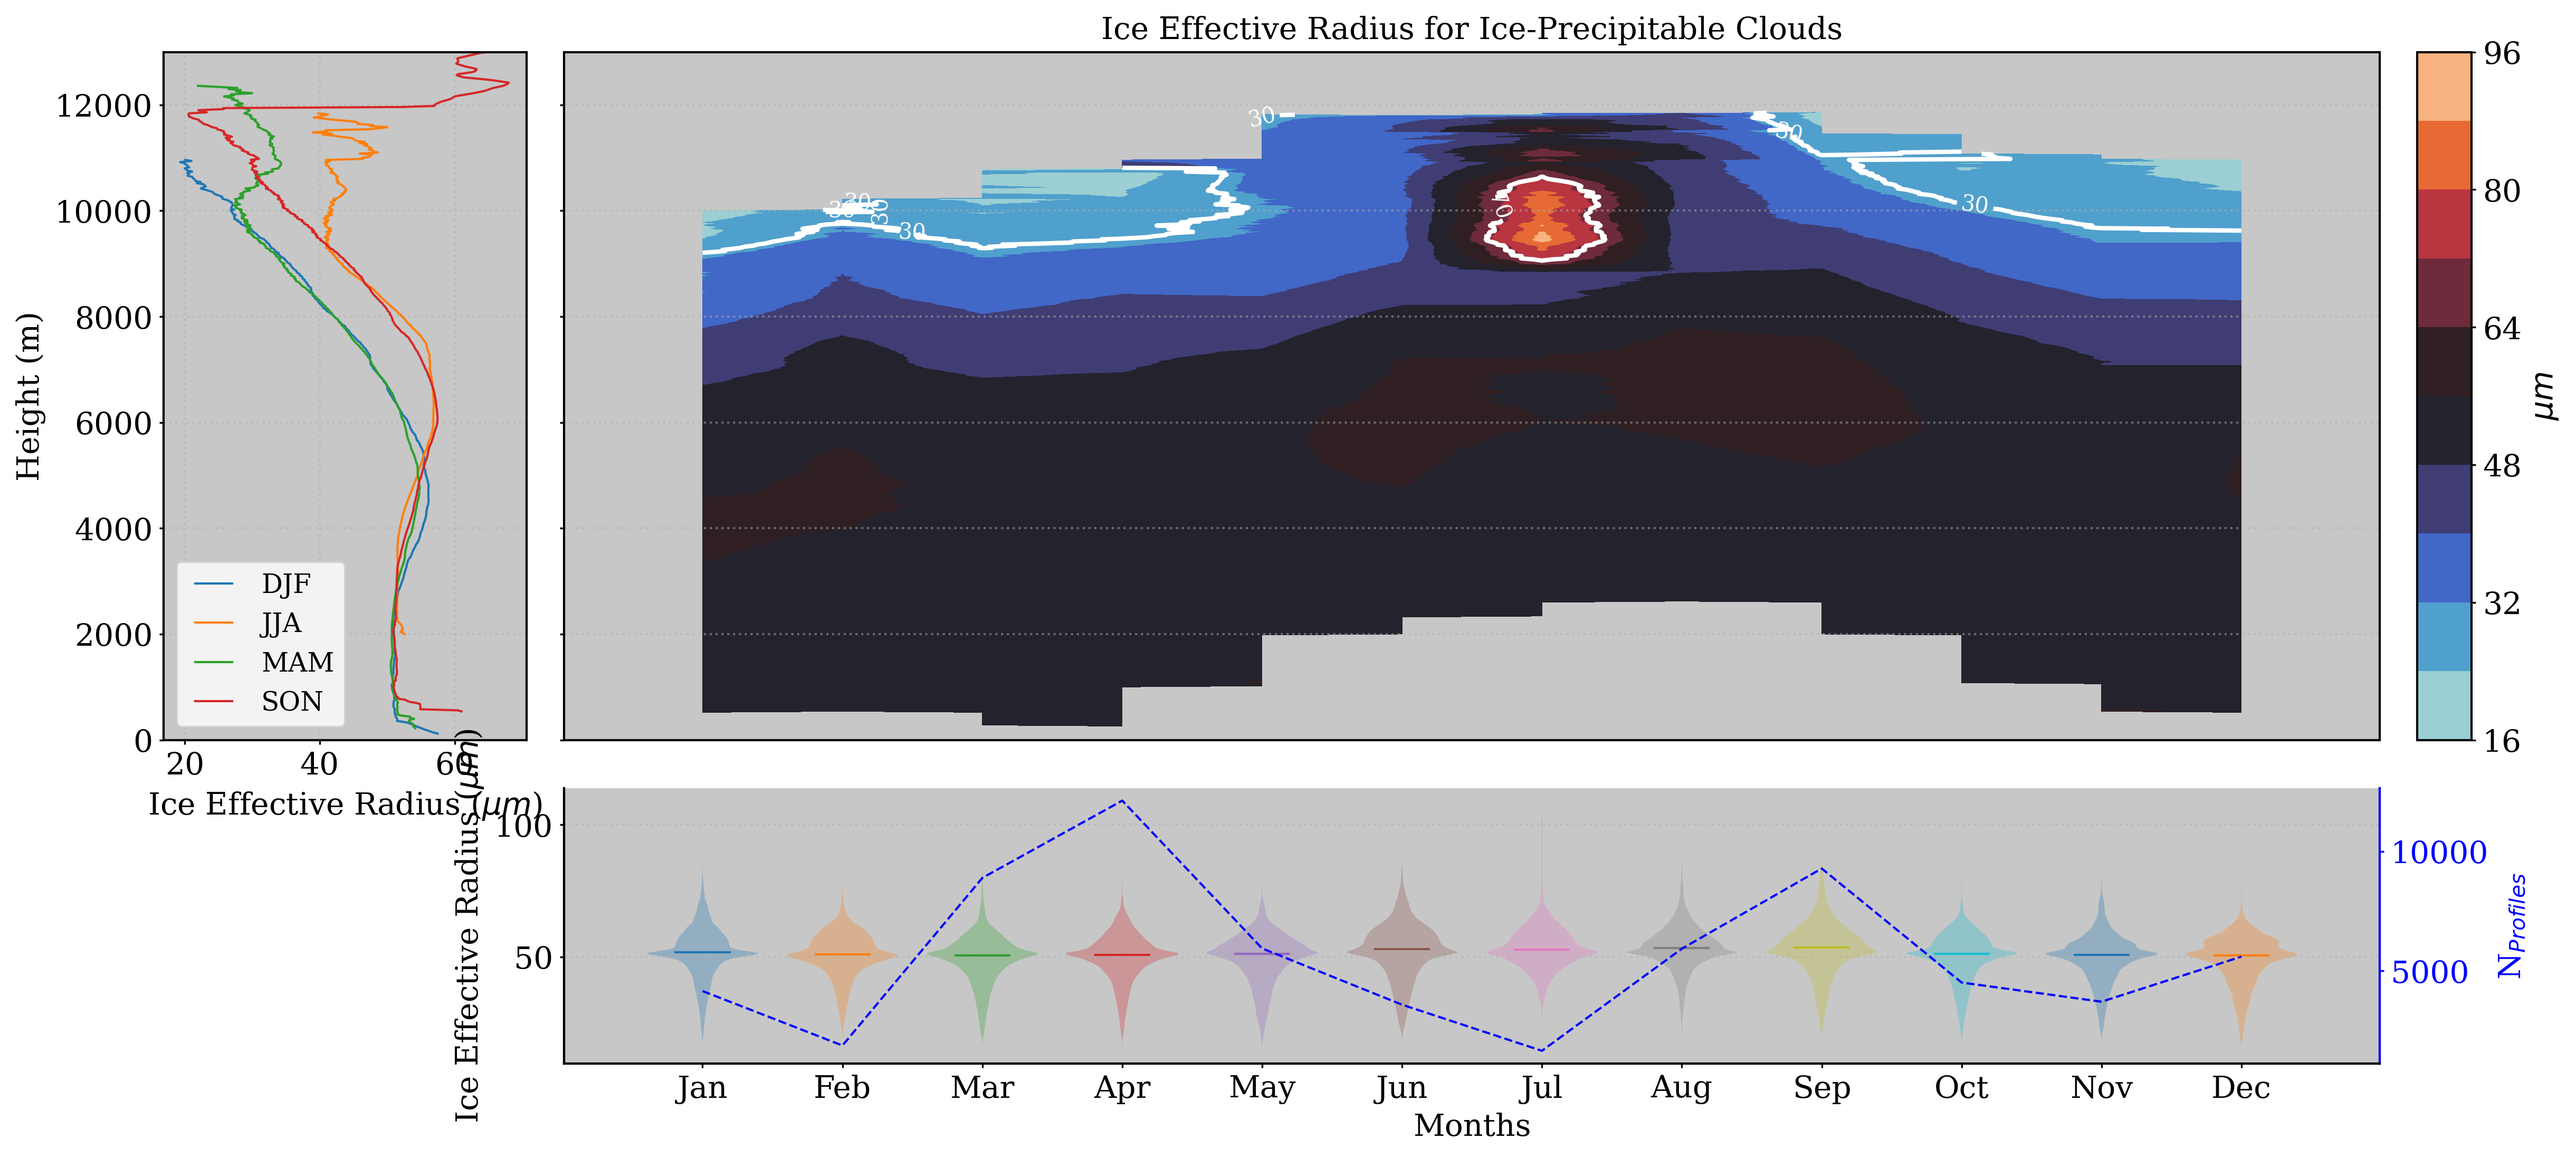
\includegraphics[width=.9\textwidth]{../../phd_clouds/figures/grouped_by_month_evolution_for_ier_Ice-Precipitable_mesh}
	\caption{Same as Figure \ref{fig:IER_ice}, but for mixed-phase clouds.}
	\label{fig:IER_ice_prep}
\end{figure}

In general, these clouds exhibit larger amounts of ice water content (IWC) at mid-levels (4-8 km), particularly in early summer and fall, while other summer months show an ice shortage. In January, most high IWC values were recorded during extreme snowfall events, such as the Filomena and Gloria storms, resulting in high median IWC at low levels during this month. The $r_{ice}$ is also influenced by these snowfalls, showing higher values close to the surface. Typically, $r_{ice}$ ranges around 50 $\mu$m up to 6 km, where it starts to decrease, indicating smaller ice particles in higher-level clouds. Precipitating mixed-phase clouds display a much stronger seasonal pattern in their physical properties. Summer and fall show a peak of IWC at 6 km, while winter and spring exhibit a less pronounced peak at 4 km. These clouds contain significantly more IWC than non-precipitating ice clouds, and they are markedly different, with greater thickness. Similar to precipitating mixed-phase clouds, they have large amounts of IWC and $r_{ice}$ at high levels in summer (> 8 km). Additionally, they demonstrate clear seasonal differences in $r_{ice}$, which is greater in summer and fall
